\chapter{Evaluation procedure and discussion of results}
\label{chap:analysis}

In the previous Chapter, we built a reinforcement learning environment with the use of the components which were described earlier, in Chapter \ref{chap:preliminaries}.
The environment facilitates the simulation of order placement on historical order books of the type described in Chapter \ref{chap:data}.
Furthermore, two agents were introduced: a Q-Learner which learns on private variables; and a Deep Q-Network which learns on market variables.

The aim of this chapter is to make use of this setup and to run simulations, thereby observing whether or not reinforcement learning is indeed capable of optimizing the placement of limit orders.
Therefore, a comprehensive evaluation procedure will be introduced that  measures the capabilities of the reinforcement learning agents.
Throughout this process, real world historical order books will be drawn upon, as well as artificially created order books, whereas the latter define distinctive price trends and eliminate the noise present in real market data.
We first outline the steps of the evaluation procedure.
Subsequently, the real world data sets chosen and their use within the reinforcement learning setup will be described.
Finally, we will evaluate the steps taken in respect of the order that will be used for illustrative purposes.
Accordingly, this chapter will seek to quantify the effectiveness of deep reinforcement learning and its use of the market features previously constructed.

\section{Explanation of the evaluation procedure}
This section explains the evaluation procedure that will be elaborated in the following sections of this chapter. From our analysis of the same, we will aim to formulate a statement that expresses the capabilities of optimizing limit order placement with reinforcement learning and the use of raw market data.
The evaluation steps will proceed chronologically, as follows:
\begin{description}
    \item[Empirical investigation: ]
    Section \ref{sec:eval-empirical} investigates the reinforcement learning environment empirically by simulating an agent's behaviour that places buy and sell orders for a range of limit levels.
    This will provide knowledge about the limitations of the potential optimization possibilities within the given data set and how well we can expect the reinforcement learners to perform.
    \\
    Results: the \textit{estimated returns} to be received for (1) the optimally chosen limit order or (2) an immediate purchase or sale by using a market order.
    
    \item[Q-Learning agent policy: ]
    In Section \ref{sec:eval-qlearn}, we make an attempt to build an order placement policy based on private variables only, by using the Q-Learner.
    This will provide insights into the performance of a naive reinforcement learner and serve as a benchmark for the following simulations proceeded in which we consider market variables.
    \\
    Results: the \textit{average reward} achieved by the Q-Learning agent that uses private variables.

    \item[DQN agent policy: ]
    Section \ref{sec:eval-dqn} applies market variables to the DQN agent.
    Hereby, we make use of Feature I: the price and size of historical orders as described in Chapter \ref{chap:data} (Section \ref{sec:data-feature-1}); as well as Feature II: the price and size of historical trades (described in Section \ref{sec:data-feature-2}).
    As in the previous evaluation step, we will find the average rewards produced by the agent.
    \\
    Results: the \textit{average reward} achieved by the DQN agent with the use of private variables and (1) historical orders or (2) historical trades.

    \item[DQN agent limitations: ]
    Section \ref{sec:eval-dqn-limitations} aims to determine the capabilities and limitations of the DQN agent in greater detail.
    Therefore, we investigate the actions selected by the agent in order to determine the agent's limitations.
    In addition, the agent is applied to an environment which is equipped with an artificially generated order book and will enable us to determine to which extent the agent is able to learn from certain price trends.
    \\
    Results: (1) \textit{insights} into when then DQN agent does not perform well and (2) the \textit{average reward} achieved on order books that follow an artificially created trend (downwards and sine curve).
\end{description}
With the results obtained throughout this evaluation, we will be able to determine and quantify the extent to which deep reinforcement learning can optimize limit order placement; we will also be able to give reasons for its limitations.

\section{Data sets and their usage in the reinforcement learning setup}
\label{sec:analysis-data-sets}
We have selected two $\sim$30 minute samples of historical order book recordings for the experiments in this chapter.
One of the reasons for choosing two very distinguishable data sets is to determine the ability of the learners to react to a variety of market situations.
In addition, as explained in the following section, the expected return of a learner for buying and selling assets heavily depends on the market price movement and therefore the behaviour is expected to be different for the data sets in use.
More precisely, \textit{data set I}, as shown in Figure \ref{fig:sample-down-price}), is a downward trend (indicated by the bid/ask mid-price) and consists of 1132 order book states with a duration of 1681.8 seconds, resulting in 0.67 states per second.
In contrast, \textit{data set II}, as shown in Figure \ref{fig:sample-up-price}, consists of 1469 order book states with a duration of 1746.0 seconds, resulting in 0.84 states per second, which indicates that there was slightly more pressure in terms of orders placed and canceled in this data set.
When reinforcement learning is applied, the data sets are split with ratio $2:1$, resulting in a training set of $\sim$20 minutes and a test set of $\sim$10 minutes.
Although more than two data sets would contribute towards a more generalizes outcome of the evaluation, this was computationally not feasible within this work.
\begin{figure}[H]
    \centering
    \begin{subfigure}[b]{0.45\textwidth}
        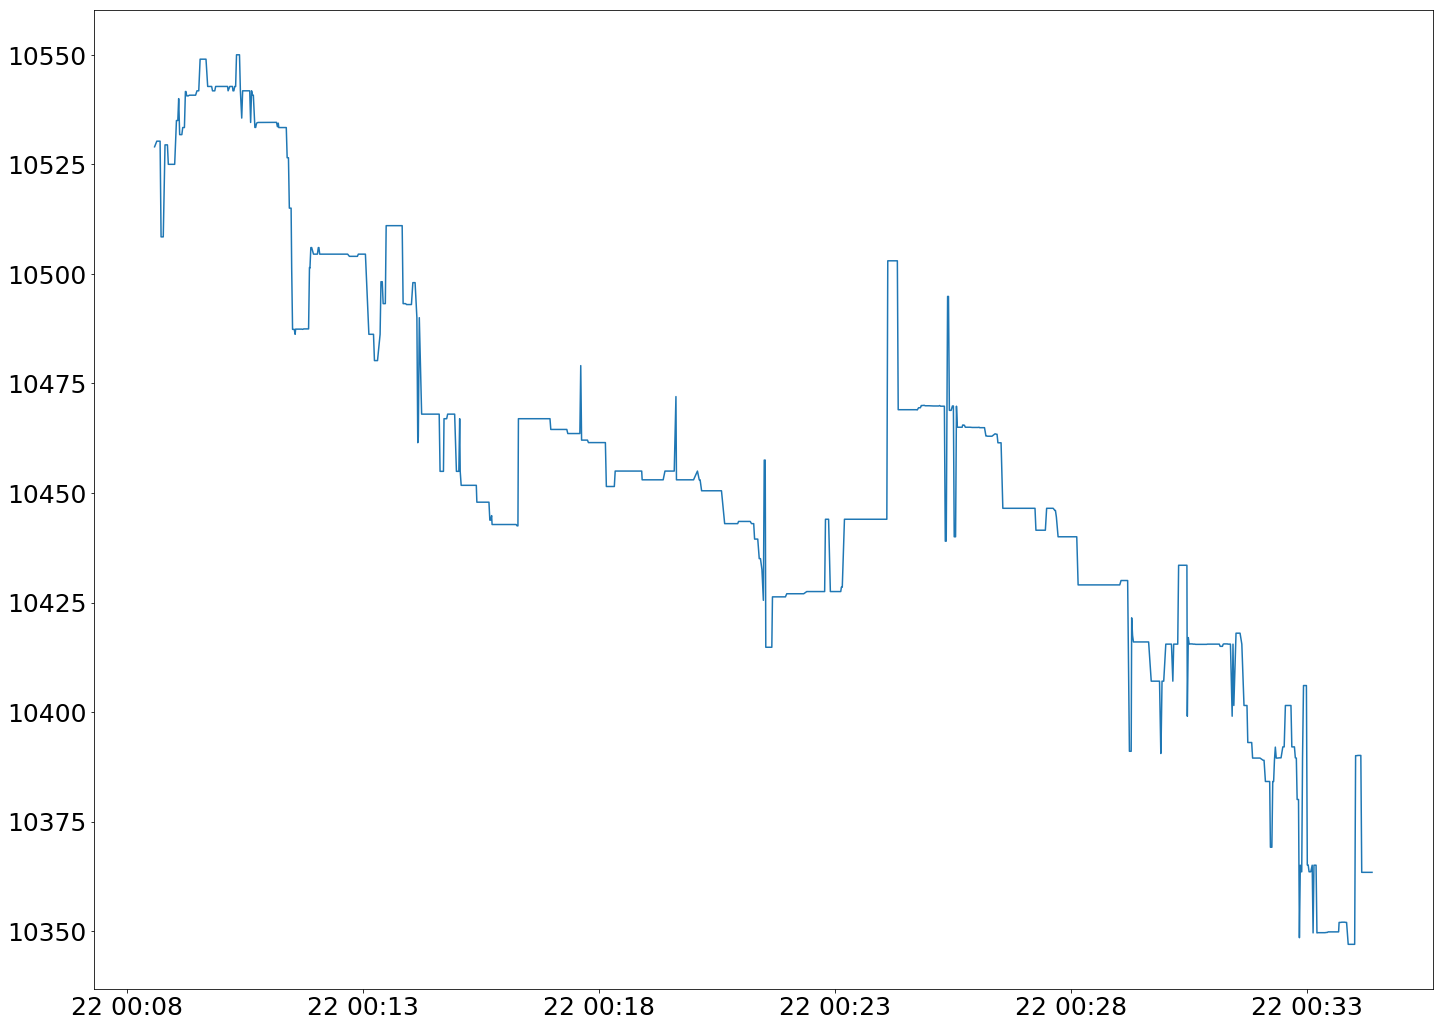
\includegraphics[width=\textwidth]{sample-down-price}
        \caption{30 minute downwards trend}
        \label{fig:sample-down-price}
    \end{subfigure}
    \begin{subfigure}[b]{0.45\textwidth}
        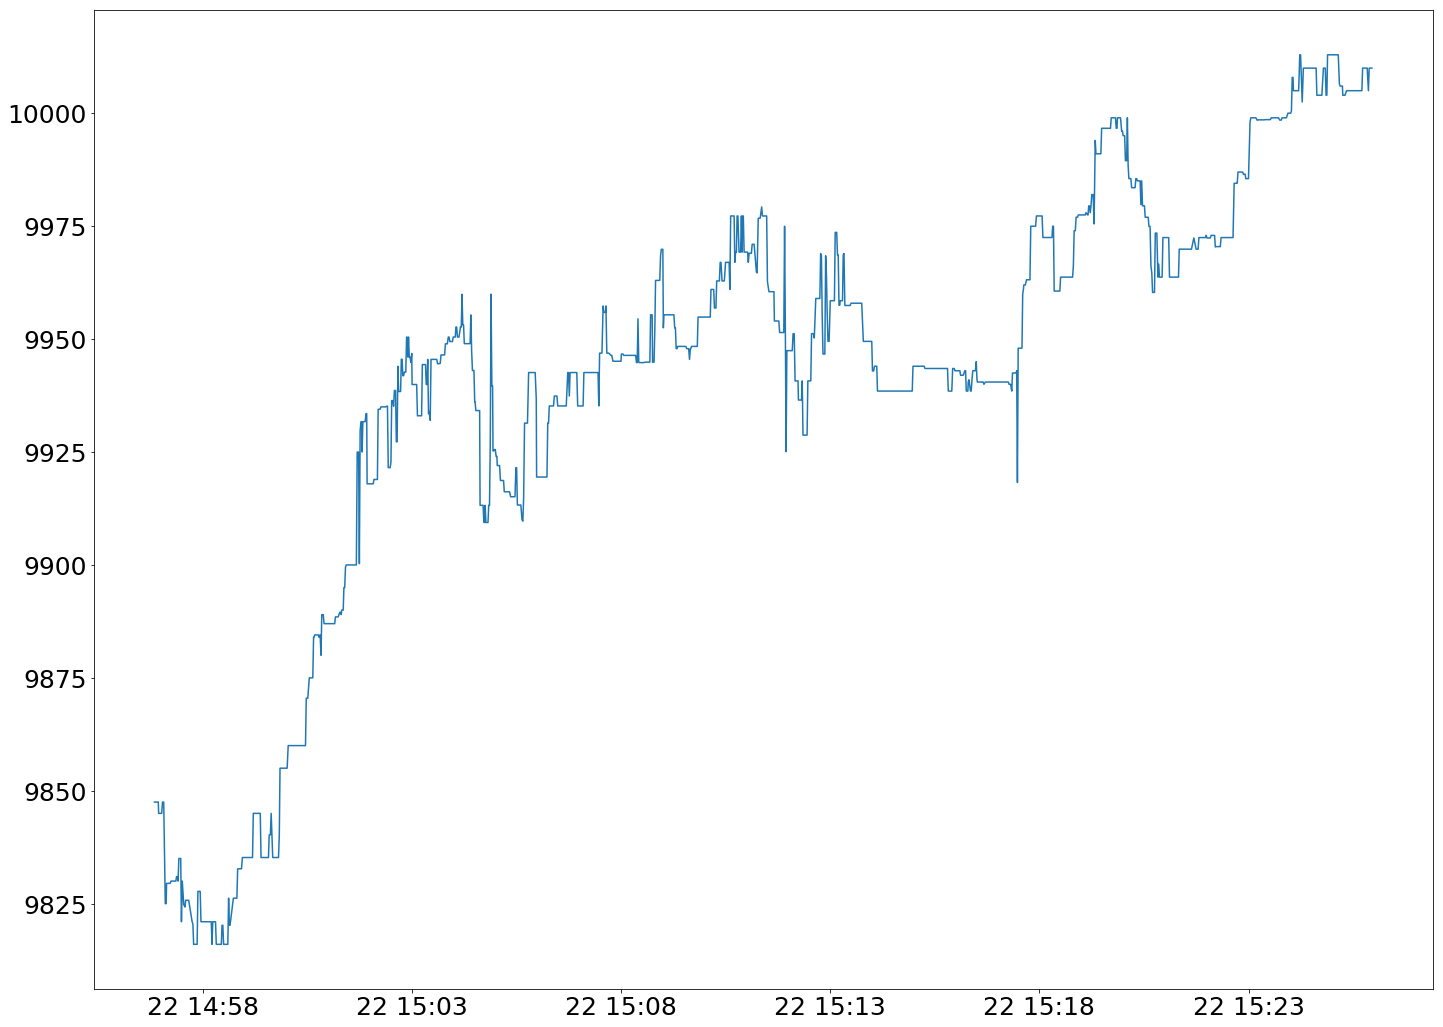
\includegraphics[width=\textwidth]{sample-up-price}
        \caption{30 minute upwards trend}
        \label{fig:sample-up-price}
    \end{subfigure}
    \caption{Bid/ask mid-price of 30 minute order book recordings.}
    \label{fig:sample-price}
\end{figure}

As explained in Chapter \ref{chap:setup}, the historical data sets are not maintained by the reinforcement learning agents directly but instead by the reinforcement learning environment.
The environment provides an observation state $O$, derived from the data set, to an agent, after which the agent decides to take an action $a$ in the form of a limit level.
In turn, the environment prices the order at the received price level and returns the evaluated reward $r$ and the next observation state $O$ to the agent.
In this way, the agent can simulate the placement of limit orders in such a way that, within the given time horizon $H$, the demanded inventory can be either bought or sold.
For each \textit{epoch} an agent deals with, one order, with a specified inventory and time horizon, is defined and is to be filled.
Therefore, the reinforcement learning environment selects, for each epoch the agent initiates, a range of order book states which form the given time horizon $H$ within which the agent is supposed to complete an order.
\begin{figure}[H]
    \centering
    \makebox[\linewidth]{
        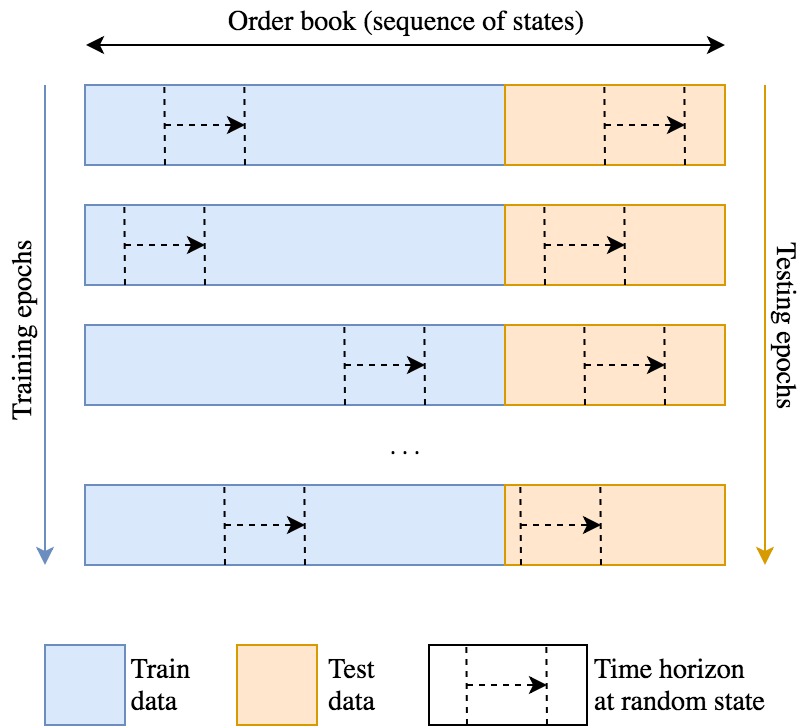
\includegraphics[width=8cm]{images/evaluation-orderbook.png}
    }
    \caption{Order placement training and testing on an order book data set.}
    \label{fig:eval-orderbook-window}
\end{figure}
Figure \ref{fig:eval-orderbook-window} illustrates this process.
A randomly-chosen order book state defines the beginning of the time horizon and the set of order book states that fall into this window.
This is very crucial since the states within this time horizon and the set of states, not only lead to the observation states received by the agent, but also will determine the outcome of the matching process.
More precisely, for each step the agent takes, a consecutive sequence of order book states (with a total difference of their time stamps of $\Delta{t}$) will be considered by the match engine, as explained in the previous chapter in Section \ref{setup:parameters}.
This process is identical for training and testing, except that the underlying data is different and the agent will not learn from the epochs proceeded during testing and instead will report the achieved rewards.

\section{An empirical investigation of the reinforcement learning environment}
\label{sec:eval-empirical}
In this section, the relationship between the limit order placement and the received return will be investigated.
The methods demonstrated are based on the related work described in Section \ref{sec:related-execution-behaviour} and provide the ability to empirically evaluate the reinforcement learning environment (Chapter \ref{chap:setup}).
Therefore, we simulate an agent that submits actions in order to buy and sell shares at every possible limit level and records the immediate returns it receives.
A return is defined as the difference between the market price prior to the order placement and the volume- weighted average price (VWAP) paid or received, as stated in Eq. \ref{setup:reward}.
As a result, we gain an understanding of the estimated rewards of limit order placement using the given historical data set.
In addition, these results set a benchmark for the reinforcement learners to come.

We will now describe the setup of this investigation.
We investigate the rewards of limit orders placed on progressively increasing time horizons, from 10 seconds to 100 seconds, and thereby observe the importance of the action chosen by the agents in order to buy or sell assets, in accordance with the length of the time horizon.
For each time horizon, we place (e.g. cross-validating) 100 orders of size 1.0 BTC at the beginning of the time horizon whose beginning is defined by a randomly-chosen order book state. 
A market order follows for the remainder of shares (if any) once the time horizon is consumed.
The expected return is then derived from the average of the received returns of these 100 orders.
This process is repeated across a range of 201 actions $A$ that correspond to the limit levels $-100...100$ with step size $\Delta{a} = \$0.10$, resulting in orders priced in the range of $p_m-10 \ \dots \ p_m+10$, whereas $p_m$ is the market price before the order was placed.
The limit levels are chosen broadly in order to retrieve understanding about the outcome of a variety of possible actions.
Hence, a total of 20,100 orders are submitted for each time horizon defined.
Finally, the investigation is undertaken for both data sets I and II.

\subsection{Order placement behavior on data set I}
For data set I, where the market sees a downwards trend, the intuition is as follows:
We expect buy orders to result in better returns when placed deep in the order book, in other words, on orders that have a highly negative limit level ($a<0$).
Since the price tends to fall, the assumption is that an agent is able to buy at a lower price once time has passed.
Therefore, the longer the time horizon, the lower the limit level that can still be chosen in order to execute the full amount of shares.
In contrast,  we expect sell orders to provide better returns when the agent crosses the spread with a positive limit level ($a>0$).
The assumption is that, in a falling market, it is unlikely that market participants are willing to buy at higher prices and therefore the agent must place sell orders higher in the book in order to sell immediately.
Otherwise, the longer the time horizon, the less return an agent would retrieve as the market order, that is submitted if the order has not been filled, becomes costly.
This investigation is shown in Figure \ref{fig:behvaiour-down} for time horizons of 10, 30, 60 and 100 seconds.
The x-axis indicates the placement of the order at limit levels ranging from $a=-100$ to $a=+100$ and the y-axis indicates the average return received.

With a time horizon of only 10 seconds left, the expected behavior is, however, proven wrong.
For buy orders, shown in Figure \ref{fig:behvaiour-down-10s-buy}, the returns suggest that orders be placed close to the spread, but still on the opposing side, at a limit level of $\sim$+5.
The spike at limit level $\sim$-5 indicates that the overall best return was produced at this level. However, this comes with the risk that the orders fail to execute, which is indicated by the downward spike also close to level $\sim$-5.
For selling within 10 seconds, as shown in Figure \ref{fig:behvaiour-up-10s-sell}, the best return is given when crossing the spread with a positive limit level of $\sim$+50.

With an increased time horizon of a total of 30 seconds, as shown in Figures \ref{fig:behvaiour-down-30s-buy} and \ref{fig:behvaiour-down-30s-sell}, the expected behavior becomes more apparent.
Positive returns can be achieved by posting buy orders deep in the order book.
Therefore, we can expect that in the given market situation, an agent would be able to partially execute the order at very low limit levels and, for the unexecuted part, a market order would follow.
The densest range of positive returns can be seen around the limit levels just below the spread.
Orders placed deeper in the book oftentimes result in slightly lower returns, which indicates that the orders were only filled partially and expensive market orders followed.
Crossing the spread causes increasingly lower returns, the more positive the limit level is chosen, as a result of agents' willingness to immediately buy at an increasing price.
The opposite effect occurs while selling assets.
Market orders higher in the book result in better returns than limit orders deep in the book.
Interestingly, orders which were placed very deep in the book, at limit level $\sim$-50 and below, are rewarded better than the ones close to the spread.
The most likely reasons it that a minority of orders  were partially filled at this level during the cross-validation process.

With time horizons of 60 and 100 seconds, the expected behavior of the orders is clearly apparent.
Buy orders, as shown in Figures \ref{fig:behvaiour-down-60s-buy} and \ref{fig:behvaiour-down-100s-buy}, achieve highest returns when placed very deep in the order book.
However, when placed too deep, at levels -100, the returns are slightly lower as a result of unexecuted orders which had to be completed with market orders.
In addition, positive limit levels become stable at this range since there are more sellers in the market with the extended time horizon.  Therefore, very highly placed orders have the same effect as limit orders posted only slightly above the spread.
Furthermore, placing orders very deep in the book has the same effect as when placing them just below the spread; that is, there are no traders willing to buy at such a high price and therefore market orders follow once time has passed.
\vfill
\newpage
\begin{figure}[H]
    \centering
    \begin{subfigure}[b]{0.45\textwidth}
        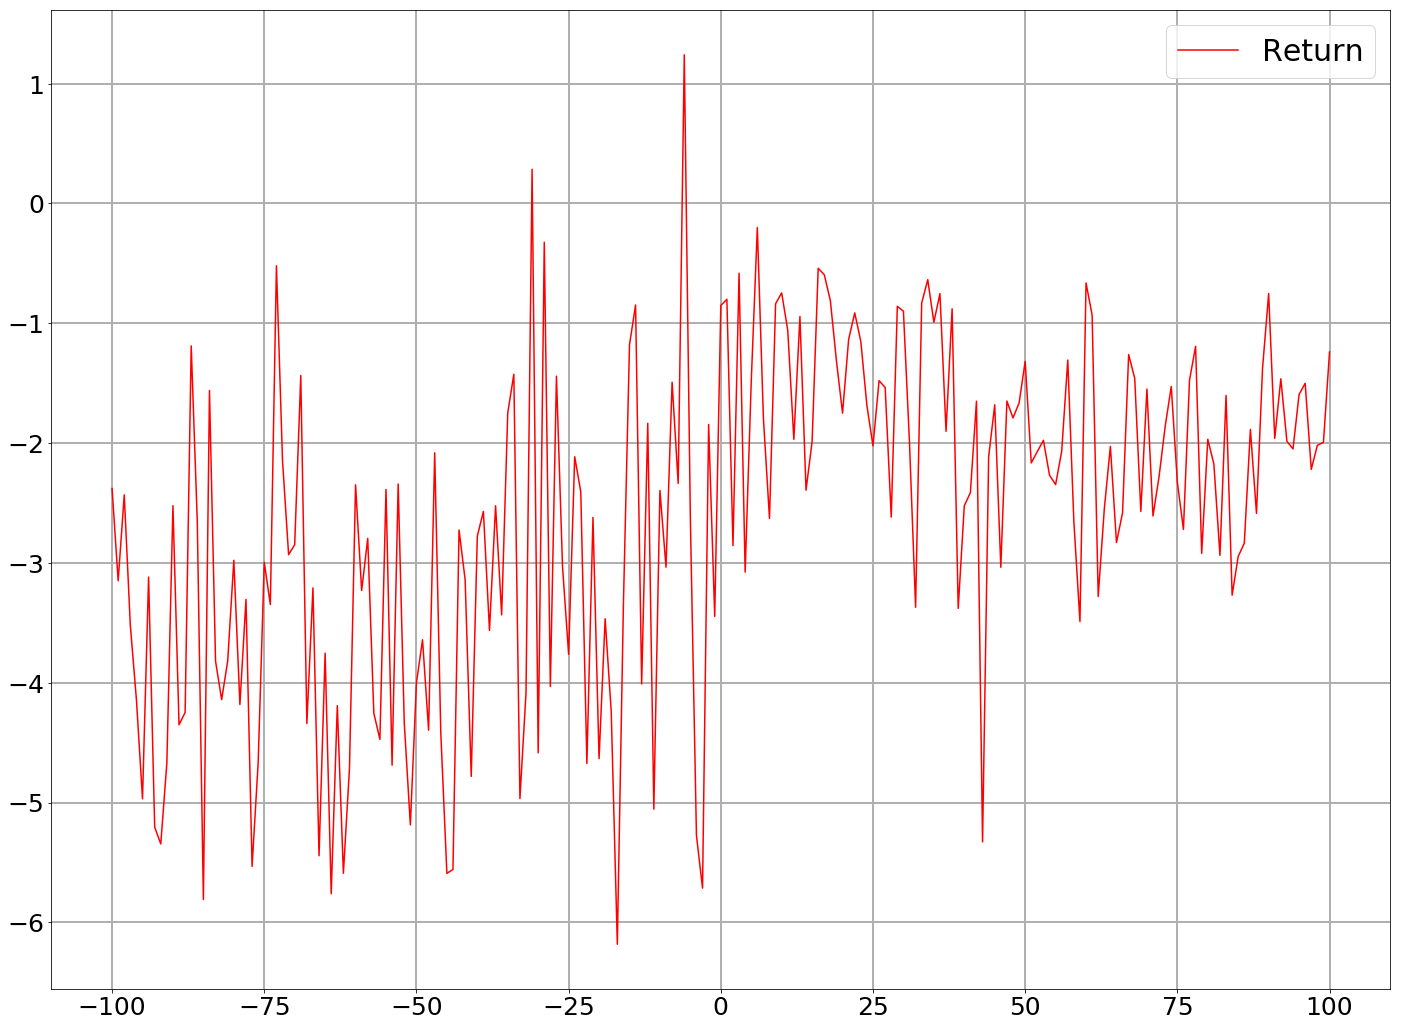
\includegraphics[width=\textwidth]{images/behaviour-10s-buy.png}
        \caption{Returns of buy orders within 10 seconds}
        \label{fig:behvaiour-down-10s-buy}
    \end{subfigure}
    \begin{subfigure}[b]{0.45\textwidth}
        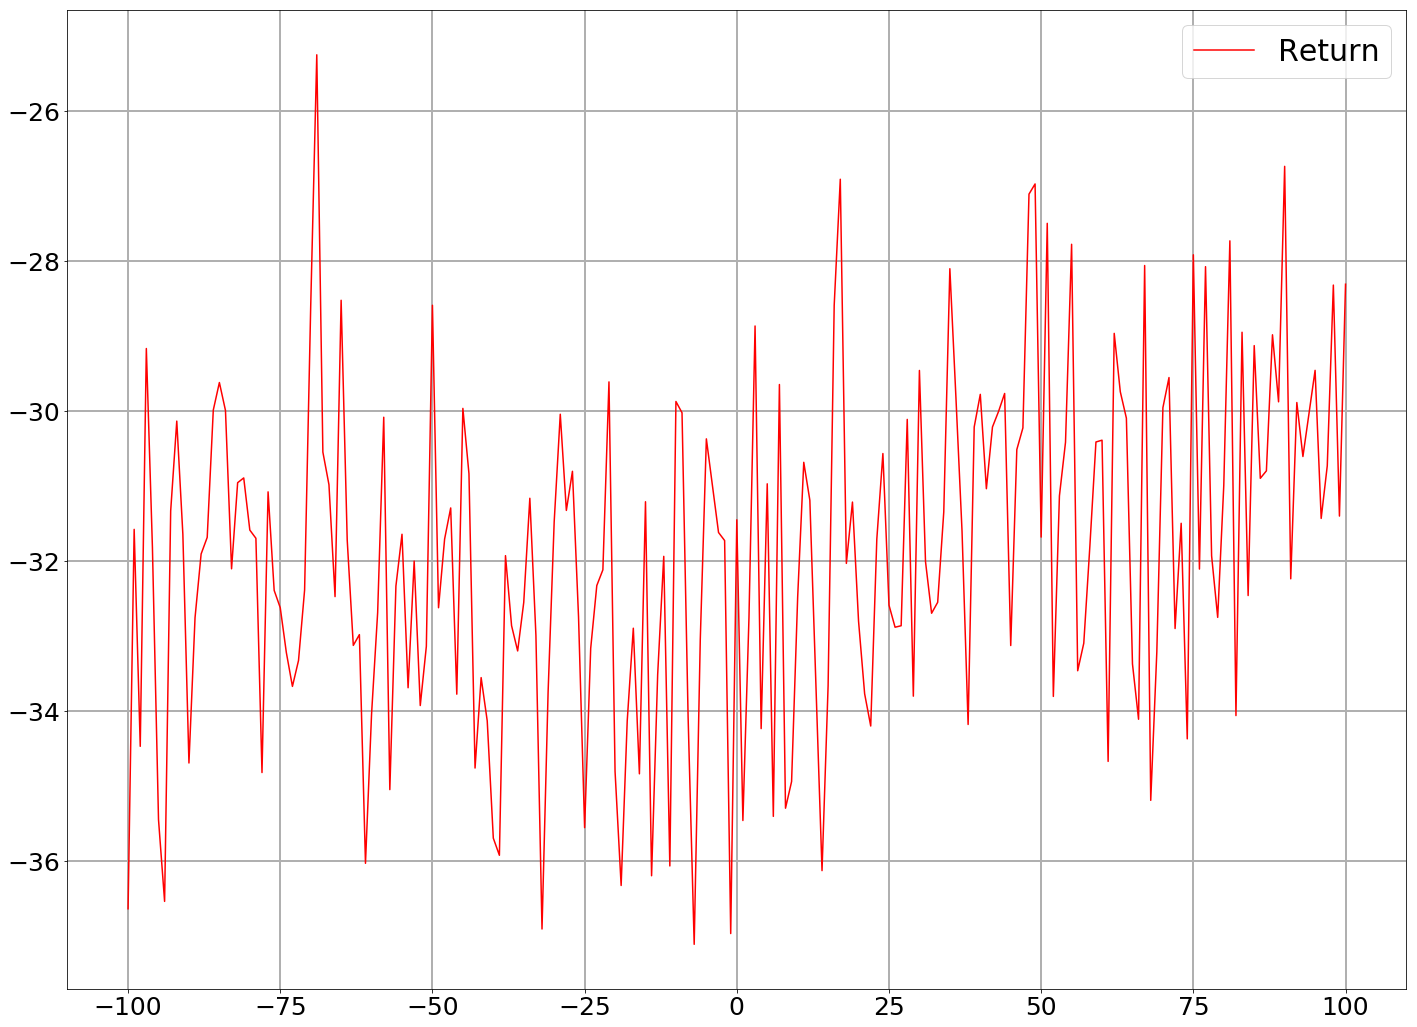
\includegraphics[width=\textwidth]{images/behaviour-10s-sell.png}
        \caption{Returns of sell orders within 10 seconds}
        \label{fig:behvaiour-down-10s-sell}
    \end{subfigure}
    \begin{subfigure}[b]{0.45\textwidth}
        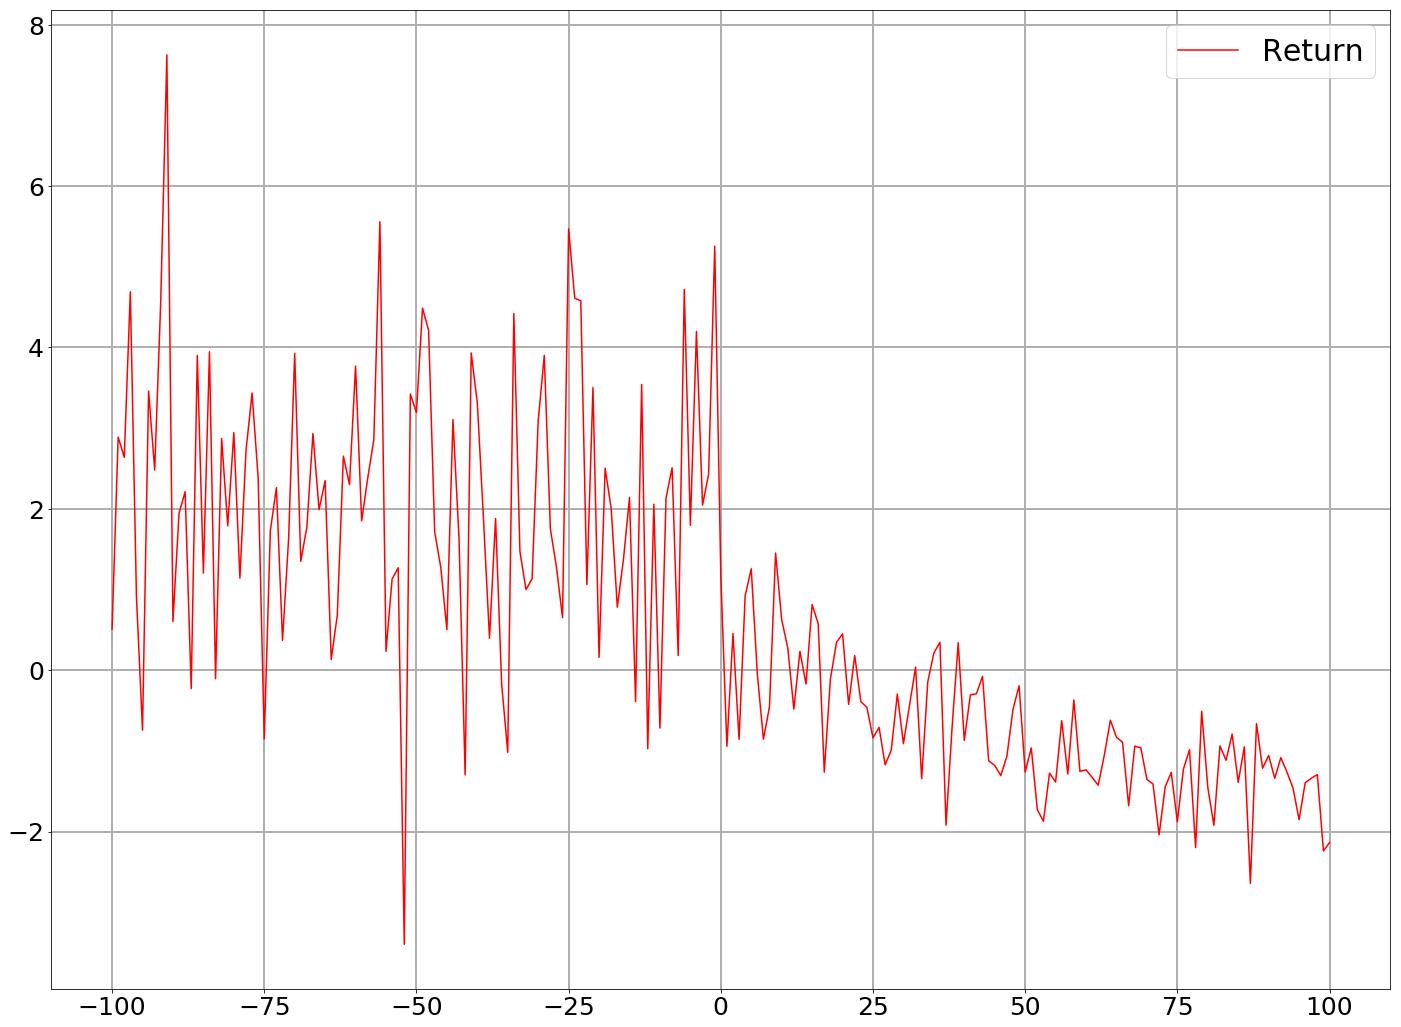
\includegraphics[width=\textwidth]{images/behaviour-30s-buy.png}
        \caption{Returns of buy orders within 30 seconds}
        \label{fig:behvaiour-down-30s-buy}
    \end{subfigure}
    \begin{subfigure}[b]{0.45\textwidth}
        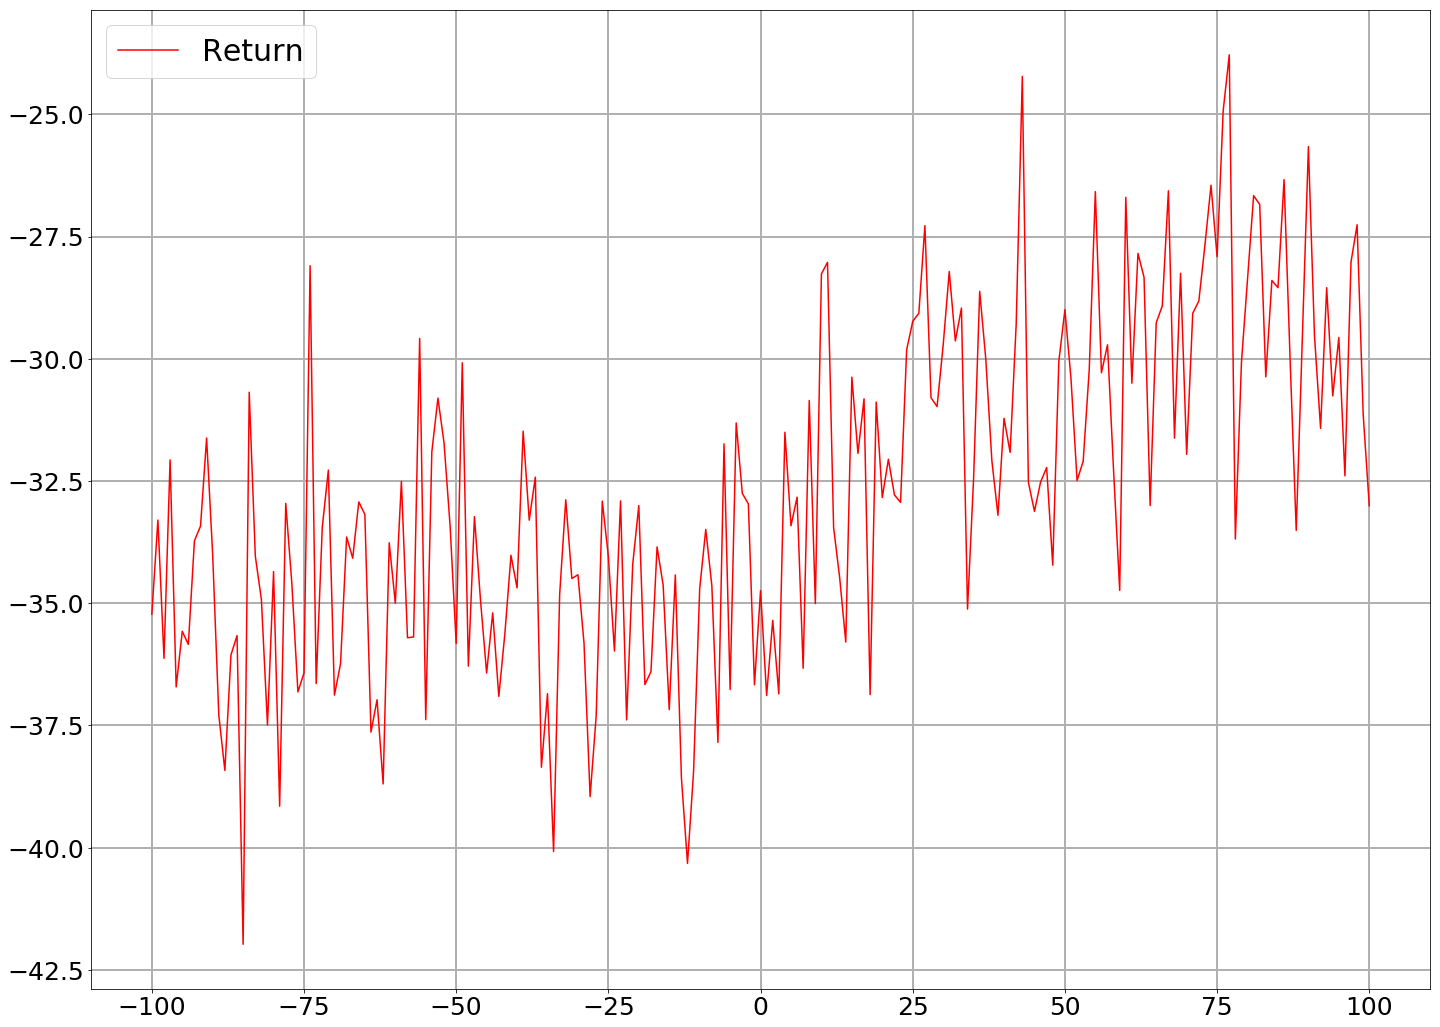
\includegraphics[width=\textwidth]{images/behaviour-30s-sell.png}
        \caption{Returns of sell orders within 30 seconds}
        \label{fig:behvaiour-down-30s-sell}
    \end{subfigure}
    \begin{subfigure}[b]{0.45\textwidth}
        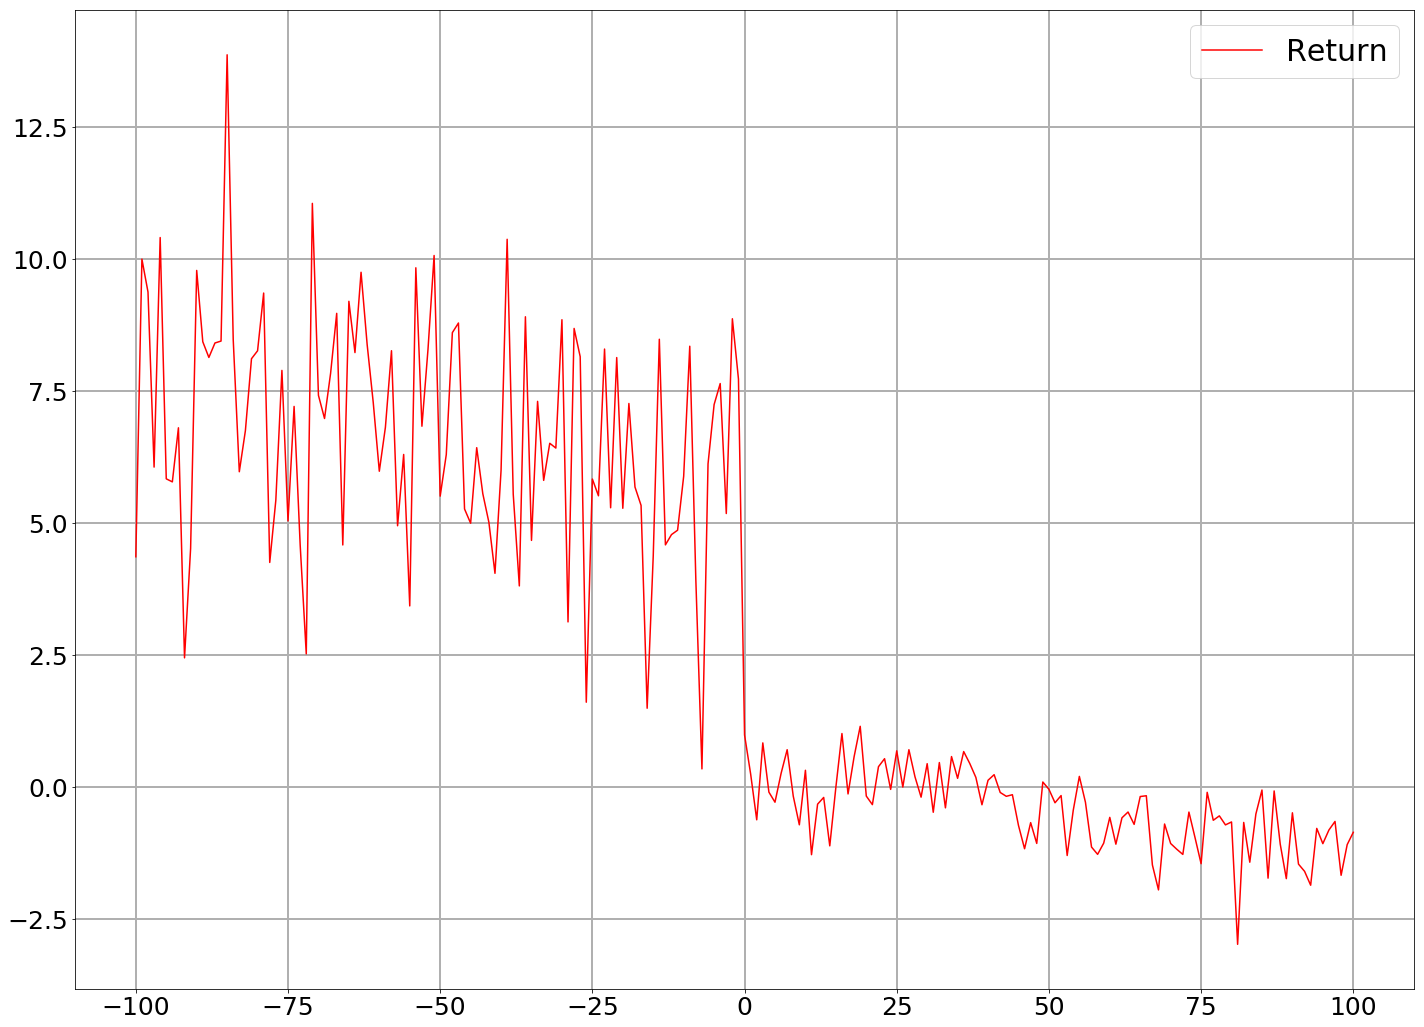
\includegraphics[width=\textwidth]{images/behaviour-60s-buy.png}
        \caption{Returns of buy orders within 60 seconds}
        \label{fig:behvaiour-down-60s-buy}
    \end{subfigure}
    \begin{subfigure}[b]{0.45\textwidth}
        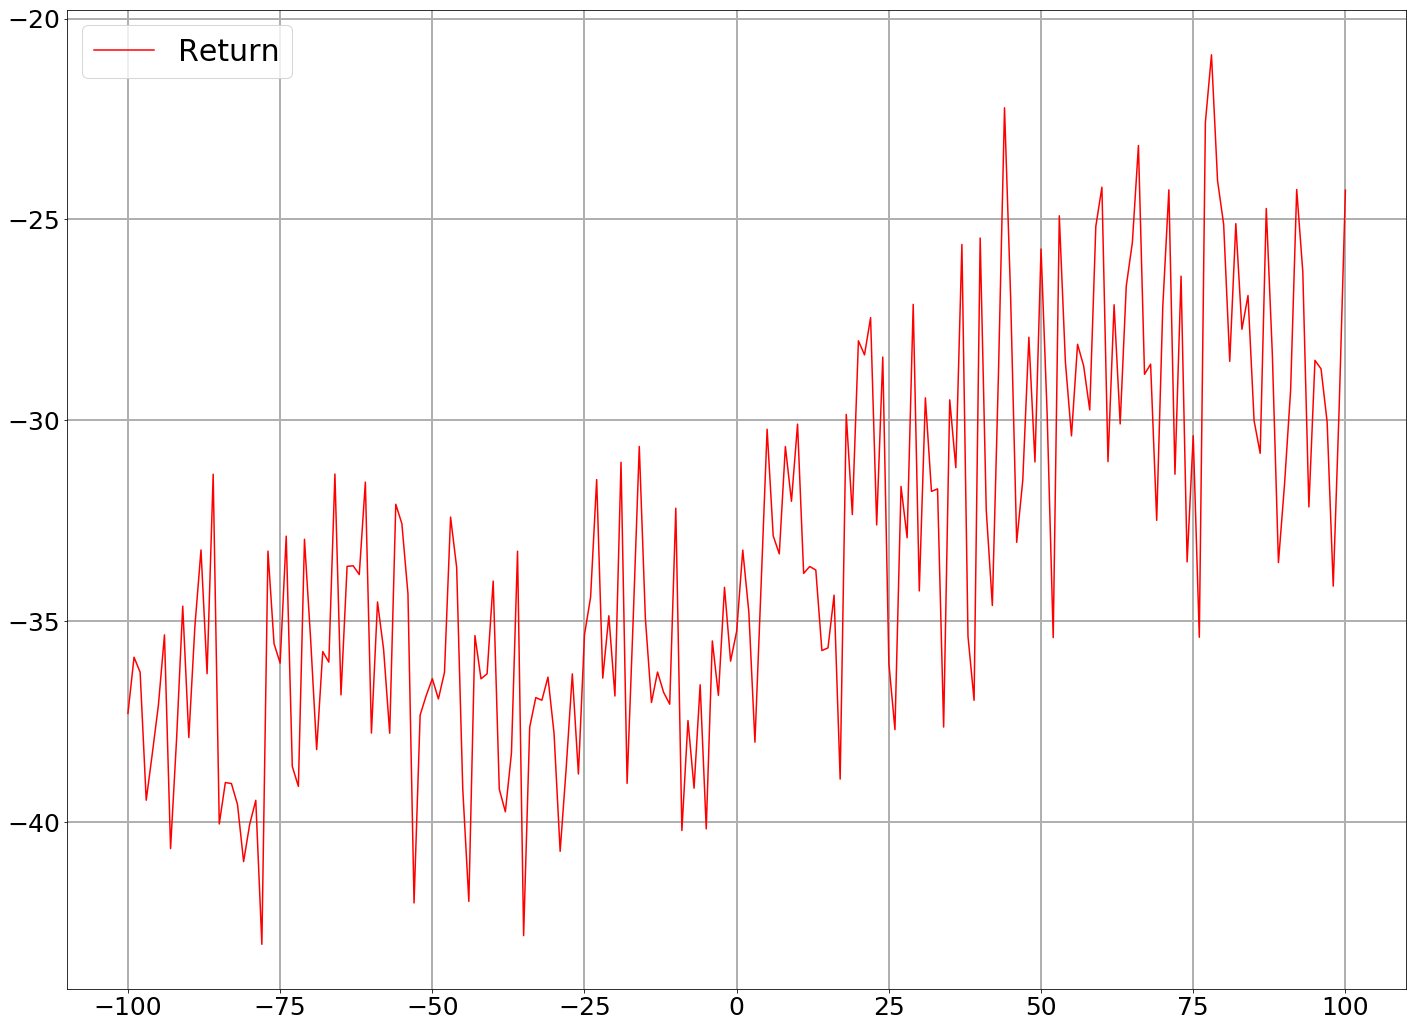
\includegraphics[width=\textwidth]{images/behaviour-60s-sell.png}
        \caption{Returns of sell orders 60 seconds}
        \label{fig:behvaiour-down-60s-sell}
    \end{subfigure}
    \begin{subfigure}[b]{0.45\textwidth}
        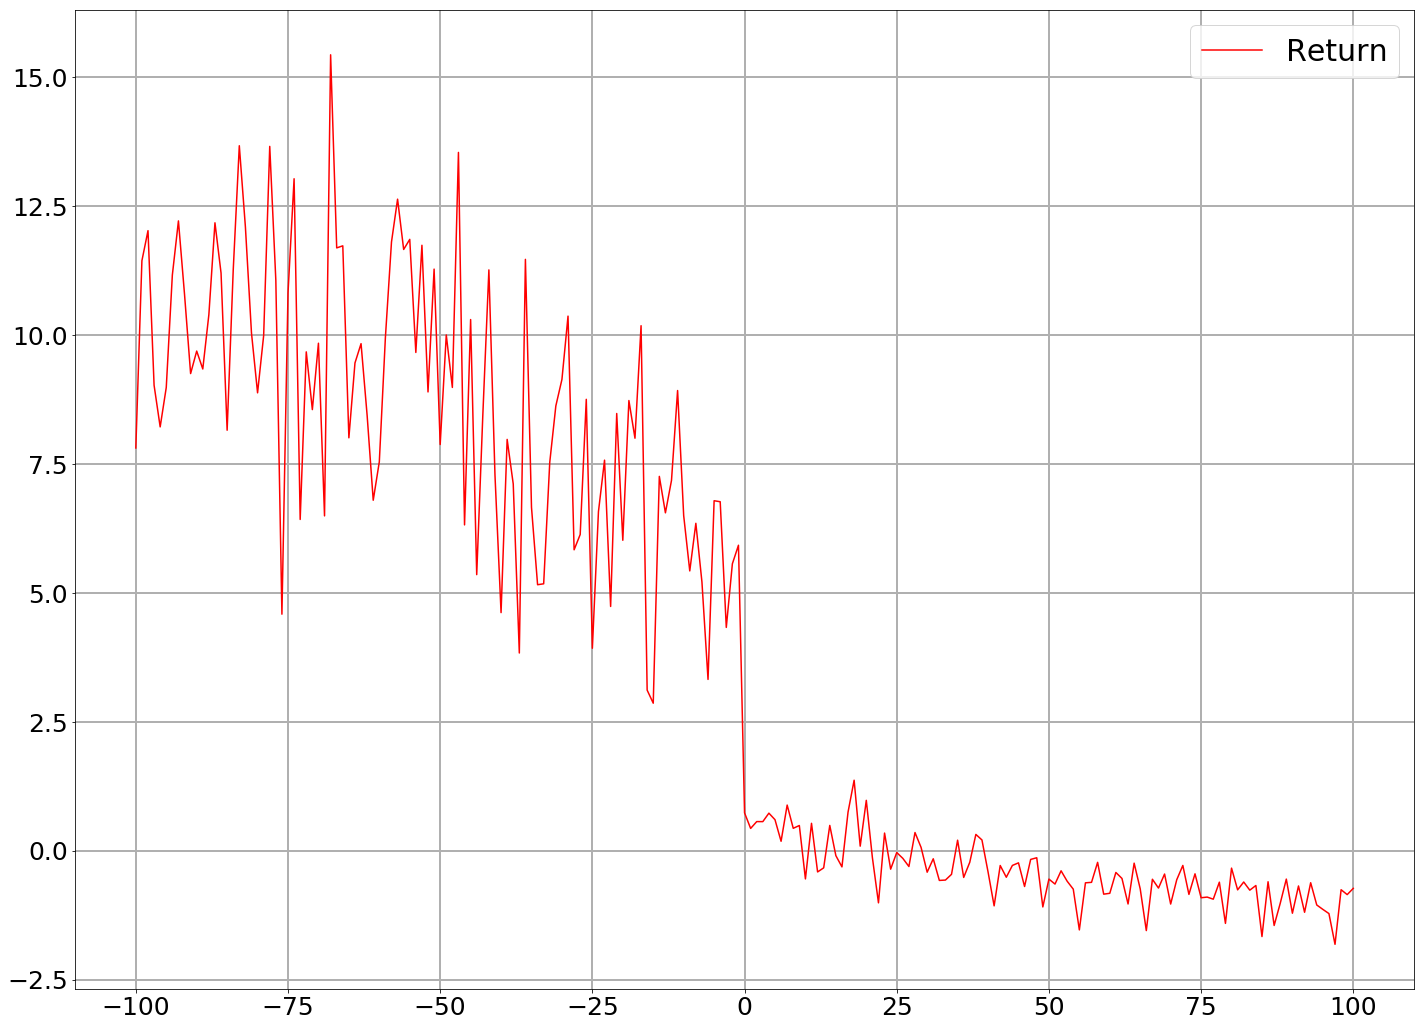
\includegraphics[width=\textwidth]{images/behaviour-100s-buy.png}
        \caption{Returns of buy orders 100 seconds}
        \label{fig:behvaiour-down-100s-buy}
    \end{subfigure}
    \begin{subfigure}[b]{0.45\textwidth}
        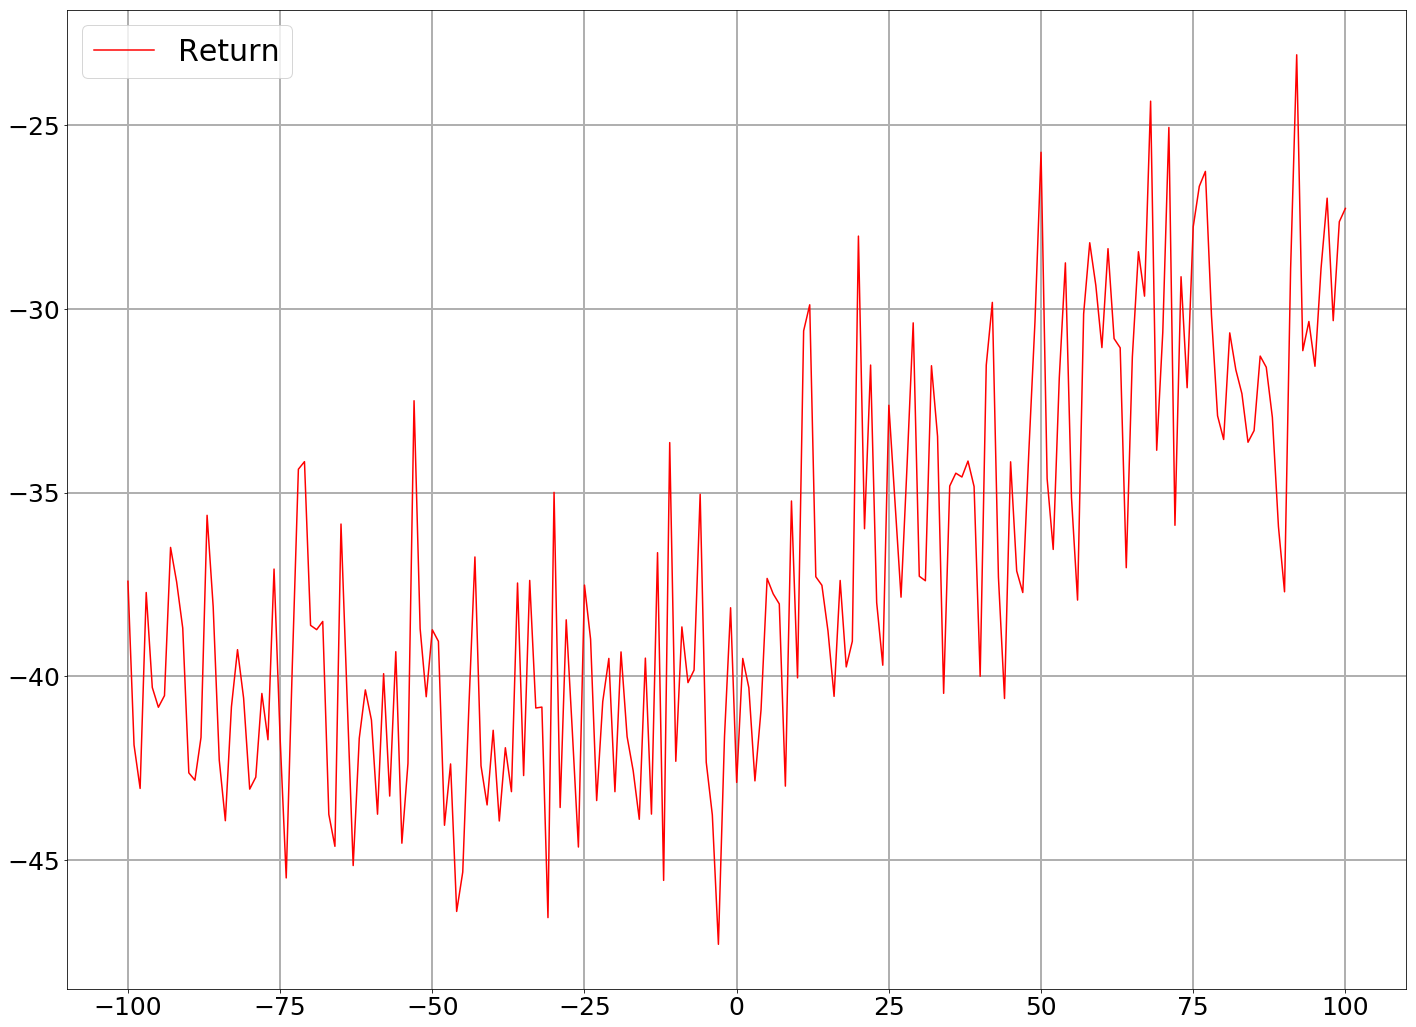
\includegraphics[width=\textwidth]{images/behaviour-100s-sell.png}
        \caption{Returns of sell orders 100 seconds}
        \label{fig:behvaiour-down-100s-sell}
    \end{subfigure}
    \caption{Returns of buy and sell orders executed within 10, 30, 60 and 100 seconds on data set I.}
    \label{fig:behvaiour-down}
\end{figure}

\begin{figure}[H]
    \centering
    \begin{subfigure}[b]{0.45\textwidth}
        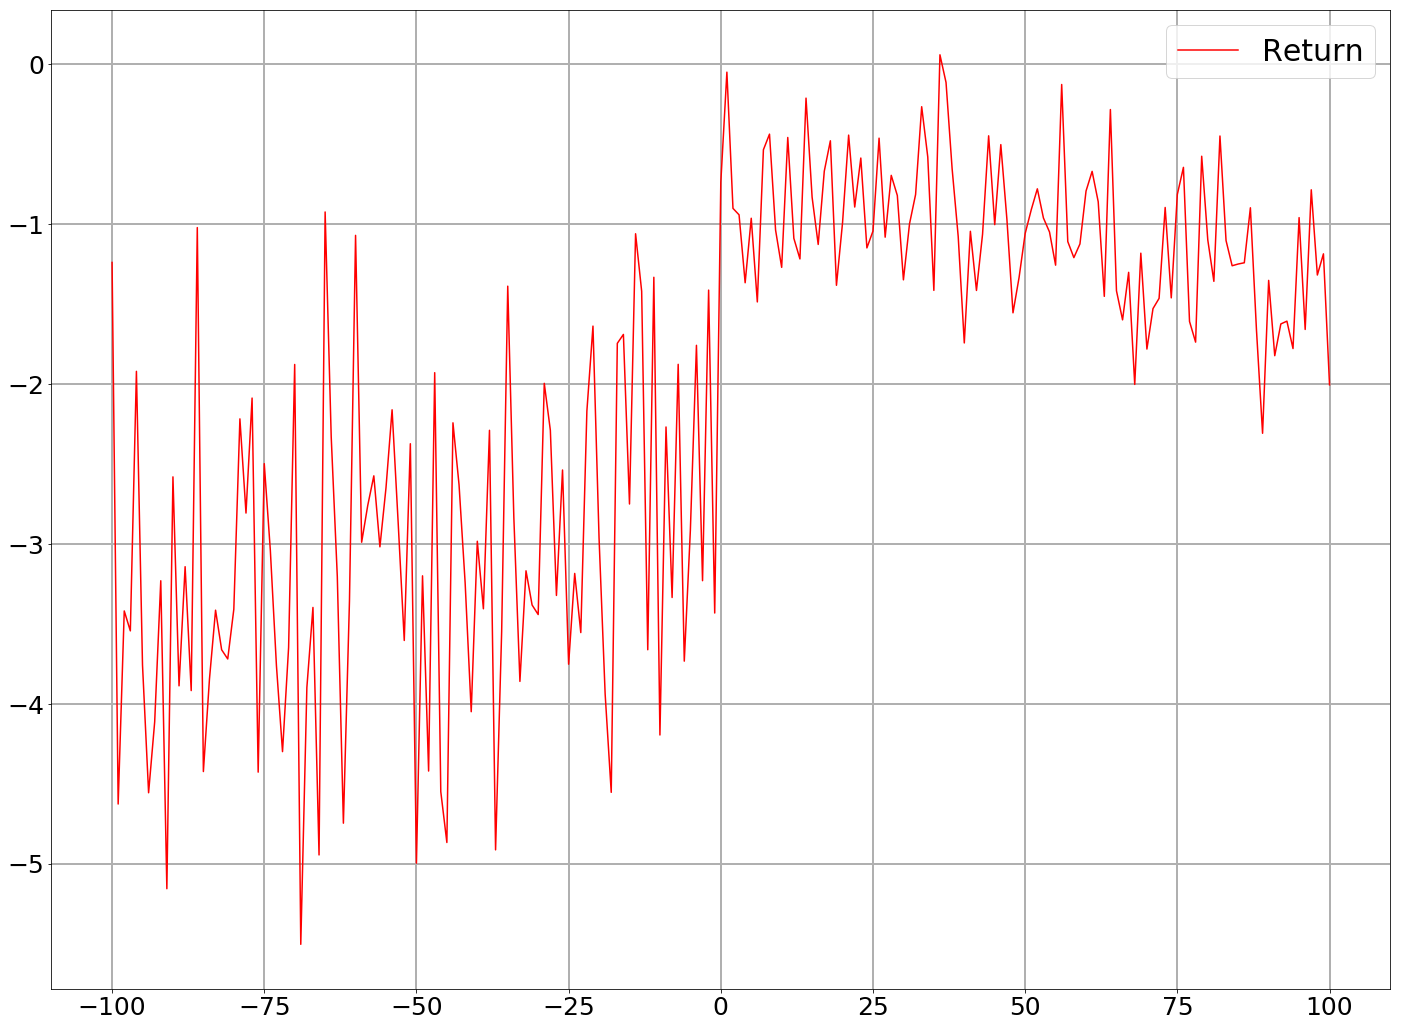
\includegraphics[width=\textwidth]{images/behaviour-up-10s-buy.png}
        \caption{Returns of buy orders within 10 seconds}
        \label{fig:behvaiour-up-10s-buy}
    \end{subfigure}
    \begin{subfigure}[b]{0.45\textwidth}
        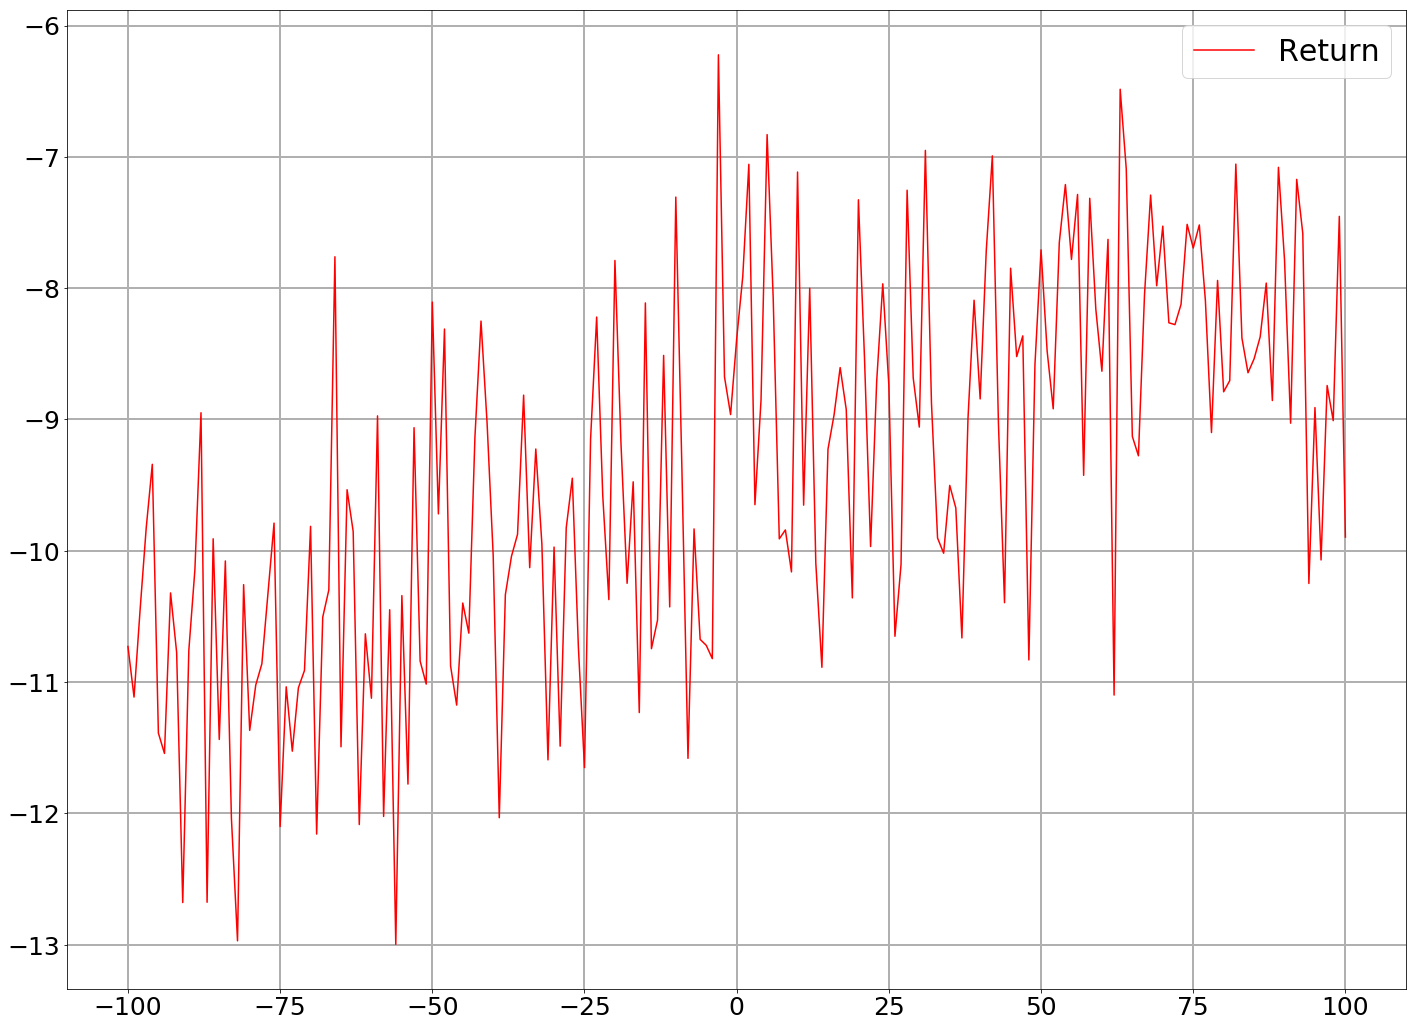
\includegraphics[width=\textwidth]{images/behaviour-up-10s-sell.png}
        \caption{Returns of sell orders within 10 seconds}
        \label{fig:behvaiour-up-10s-sell}
    \end{subfigure}
    \begin{subfigure}[b]{0.45\textwidth}
        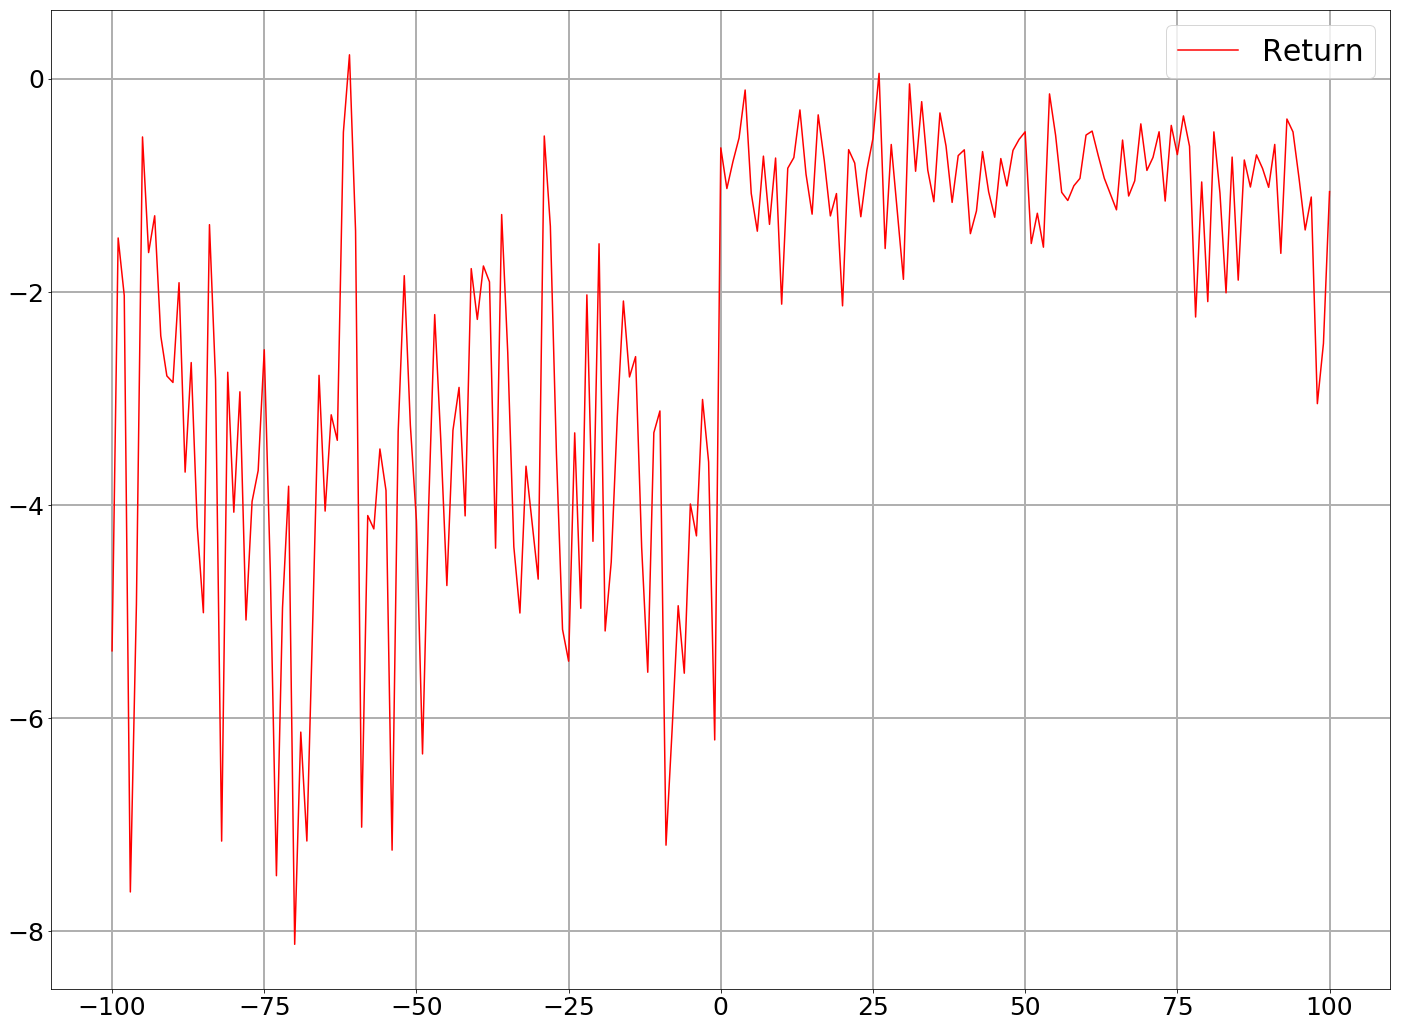
\includegraphics[width=\textwidth]{images/behaviour-up-30s-buy.png}
        \caption{Returns of buy orders within 30 seconds}
        \label{fig:behvaiour-up-30s-buy}
    \end{subfigure}
    \begin{subfigure}[b]{0.45\textwidth}
        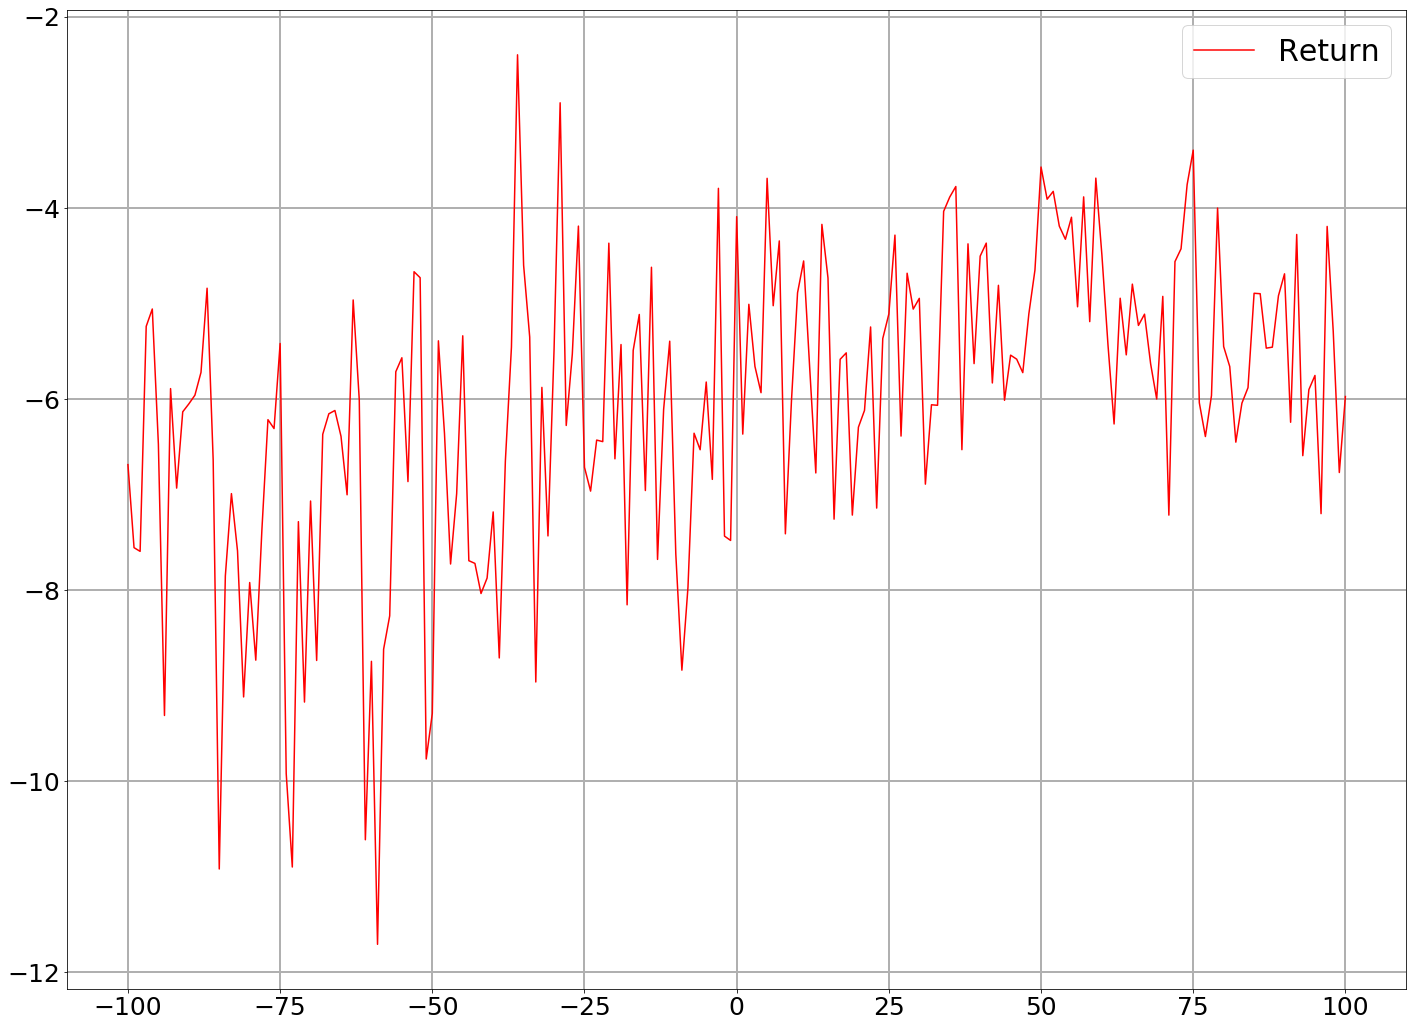
\includegraphics[width=\textwidth]{images/behaviour-up-30s-sell.png}
        \caption{Returns of sell orders within 30 seconds}
        \label{fig:behvaiour-up-30s-sell}
    \end{subfigure}
    \begin{subfigure}[b]{0.45\textwidth}
        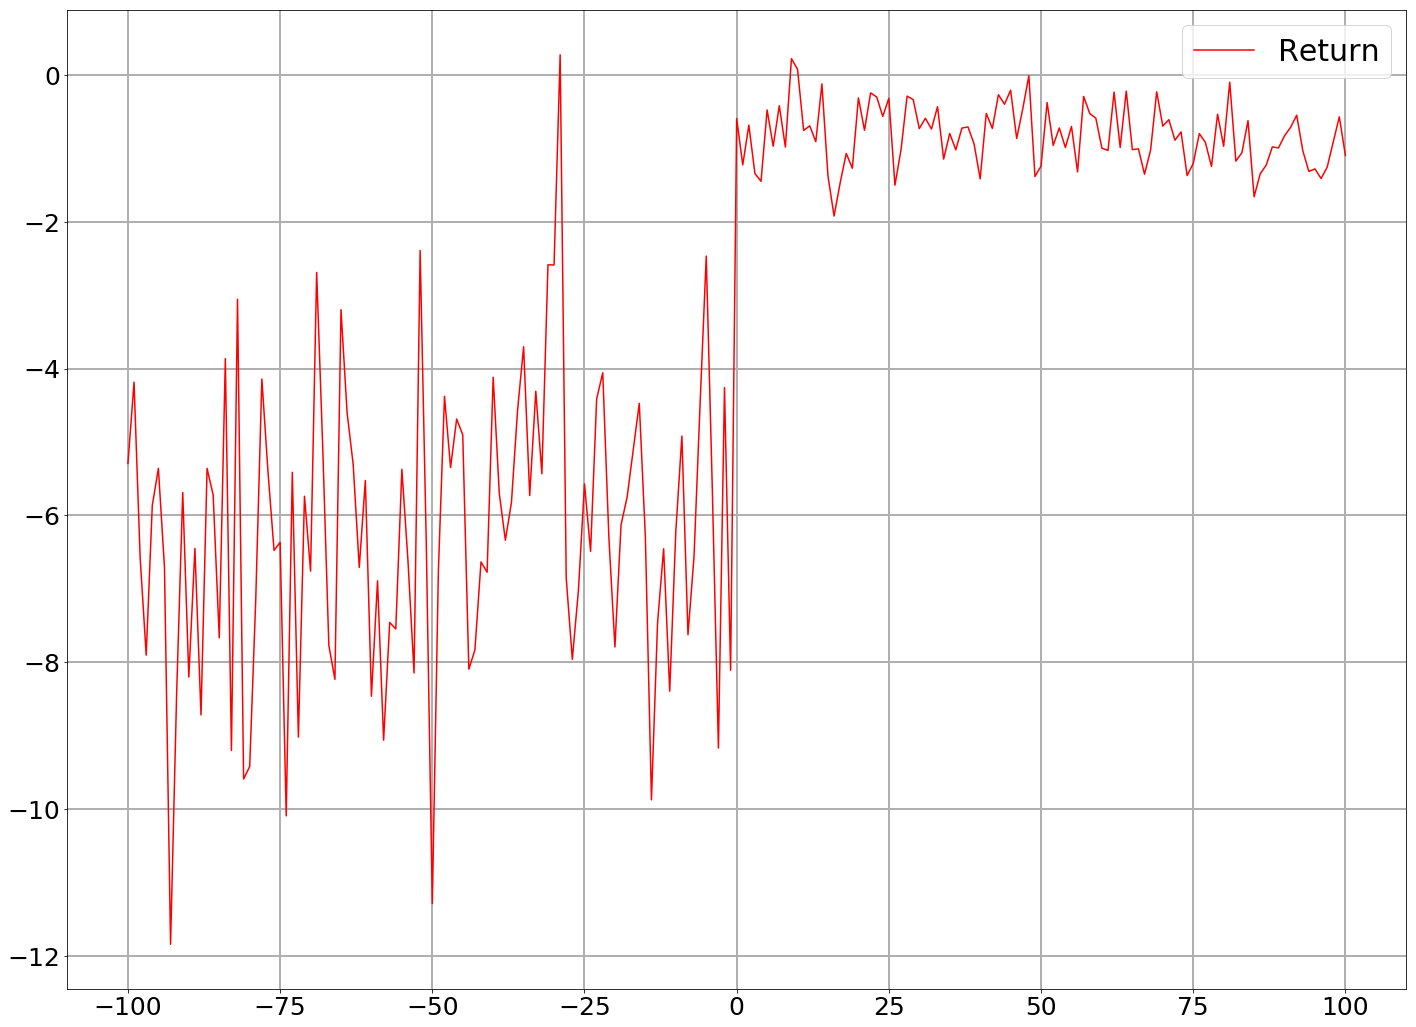
\includegraphics[width=\textwidth]{images/behaviour-up-60s-buy.png}
        \caption{Returns of buy orders within 60 seconds}
        \label{fig:behvaiour-up-60s-buy}
    \end{subfigure}
    \begin{subfigure}[b]{0.45\textwidth}
        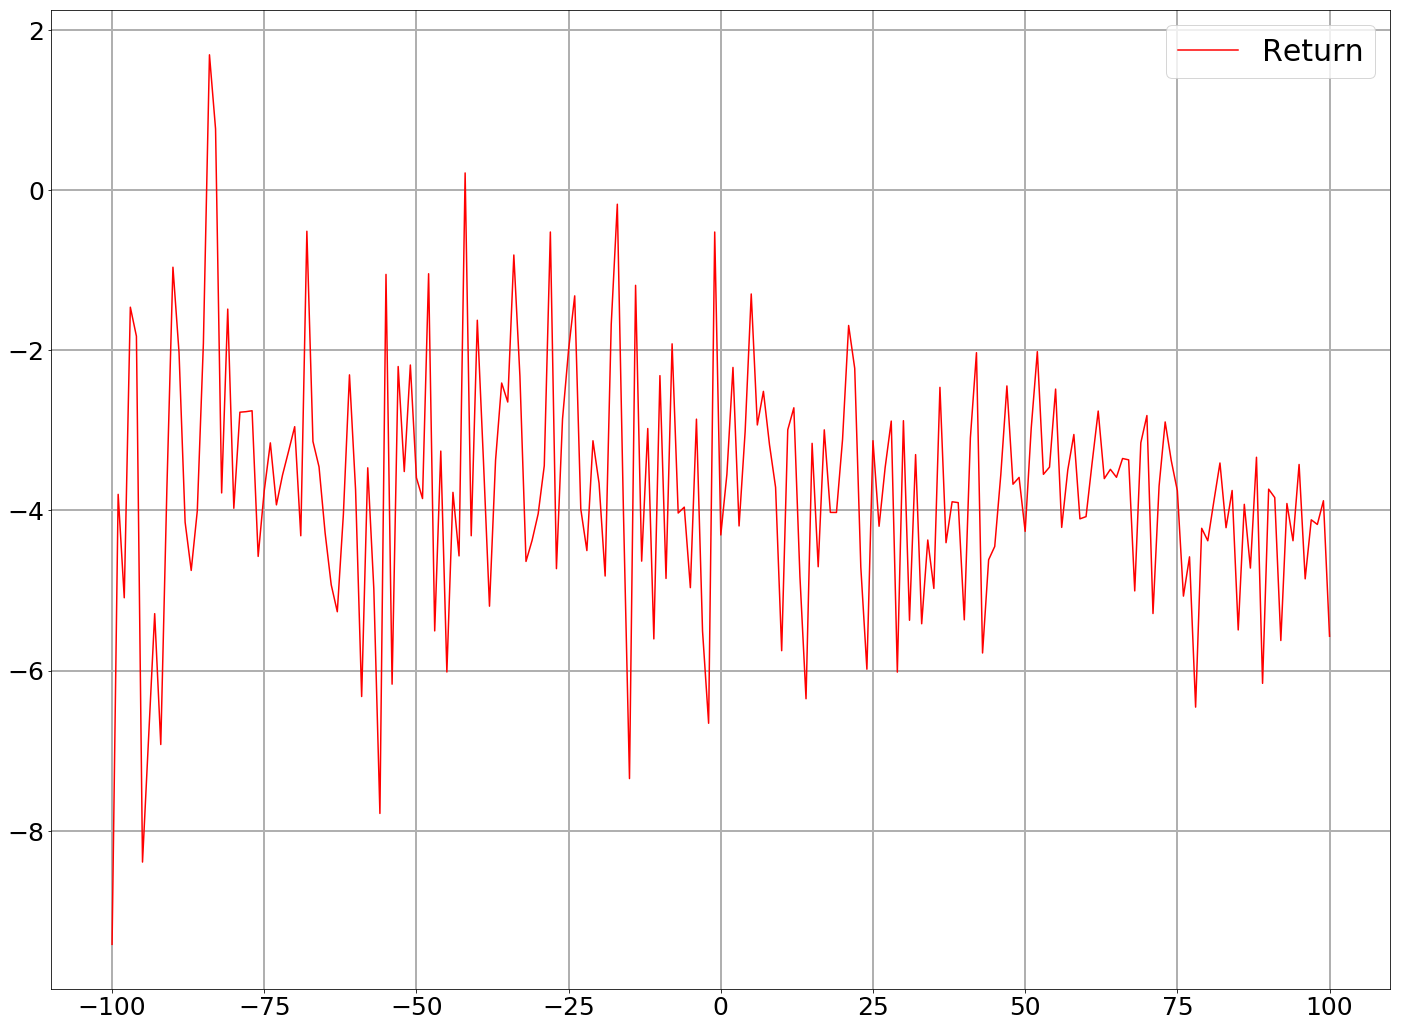
\includegraphics[width=\textwidth]{images/behaviour-up-60s-sell.png}
        \caption{Returns of sell orders 60 seconds}
        \label{fig:behvaiour-up-60s-sell}
    \end{subfigure}
    \begin{subfigure}[b]{0.45\textwidth}
        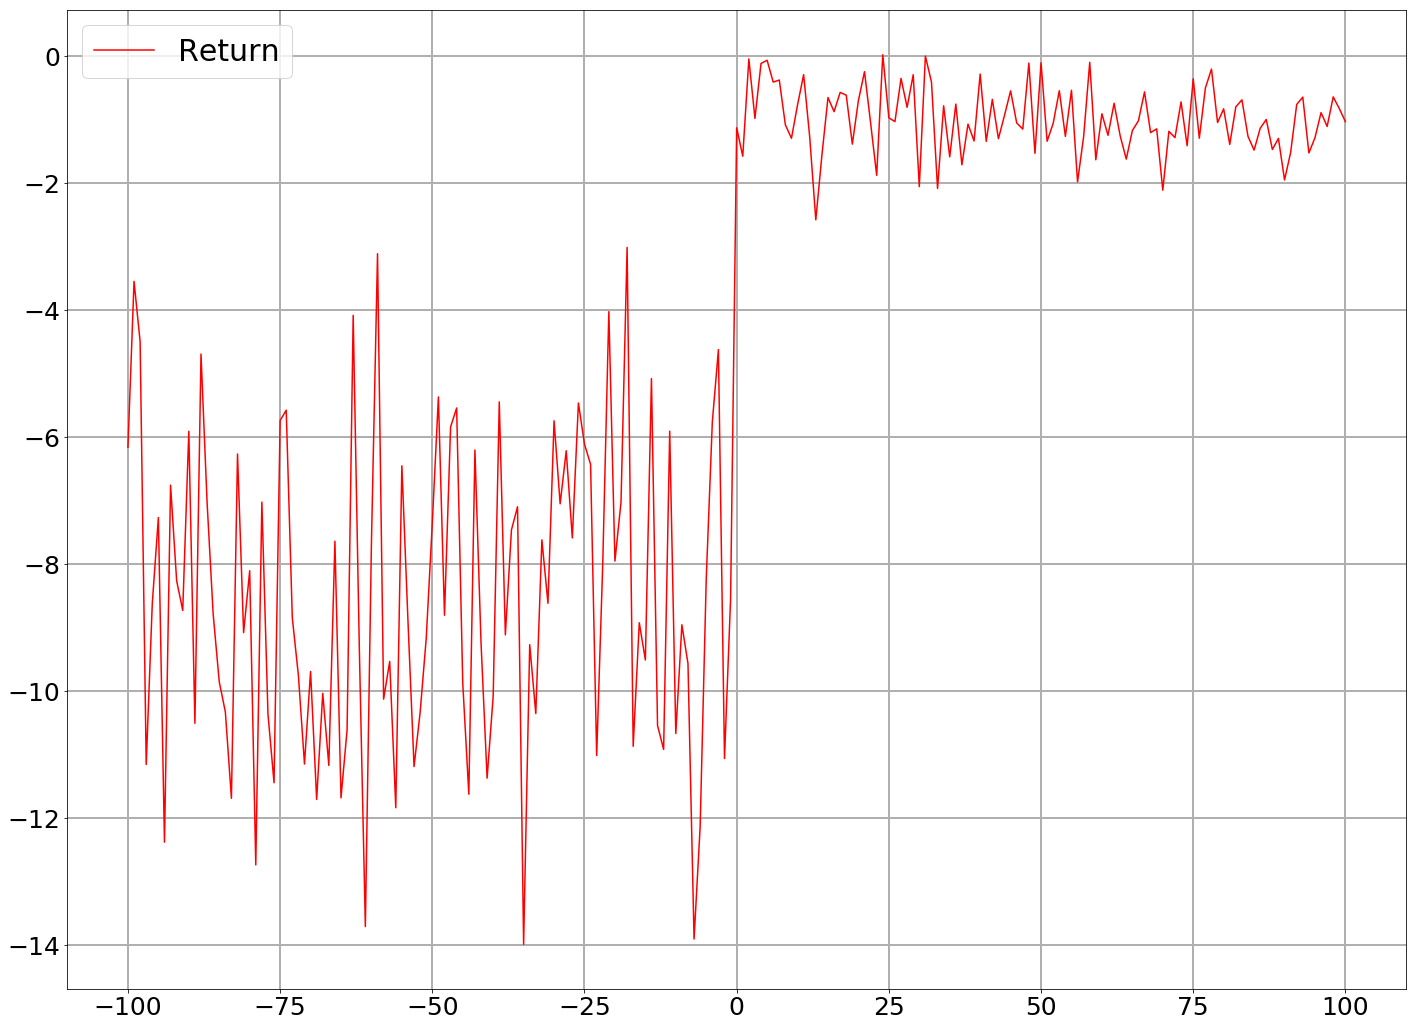
\includegraphics[width=\textwidth]{images/behaviour-up-100s-buy.png}
        \caption{Returns of buy orders 100 seconds}
        \label{fig:behvaiour-up-100s-buy}
    \end{subfigure}
    \begin{subfigure}[b]{0.45\textwidth}
        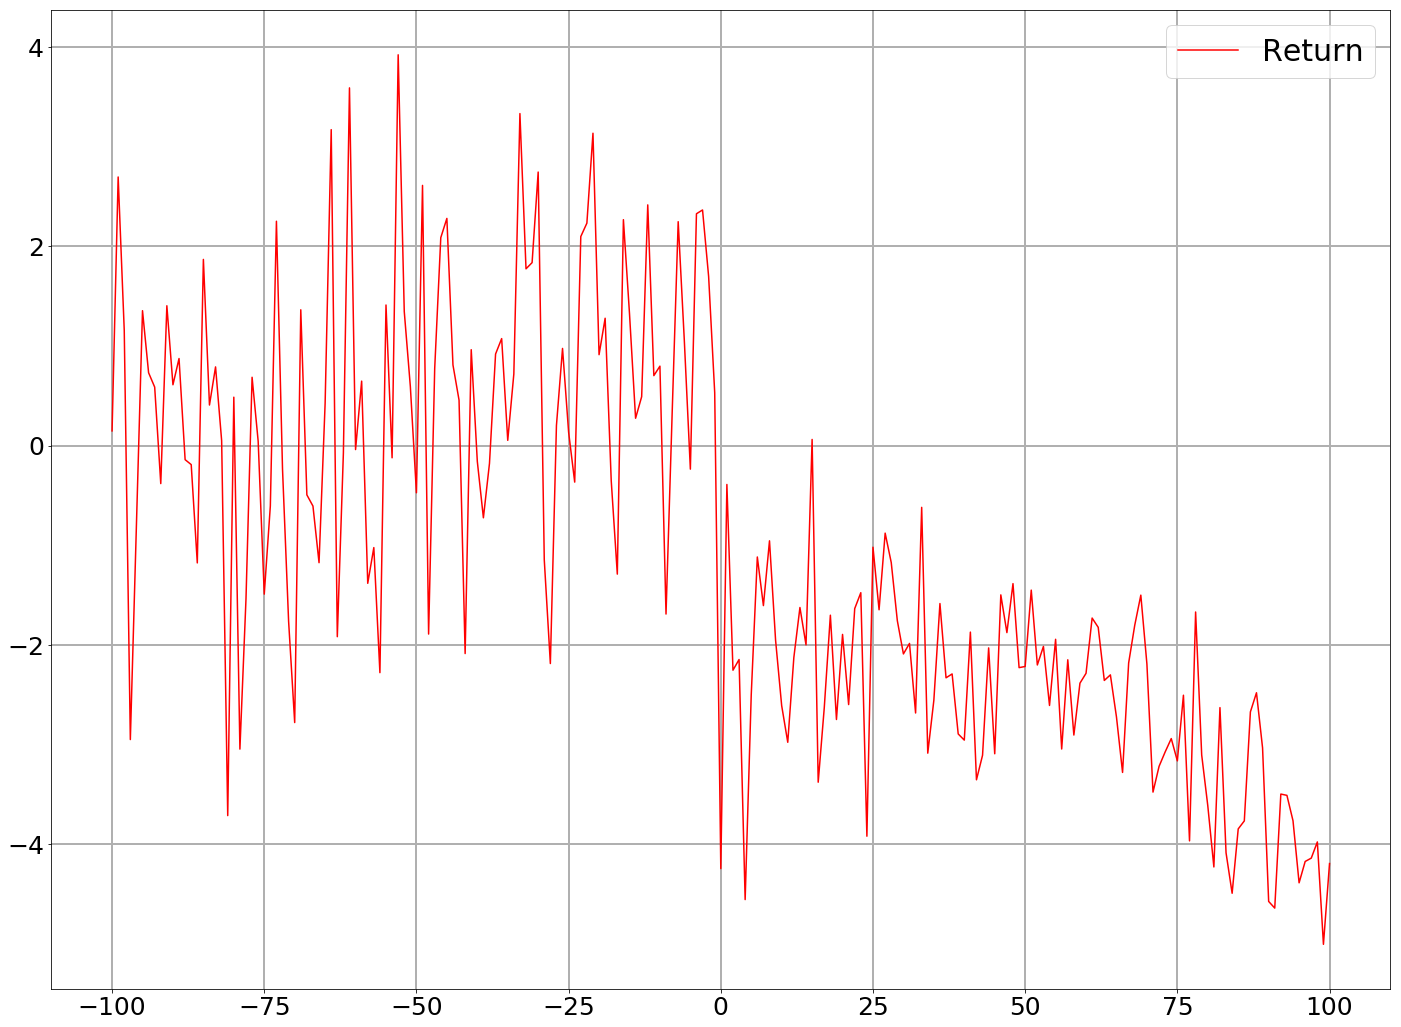
\includegraphics[width=\textwidth]{images/behaviour-up-100s-sell.png}
        \caption{Returns of sell orders 100 seconds}
        \label{fig:behvaiour-up-100s-sell}
    \end{subfigure}
    \caption{Returns of buy and sell orders executed within 10, 30, 60 and 100 seconds on data set II.}
    \label{fig:behvaiour-up}
\end{figure}

\subsection{Order placement behavior on data set II}
For the data set II, which shows an upwards price trend, the intuition is the opposite as for the investigation using data set I.
We expect buy orders to result in better returns when immediately filled, that is, when the agent crosses the spread and places the order high in the book ($a>0$).
The assumption is that, as time passes and the market price rises, other traders become less willing to sell for the market price or lower.
Therefore, the longer the time horizon given that is given to the agent, the more critical it becomes to execute immediately, as otherwise shares would have to be bought to an increased market price.
Contrarily, better returns with sell orders are expected when placed deep in the book ($a<0$), meaning to be sold at a higher price.
The assumption is that as the price rises, market participants become more likely to buy assets for higher prices.
Hence, the longer the time horizon, the deeper the agent should place a limit sell order in the book.
We investigate these assumptions by proceeding the same experiment as in the previous section, with time horizons of 10, 30, 60 and 100 seconds respectively, as shown in Figure \ref{fig:behvaiour-up}.

The returns of buy orders filled within a time horizon of 10 seconds, as shown in Figure \ref{fig:behvaiour-up-10s-buy}, correlate with the above stated assumptions.
The highest returns are achieved when crossing the spread and although limit levels in the range of 1-50 tend to perform the same, and considering the risk of paying a premium, the wisest choice for the agent would be to choose the level closest to the spread.
The sell orders placed with a time horizon of 10 seconds, contradict the assumptions, as shown in Figure \ref{fig:behvaiour-up-10s-sell}.
The agent is rewarded the most when choosing a price for the order at market price $a=0$.
A highly negative limit level causes to receive approximately \$3.00 less than when placing at the suggested market price.

With 30 seconds left to buy 1.0 BTC, in Figure \ref{fig:behvaiour-up-30s-buy}, the orders placed with $a>0$ (above the spread) become stable for any such limit level, much more so than with the same time horizon in the previous investigation with the data set I.
This is likely due to the higher order pressure of the data set II, as described in Section \ref{sec:analysis-data-sets}, as there are more market participants willing to sell.
The returns for limit sell orders, as shown in Figure \ref{fig:behvaiour-up-30s-sell}, become more rewarding as the agent benefits from a slight increase in price within the given time horizon.

This pattern becomes clearly apparent when a time horizon of 60 and 100 seconds was given, as shown in Figures \ref{fig:behvaiour-up-60s-sell} and \ref{fig:behvaiour-up-100s-sell} respectively.
With the increased time horizon, the assumptions stated in the beginning of this section are confirmed and the agent, when trying to sell shares, should indeed place orders deep in the order book ($a<0$).
As time passes and the market price rises, market participants are willing to buy for an increasing price and the agent is expected to be able to sell all assets for such an increased price without the need of a following market order.
Contrarily, if the agent decides to sell the assets for a decreasing price, as indicated by the higher limit levels, less reward can be expected with $a>0$.
More precisely, for a time horizon of 100 seconds, the agent is expected to receive up to \$7.00 less when choosing to cross the spread with a limit level of +100, compared to some negative limit level.
Figures \ref{fig:behvaiour-up-60s-buy} and \ref{fig:behvaiour-up-100s-buy} which show the expected results of an agent that buys assets within the 60 and 100 seconds respectively.
As is evident, this uprising market price determines that the expected damage can be minimized by crossing the spread and buying immediately.
The advice stated before remains: the agent should choose a price slightly above the market price as there is enough liquidity in the market to buy the demanded number of assets.

\subsection{Conclusion of empirical analysis}
The results of the empirical analysis proceeded on data set I and II have shown that the tendency of limit order placement is as follows:
during a downwards trend of the market price, buying assets can be optimized by placing limit orders deep in the order book ($a<0$) and the least loss is taken when selling assets immediately to the market price ($a>0$).
Contrarily, during an upwards market price trend, buying assets is suggested using a market order ($a>0$) and selling can be optimized by placing the sell orders deep in the order book ($a<0$).
This effect becomes more apparent when a longer time horizon is given for an order, as for shorter time horizons the order placement process gets either intercepted by short term fluctuations or a lack of market participants providing volume to buy and sell assets.
The latter implies that, during an upwards trend, market participants are willing to buy and sell shares for higher prices and contrarily, during a downwards trend for lower prices.
In this analysis, the orders placed had to be completely filled without the ability to make intermediary steps of cancellations and replacements of the order within the given time horizon.
It is therefore to be evaluated by the reinforcement learners whether or not such adaptions to the order will result in a more favorable reward.
In order to have a measure of comparison for the reinforcement learning agents to come, Table \ref{tbl:analysis-empirical-summary} summarizes the findings and shows the expected rewards for (1) the optimal limit level chosen and (2) an immediate completion of the order using a market order.
\begin{table}[H]
\centering
\begin{tabular}{l|l|l|}
\cline{2-3}
& \textbf{$\mathbb{E}$[Limit order] (optimal)} & \textbf{\begin{tabular}[c]{@{}l@{}}$\mathbb{E}$[Market order]\end{tabular}} \\ \hline
\multicolumn{1}{|l|}{\textbf{Buy (I)}}   & 15.20          & -0.05                                                           \\ \hline
\multicolumn{1}{|l|}{\textbf{Sell (I)}}  & -27.70         & -27.70                                                          \\ \hline
\multicolumn{1}{|l|}{\textbf{Buy (II)}}  & -1.06          & -1.06                                                           \\ \hline
\multicolumn{1}{|l|}{\textbf{Sell (II)}} & 3.68          & -1.72                                                           \\ \hline
\end{tabular}
\caption{Summary of rewards derived form the empirical analysis.}
\label{tbl:analysis-empirical-summary}
\end{table}

\section{Q-Learning without market variables}
\label{sec:eval-qlearn}
The previous section provided knowledge about the expected rewards an agent will receive when placing buy and sell orders using the reinforcement learning environment and with the underlying data set I and II.
For each such observation, a fixed time horizon was chosen for which an order was placed in the order book, followed by a market order in case the order has not been filled completely.

This section aims to investigate whether or not a Q-Learning agent, as described in Chapter \ref{chap:setup} (Section \ref{setup:q-learning}), can improve the received rewards over the expected return for a market order as derived in the previous section.
Thereby, the agent is allowed to cancel its order after every 10 seconds and place a new order with the remaining inventory (e.g. $\Delta{t}=10$), until the time horizon of 100 seconds is fully consumed.
After which, and in case the order has not been filled completely, a market order follows for the remaining share to be bought or sold.
For both data sets (I and II) an independent learning experiment is being proceeded where the agent is supposed to either buy or sell shares.
For each such experiment, the training is limited to 5000 epochs and 1000 orders are being placed and evaluated on the test set (denoted as "backtesting").
The Q-Learning agent is set up as follows:
the learning rate $\alpha=0.1$ is chosen small due to extensive amounts of steps the agent will make throughout the epochs.
The discount factor $\gamma=0.5$ is chosen to balance the agents incentive to profit from immediate rewards and consuming the entirety of the given time horizon.
Initially, the exploration constant $\epsilon$ is set to 0.8 and a decay is applied such that the factor reduces to $\epsilon=0.1$ by the time the training is completed.
This allows the agent first to explore the action space and then exploit on the learned optimal actions to take.

With this setup, four observations were made and for each of which the training and testing results are stated below.
During training, the mean rewards and the average action chosen for each epoch, were recorded.
Once the model was trained, a backtest was run on the test data sets where the agent executed orders by choosing from the learned optimal actions.

\subsection{Results of training and testing on data set I and II}

\begin{figure}
    \centering
    \begin{subfigure}[b]{0.4\textwidth}
        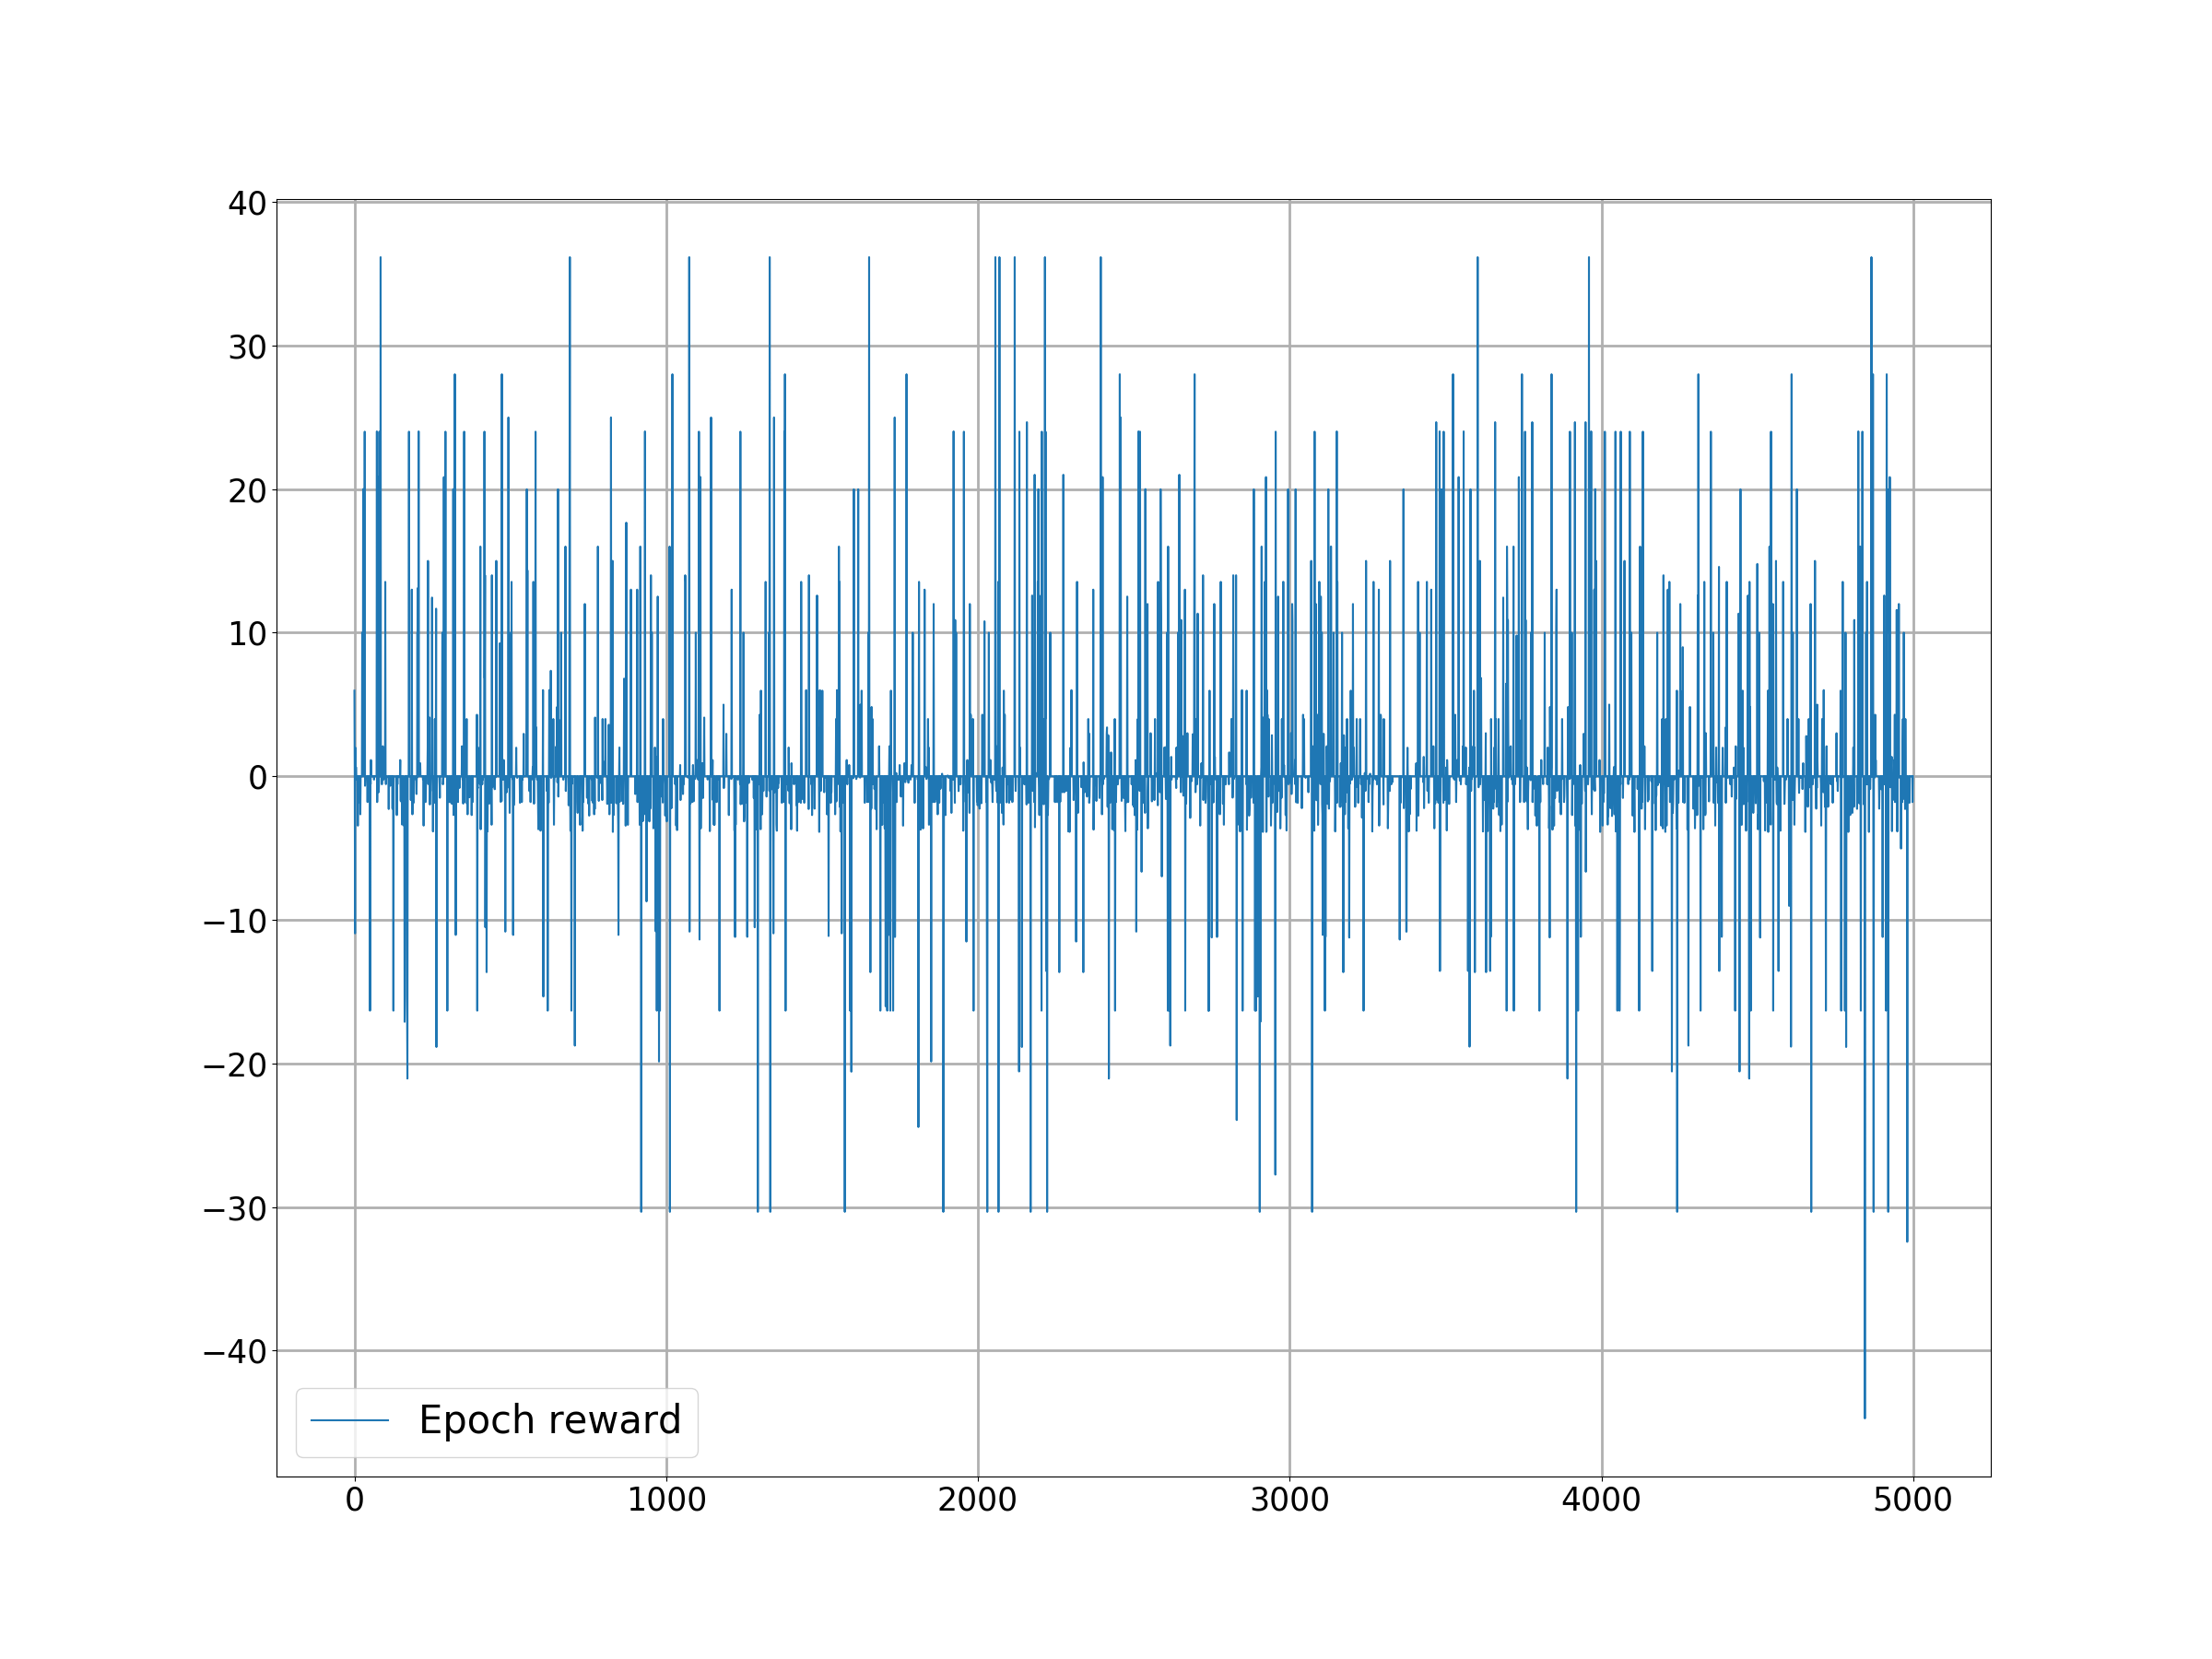
\includegraphics[width=\textwidth]{q_1_10000_BUY_rewards.png}
        \caption{Mean rewards per epoch (buy)}
        \label{fig:analysis-q-learn-1-reward-buy}
    \end{subfigure}
    \begin{subfigure}[b]{0.4\textwidth}
        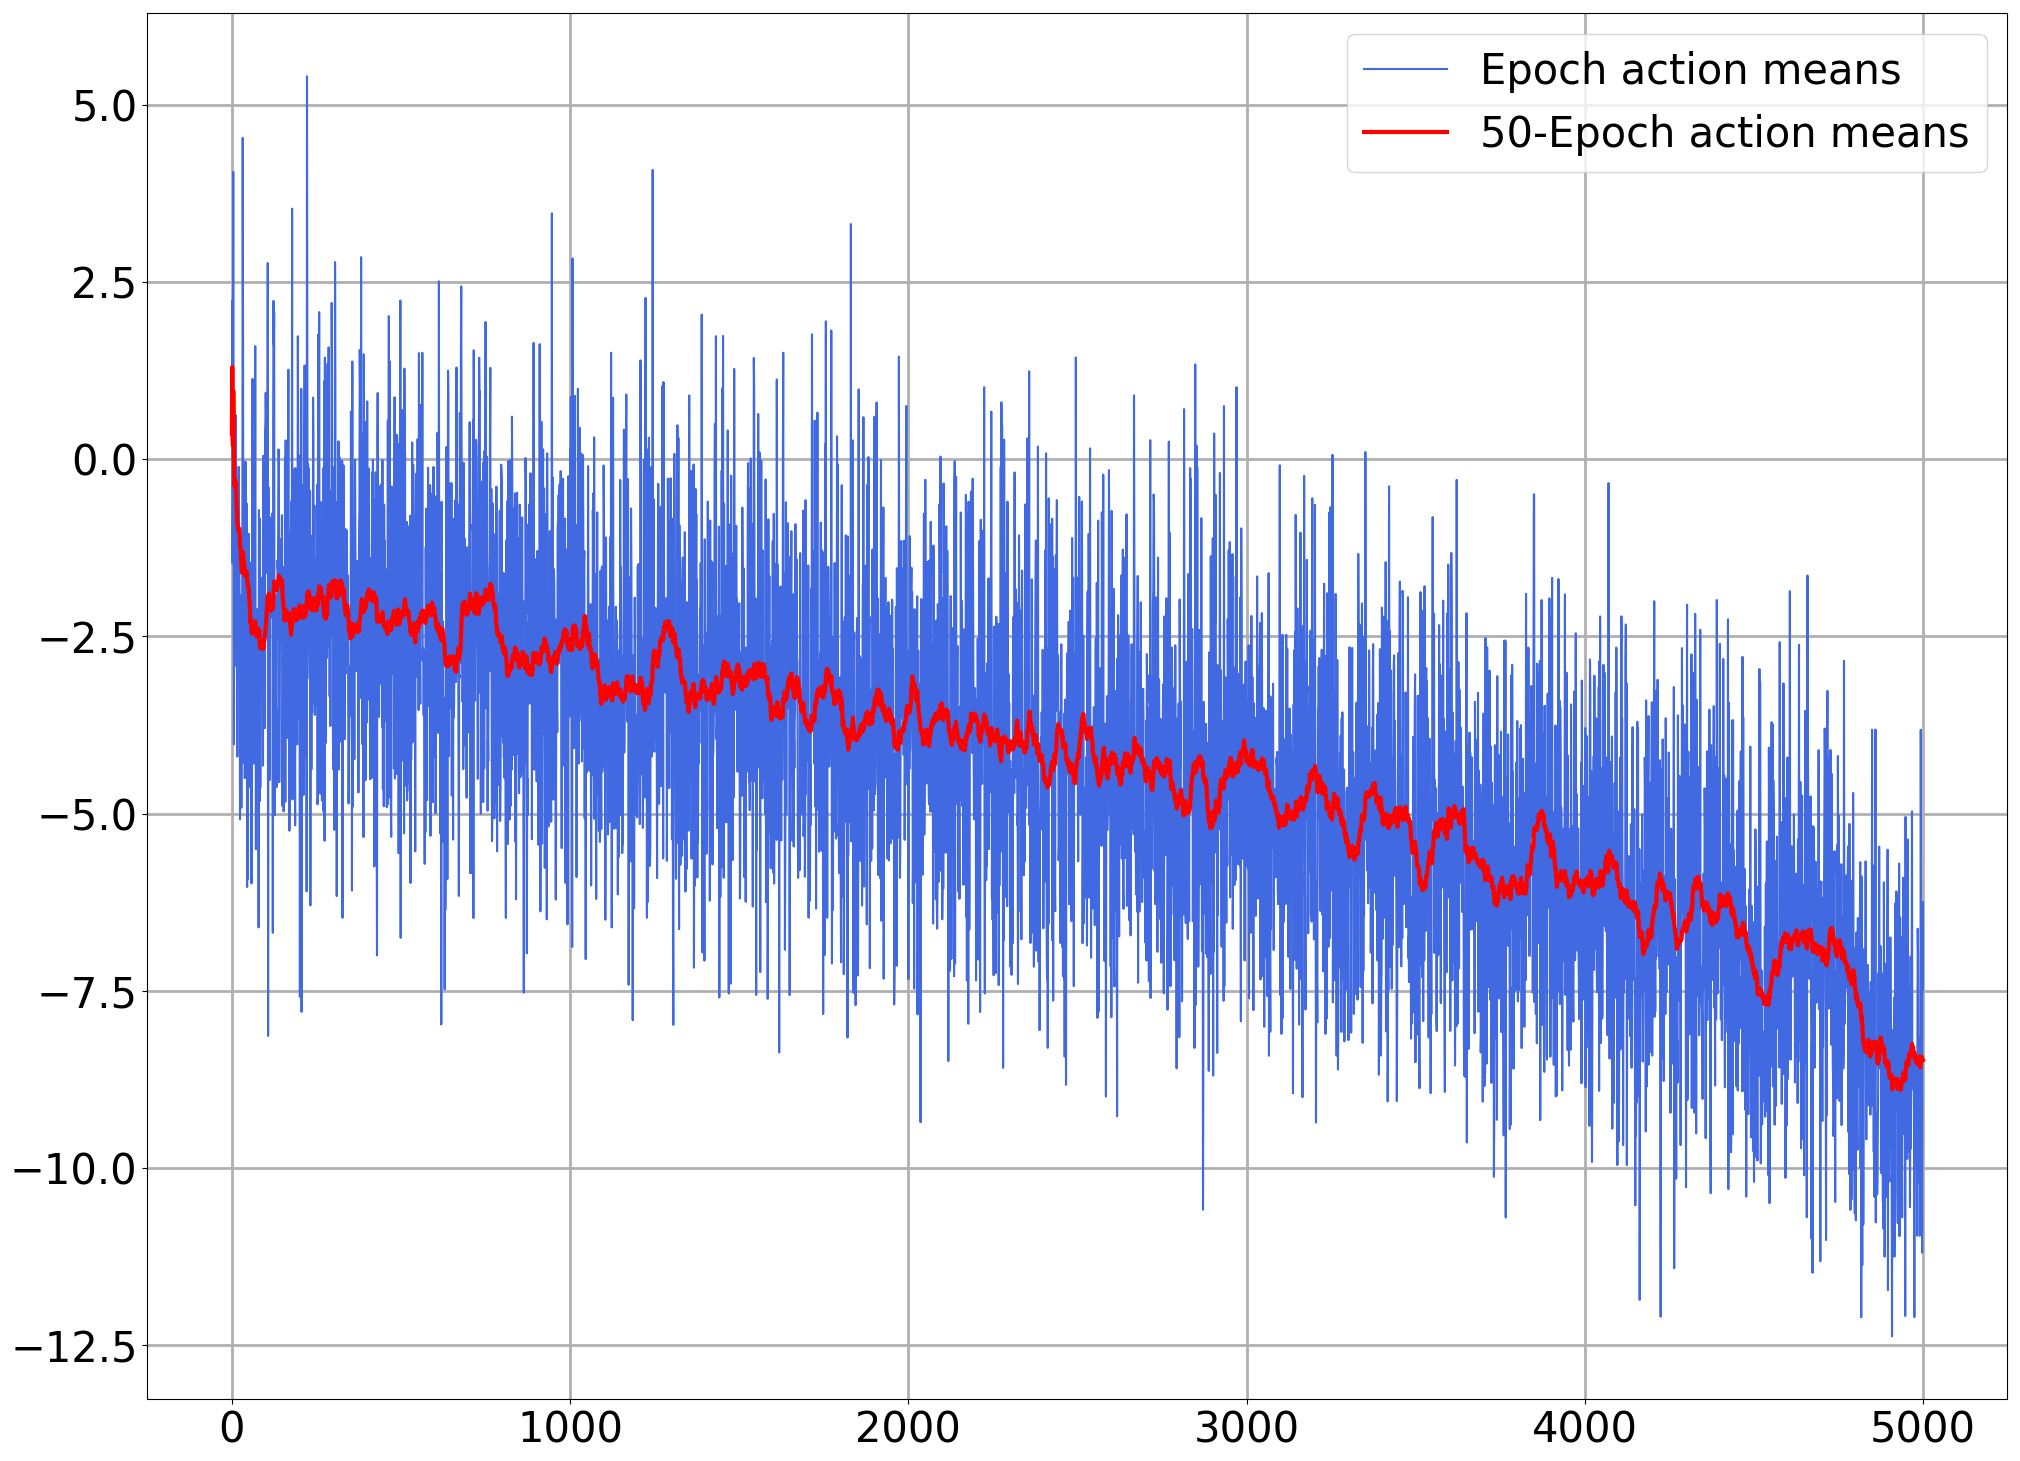
\includegraphics[width=\textwidth]{q_1_10000_BUY_mean_actions.png}
        \caption{Mean of actions per epoch (buy)}
        \label{fig:analysis-q-learn-1-action-buy}
    \end{subfigure}
    \begin{subfigure}[b]{0.4\textwidth}
        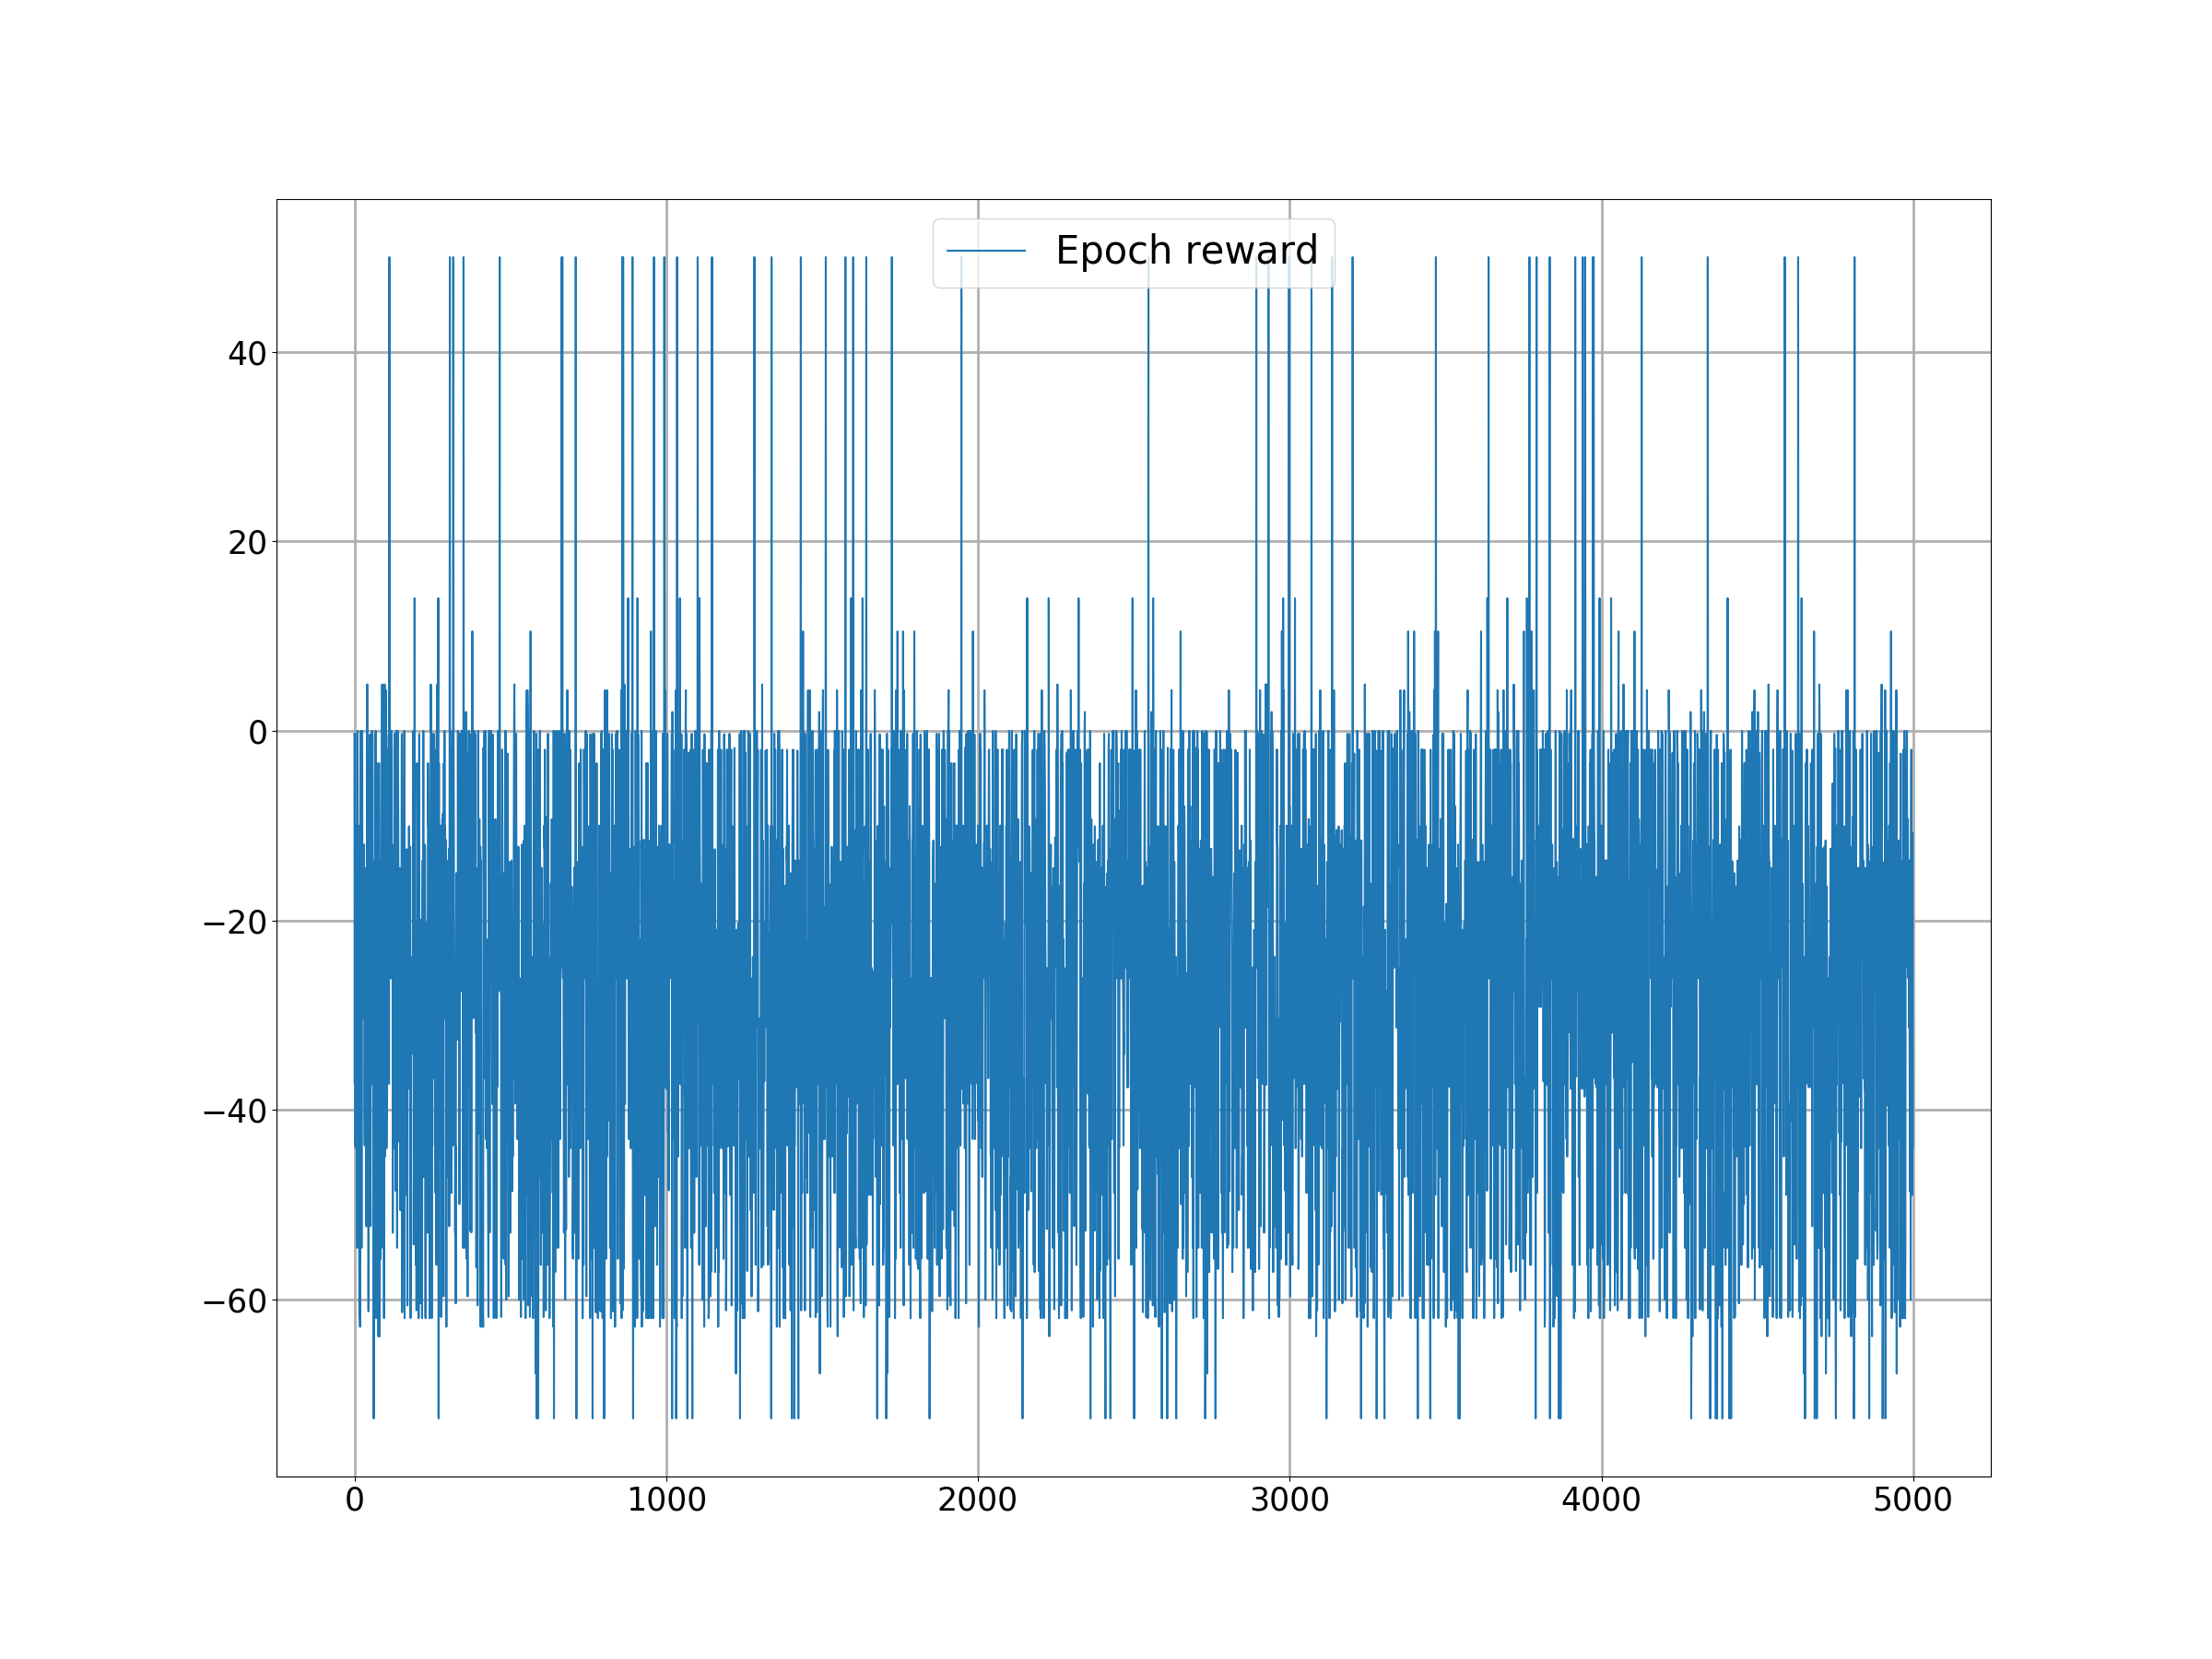
\includegraphics[width=\textwidth]{q_1_10000_SELL_rewards.png}
        \caption{Mean rewards per epoch (sell)}
        \label{fig:analysis-q-learn-1-reward-sell}
    \end{subfigure}
    \begin{subfigure}[b]{0.4\textwidth}
        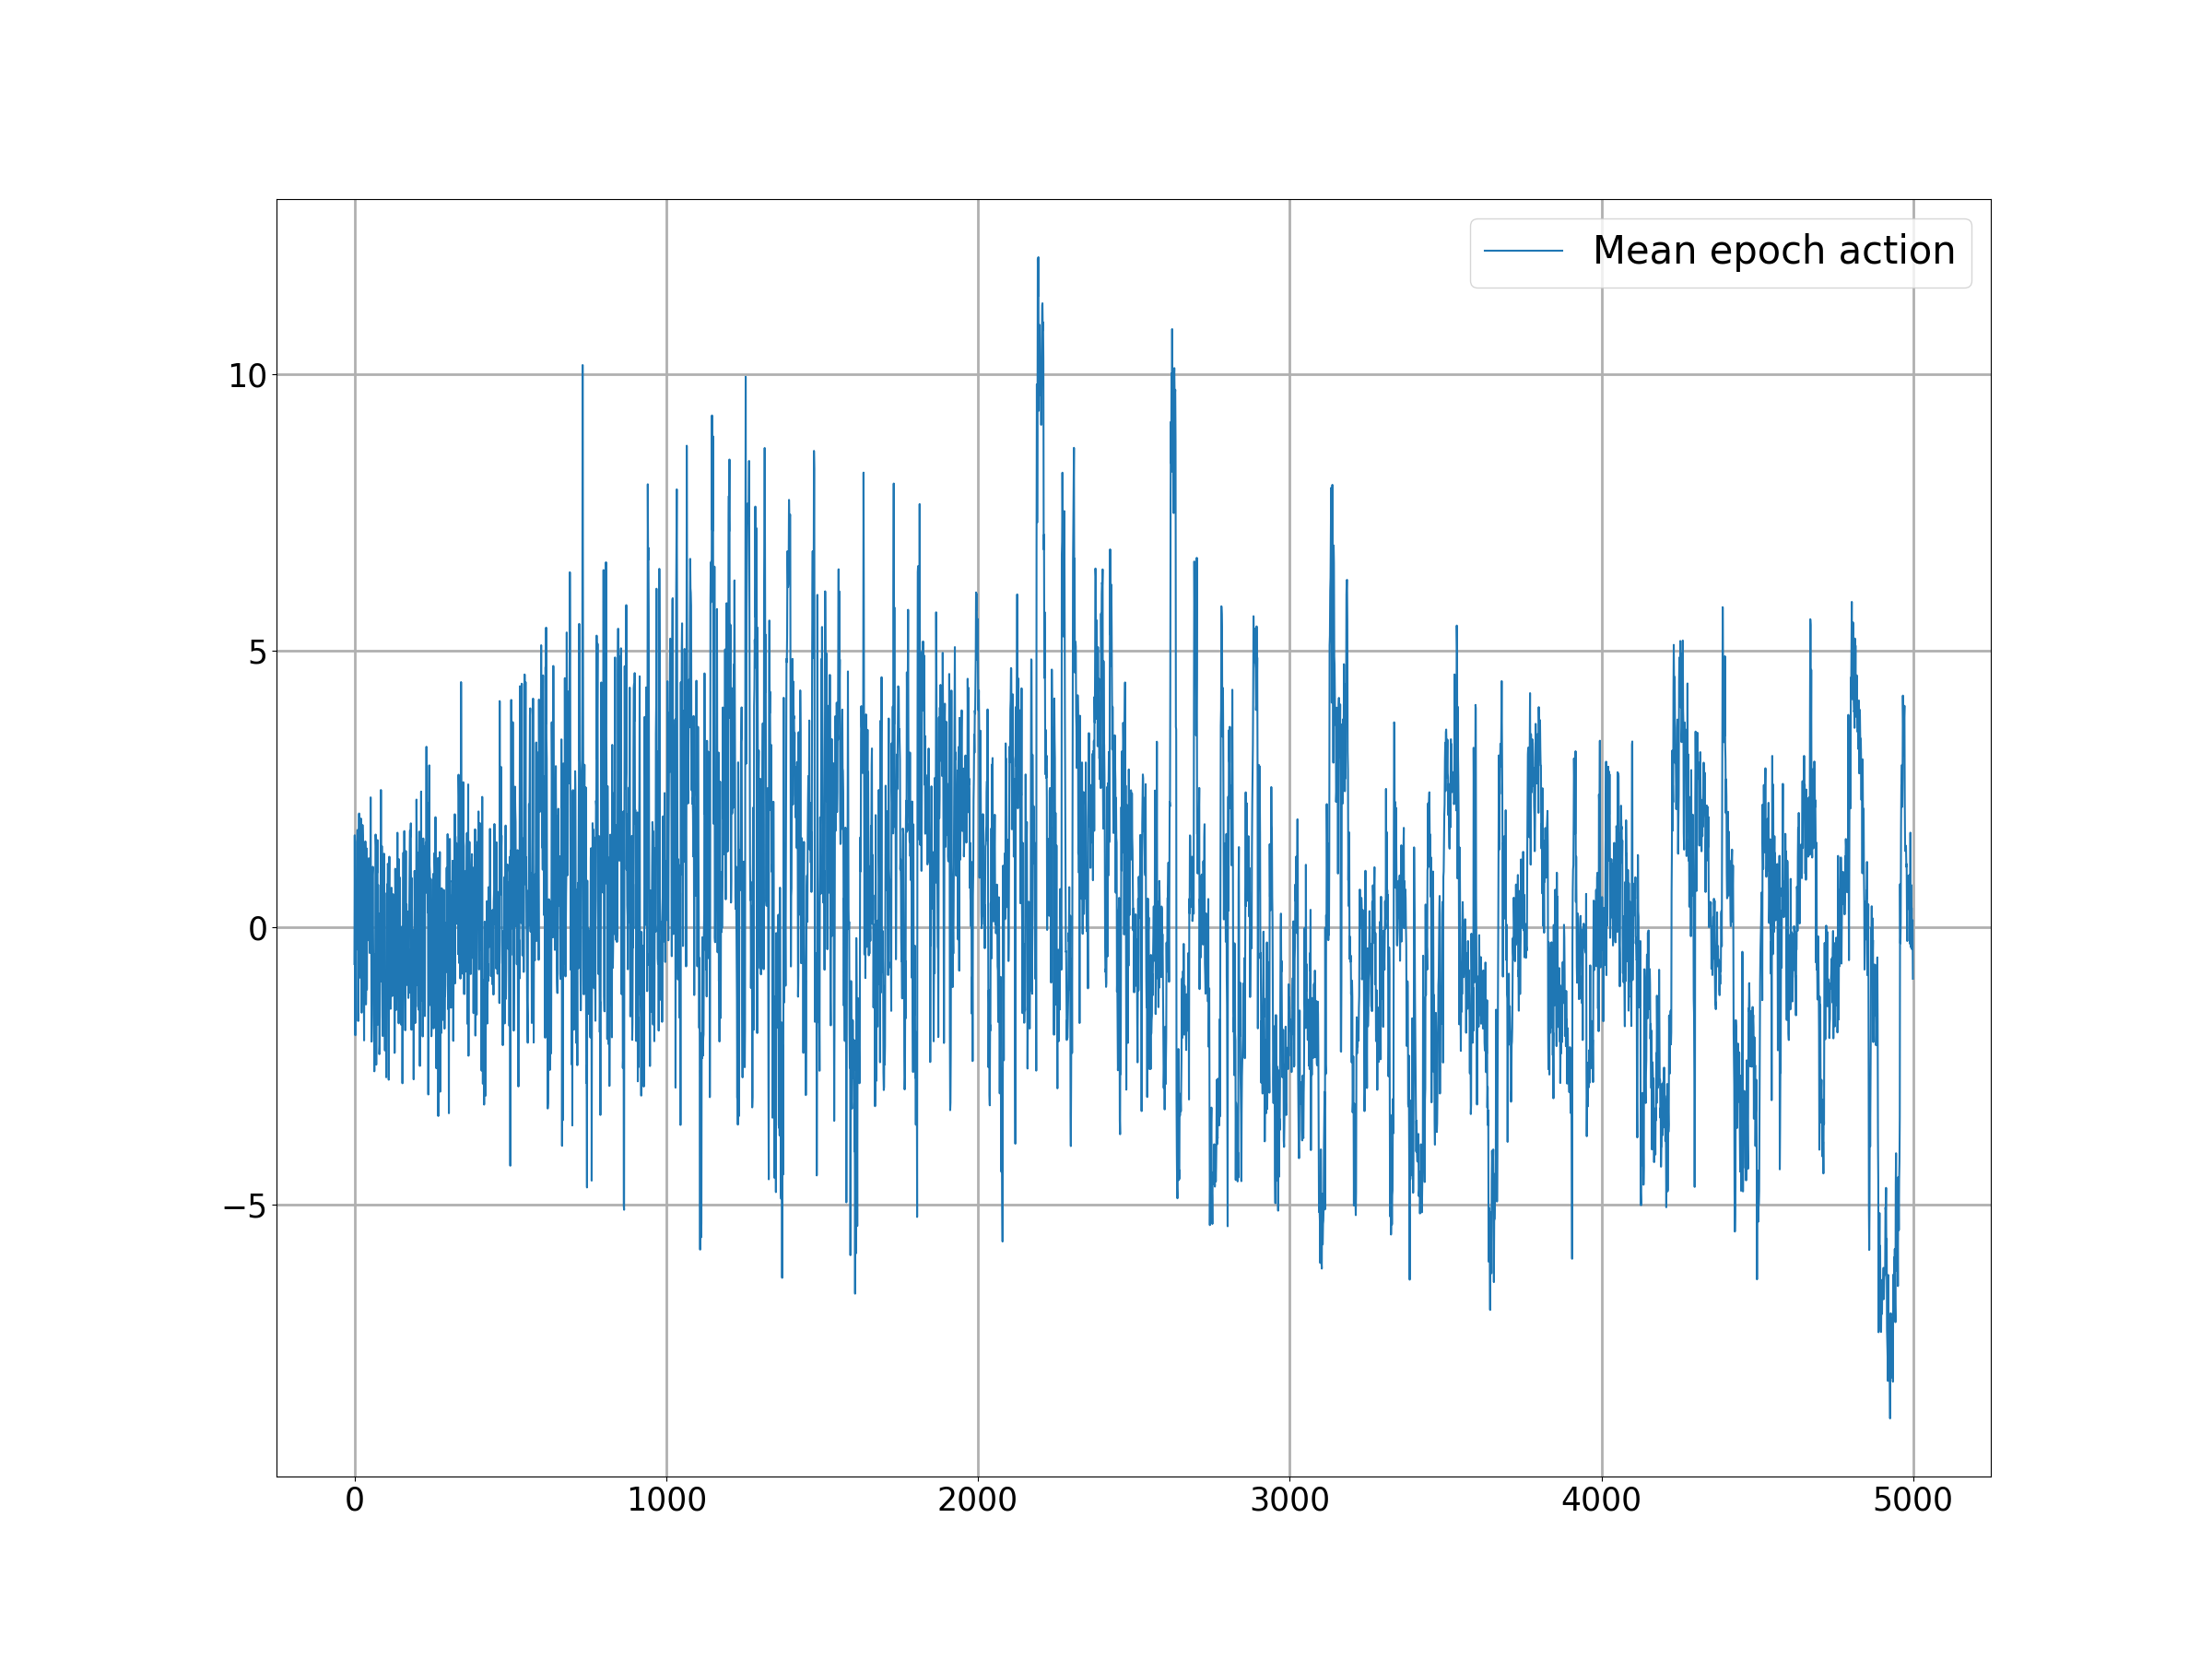
\includegraphics[width=\textwidth]{q_1_10000_SELL_mean_actions.png}
        \caption{Mean of actions per epoch (sell)}
        \label{fig:analysis-q-learn-1-action-sell}
    \end{subfigure}
    \caption{Mean rewards and actions for buying and selling on training data set I.}
    \label{fig:analysis-q-learn-1}
\end{figure}
\begin{figure}
    \centering
    \begin{subfigure}[b]{0.4\textwidth}
        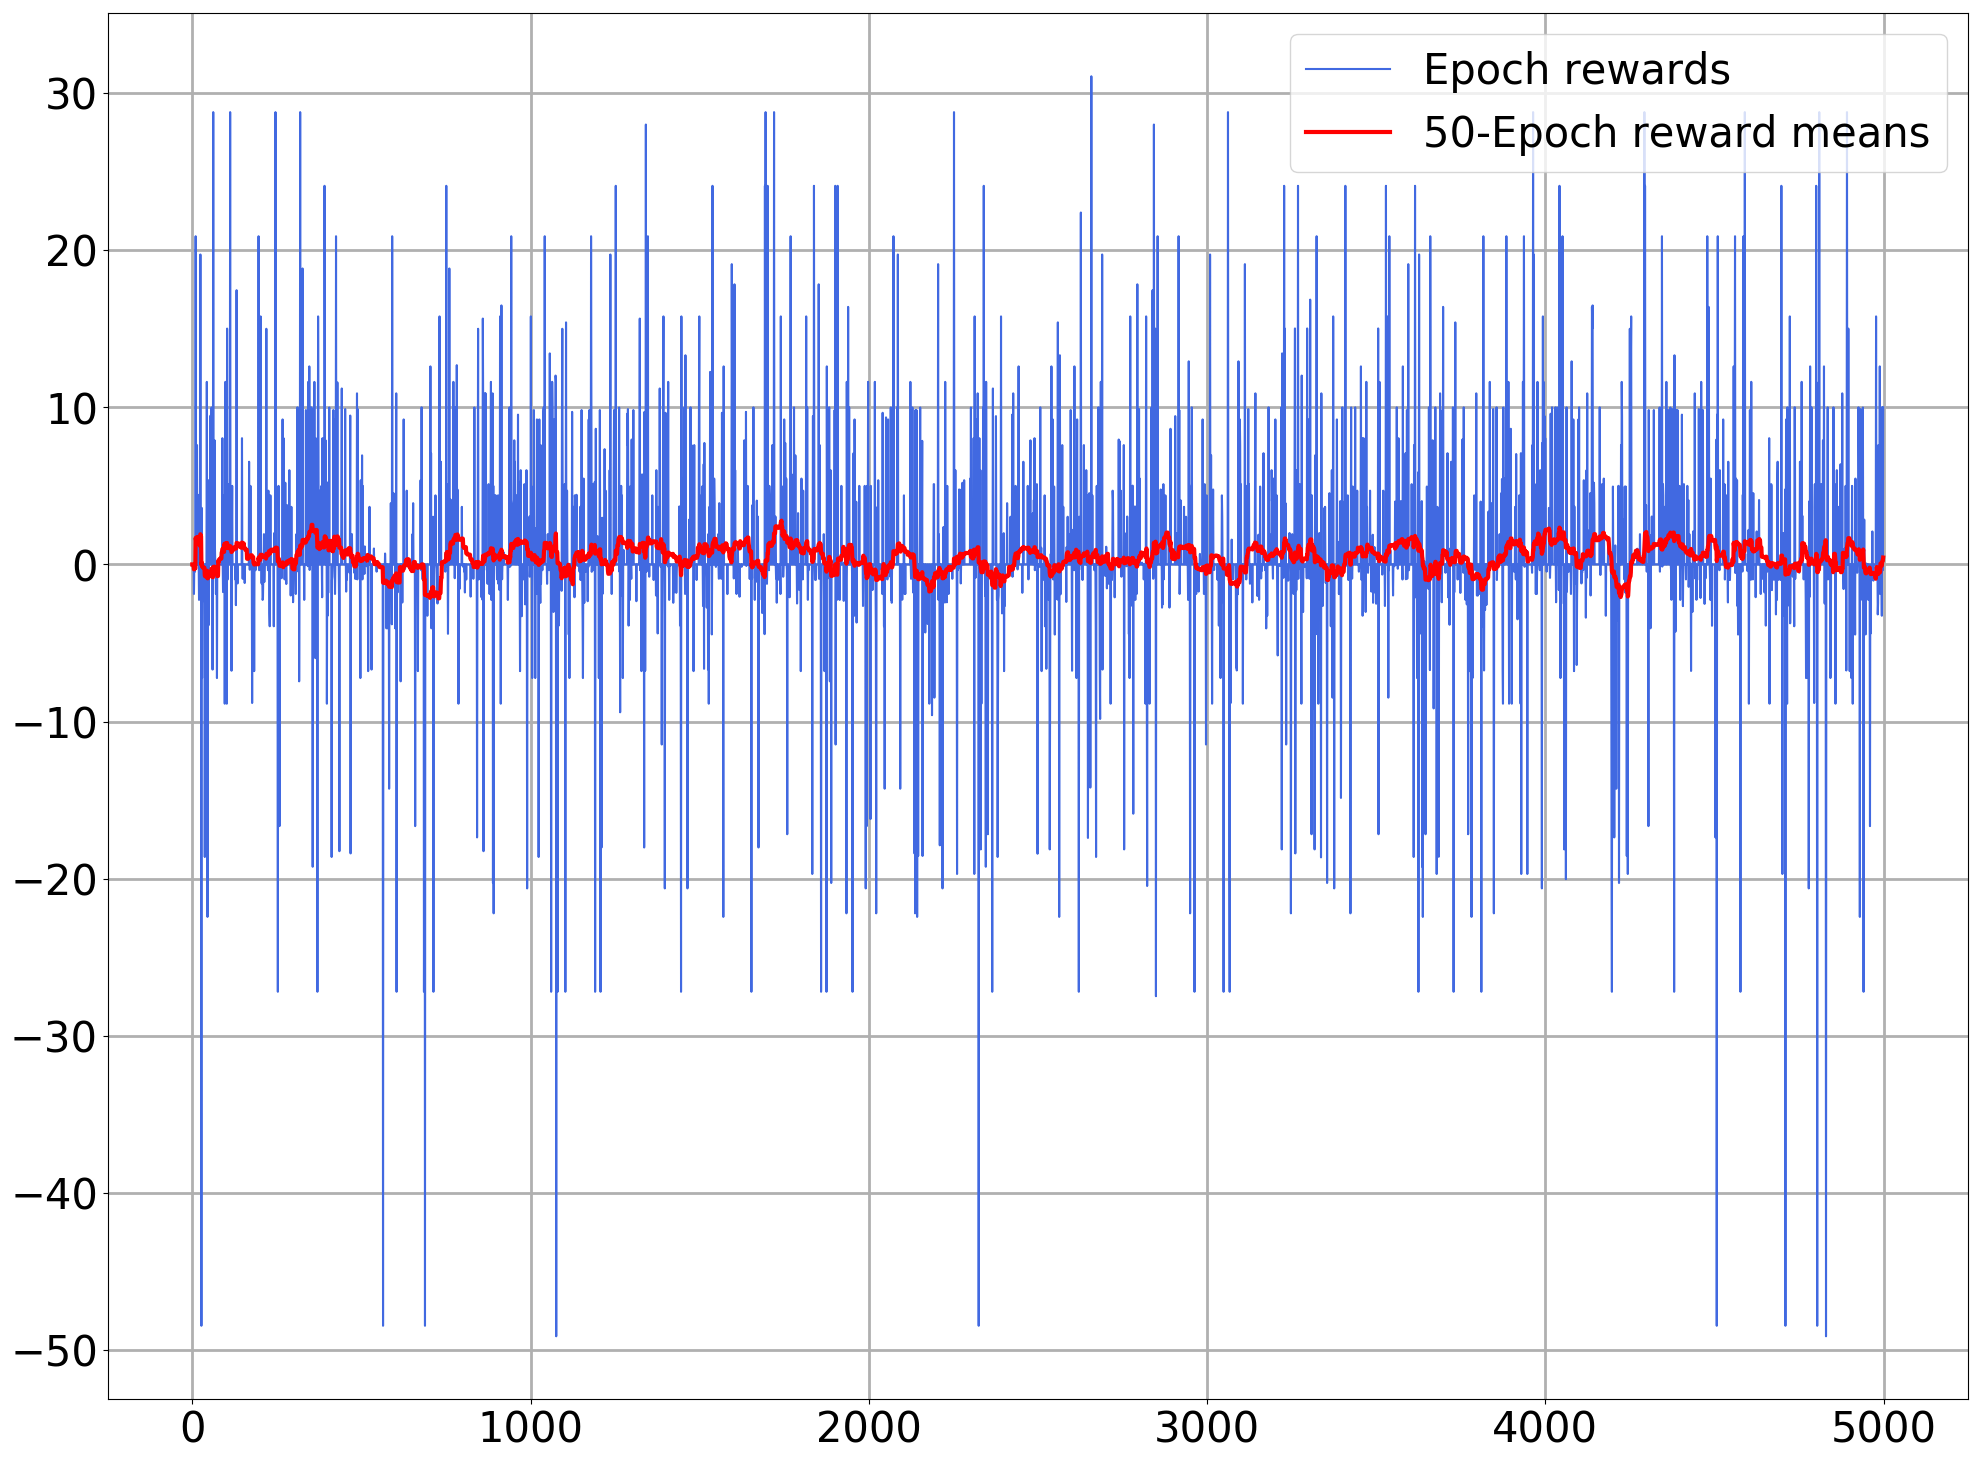
\includegraphics[width=\textwidth]{q_2_10000_BUY_rewards.png}
        \caption{Mean rewards per epoch (buy)}
        \label{fig:analysis-q-learn-2-reward-buy}
    \end{subfigure}
    \begin{subfigure}[b]{0.4\textwidth}
        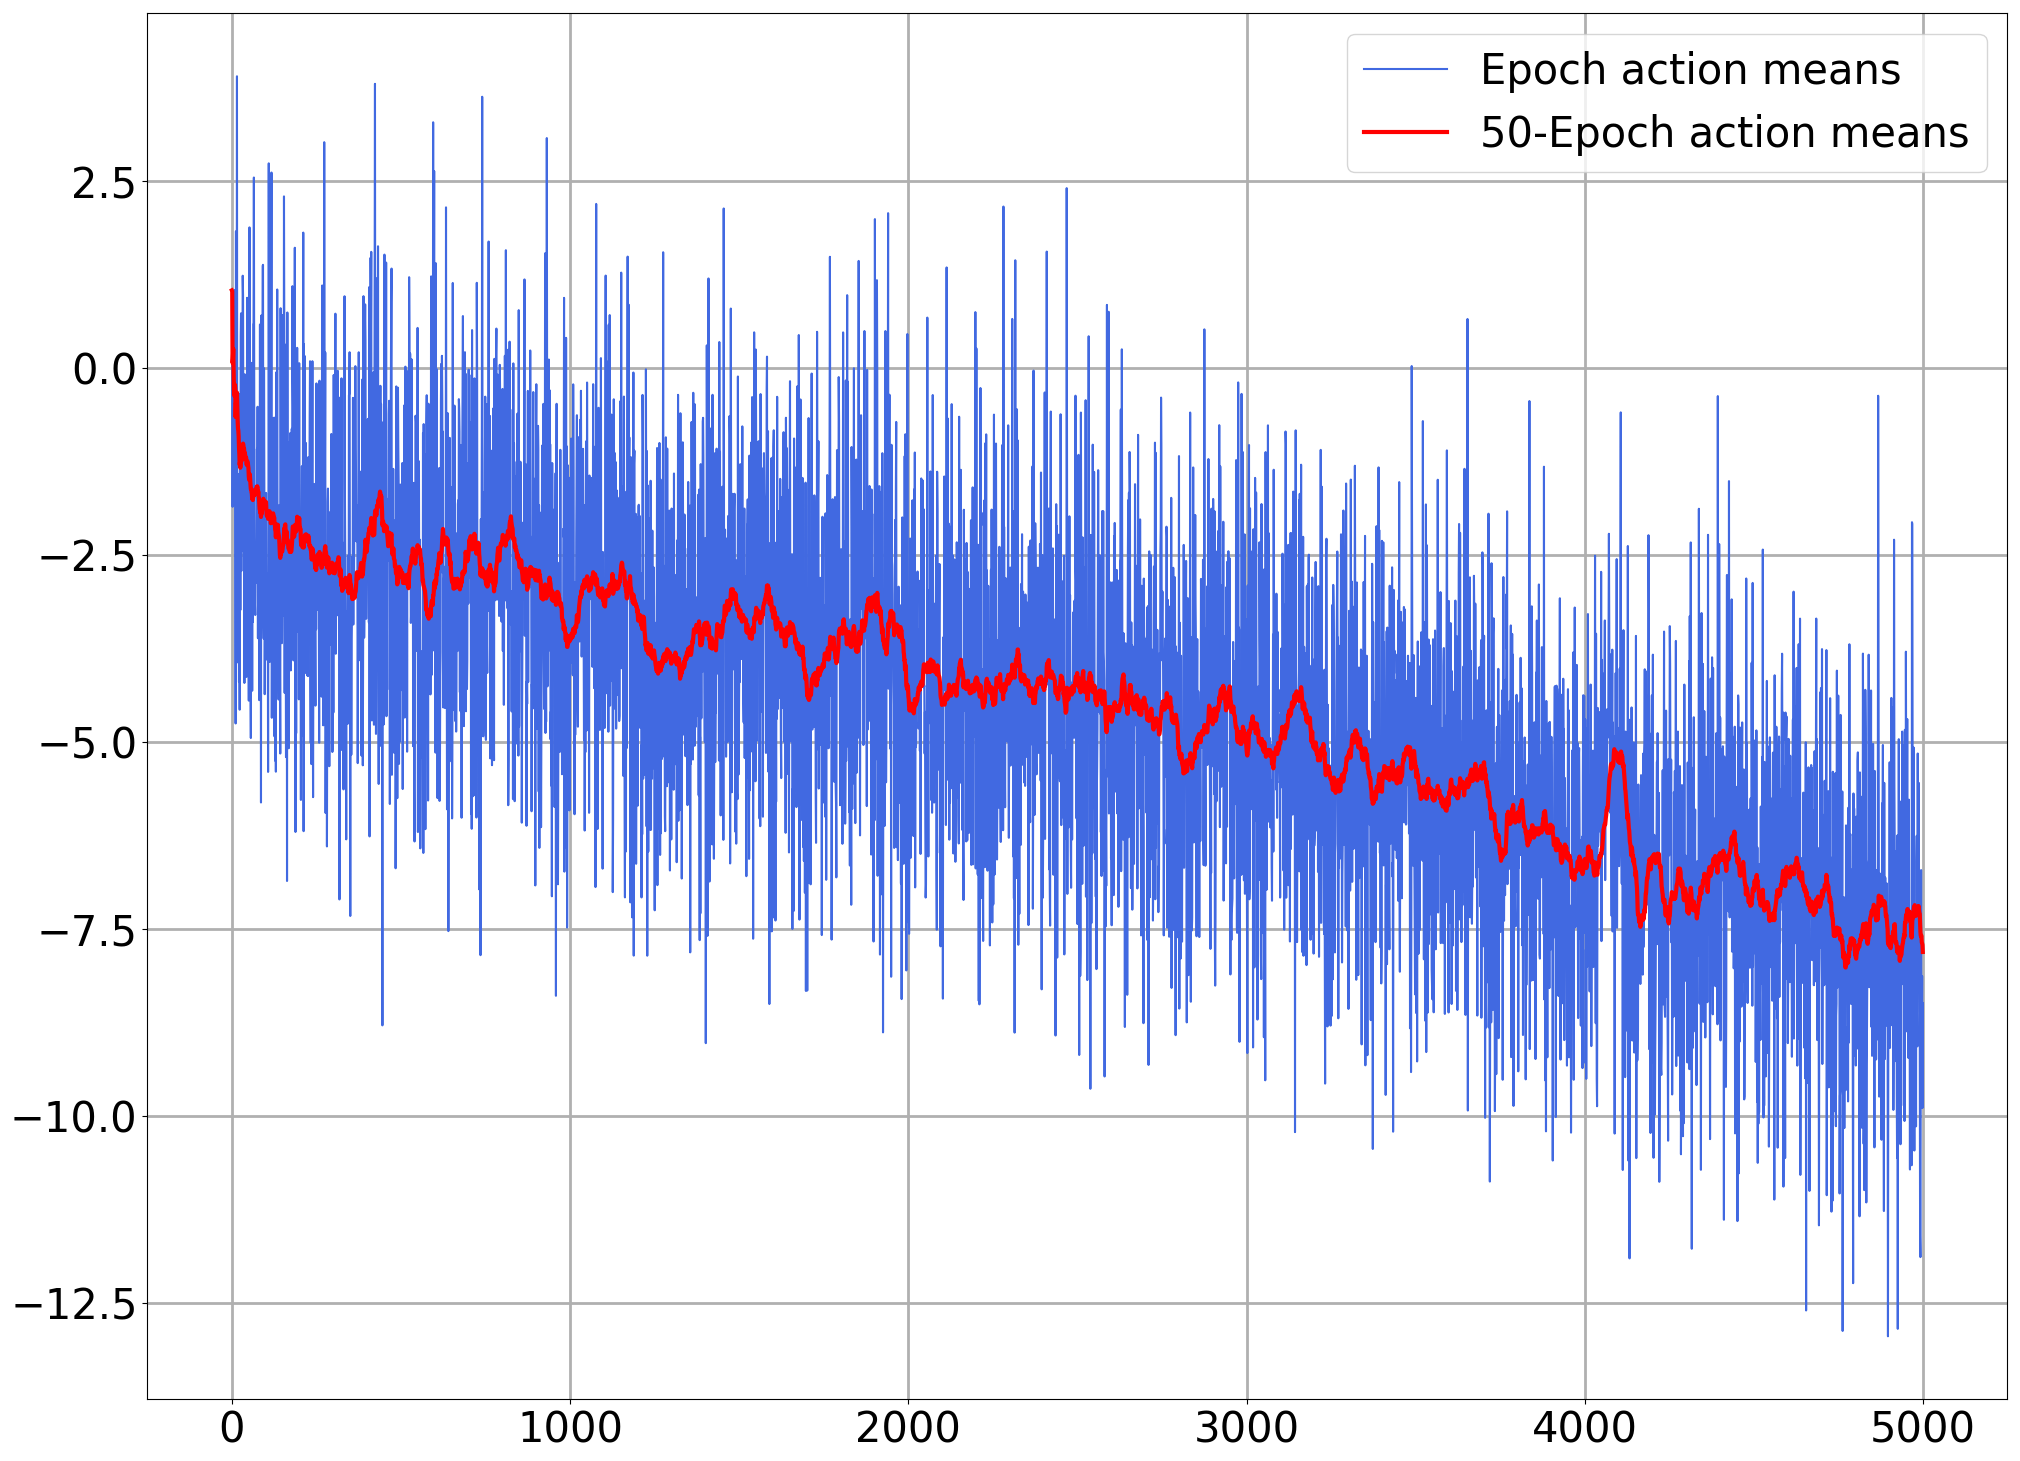
\includegraphics[width=\textwidth]{q_2_10000_BUY_mean_actions.png}
        \caption{Mean of actions per epoch (buy)}
        \label{fig:analysis-q-learn-2-action-buy}
    \end{subfigure}
    \begin{subfigure}[b]{0.4\textwidth}
        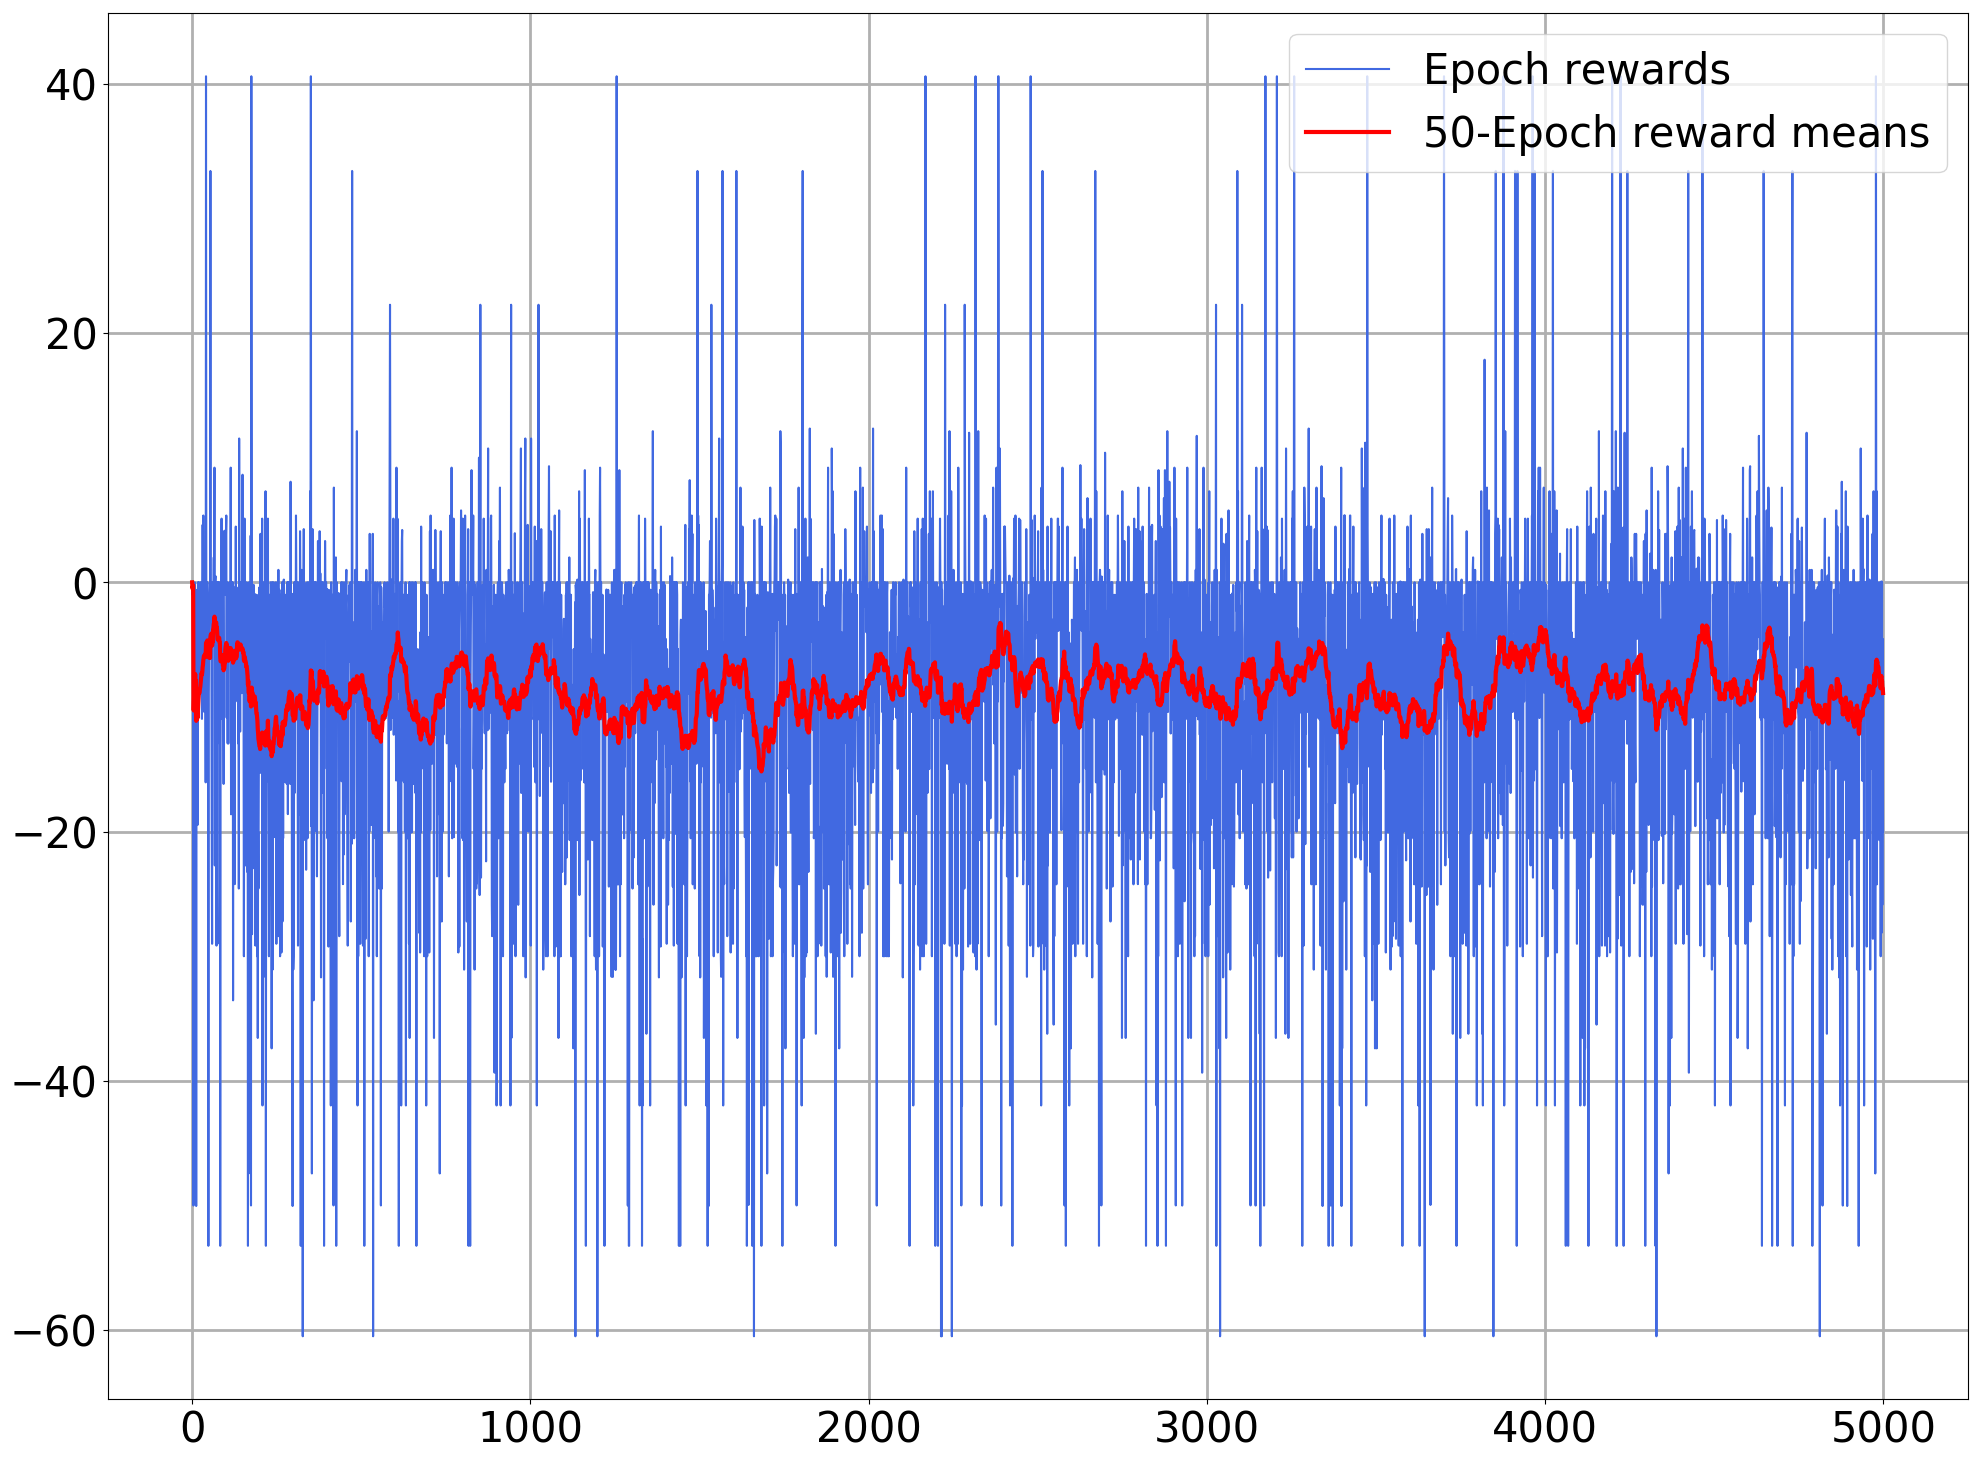
\includegraphics[width=\textwidth]{q_2_10000_SELL_rewards.png}
        \caption{Mean rewards per epoch (sell)}
        \label{fig:analysis-q-learn-2-reward-sell}
    \end{subfigure}
    \begin{subfigure}[b]{0.4\textwidth}
        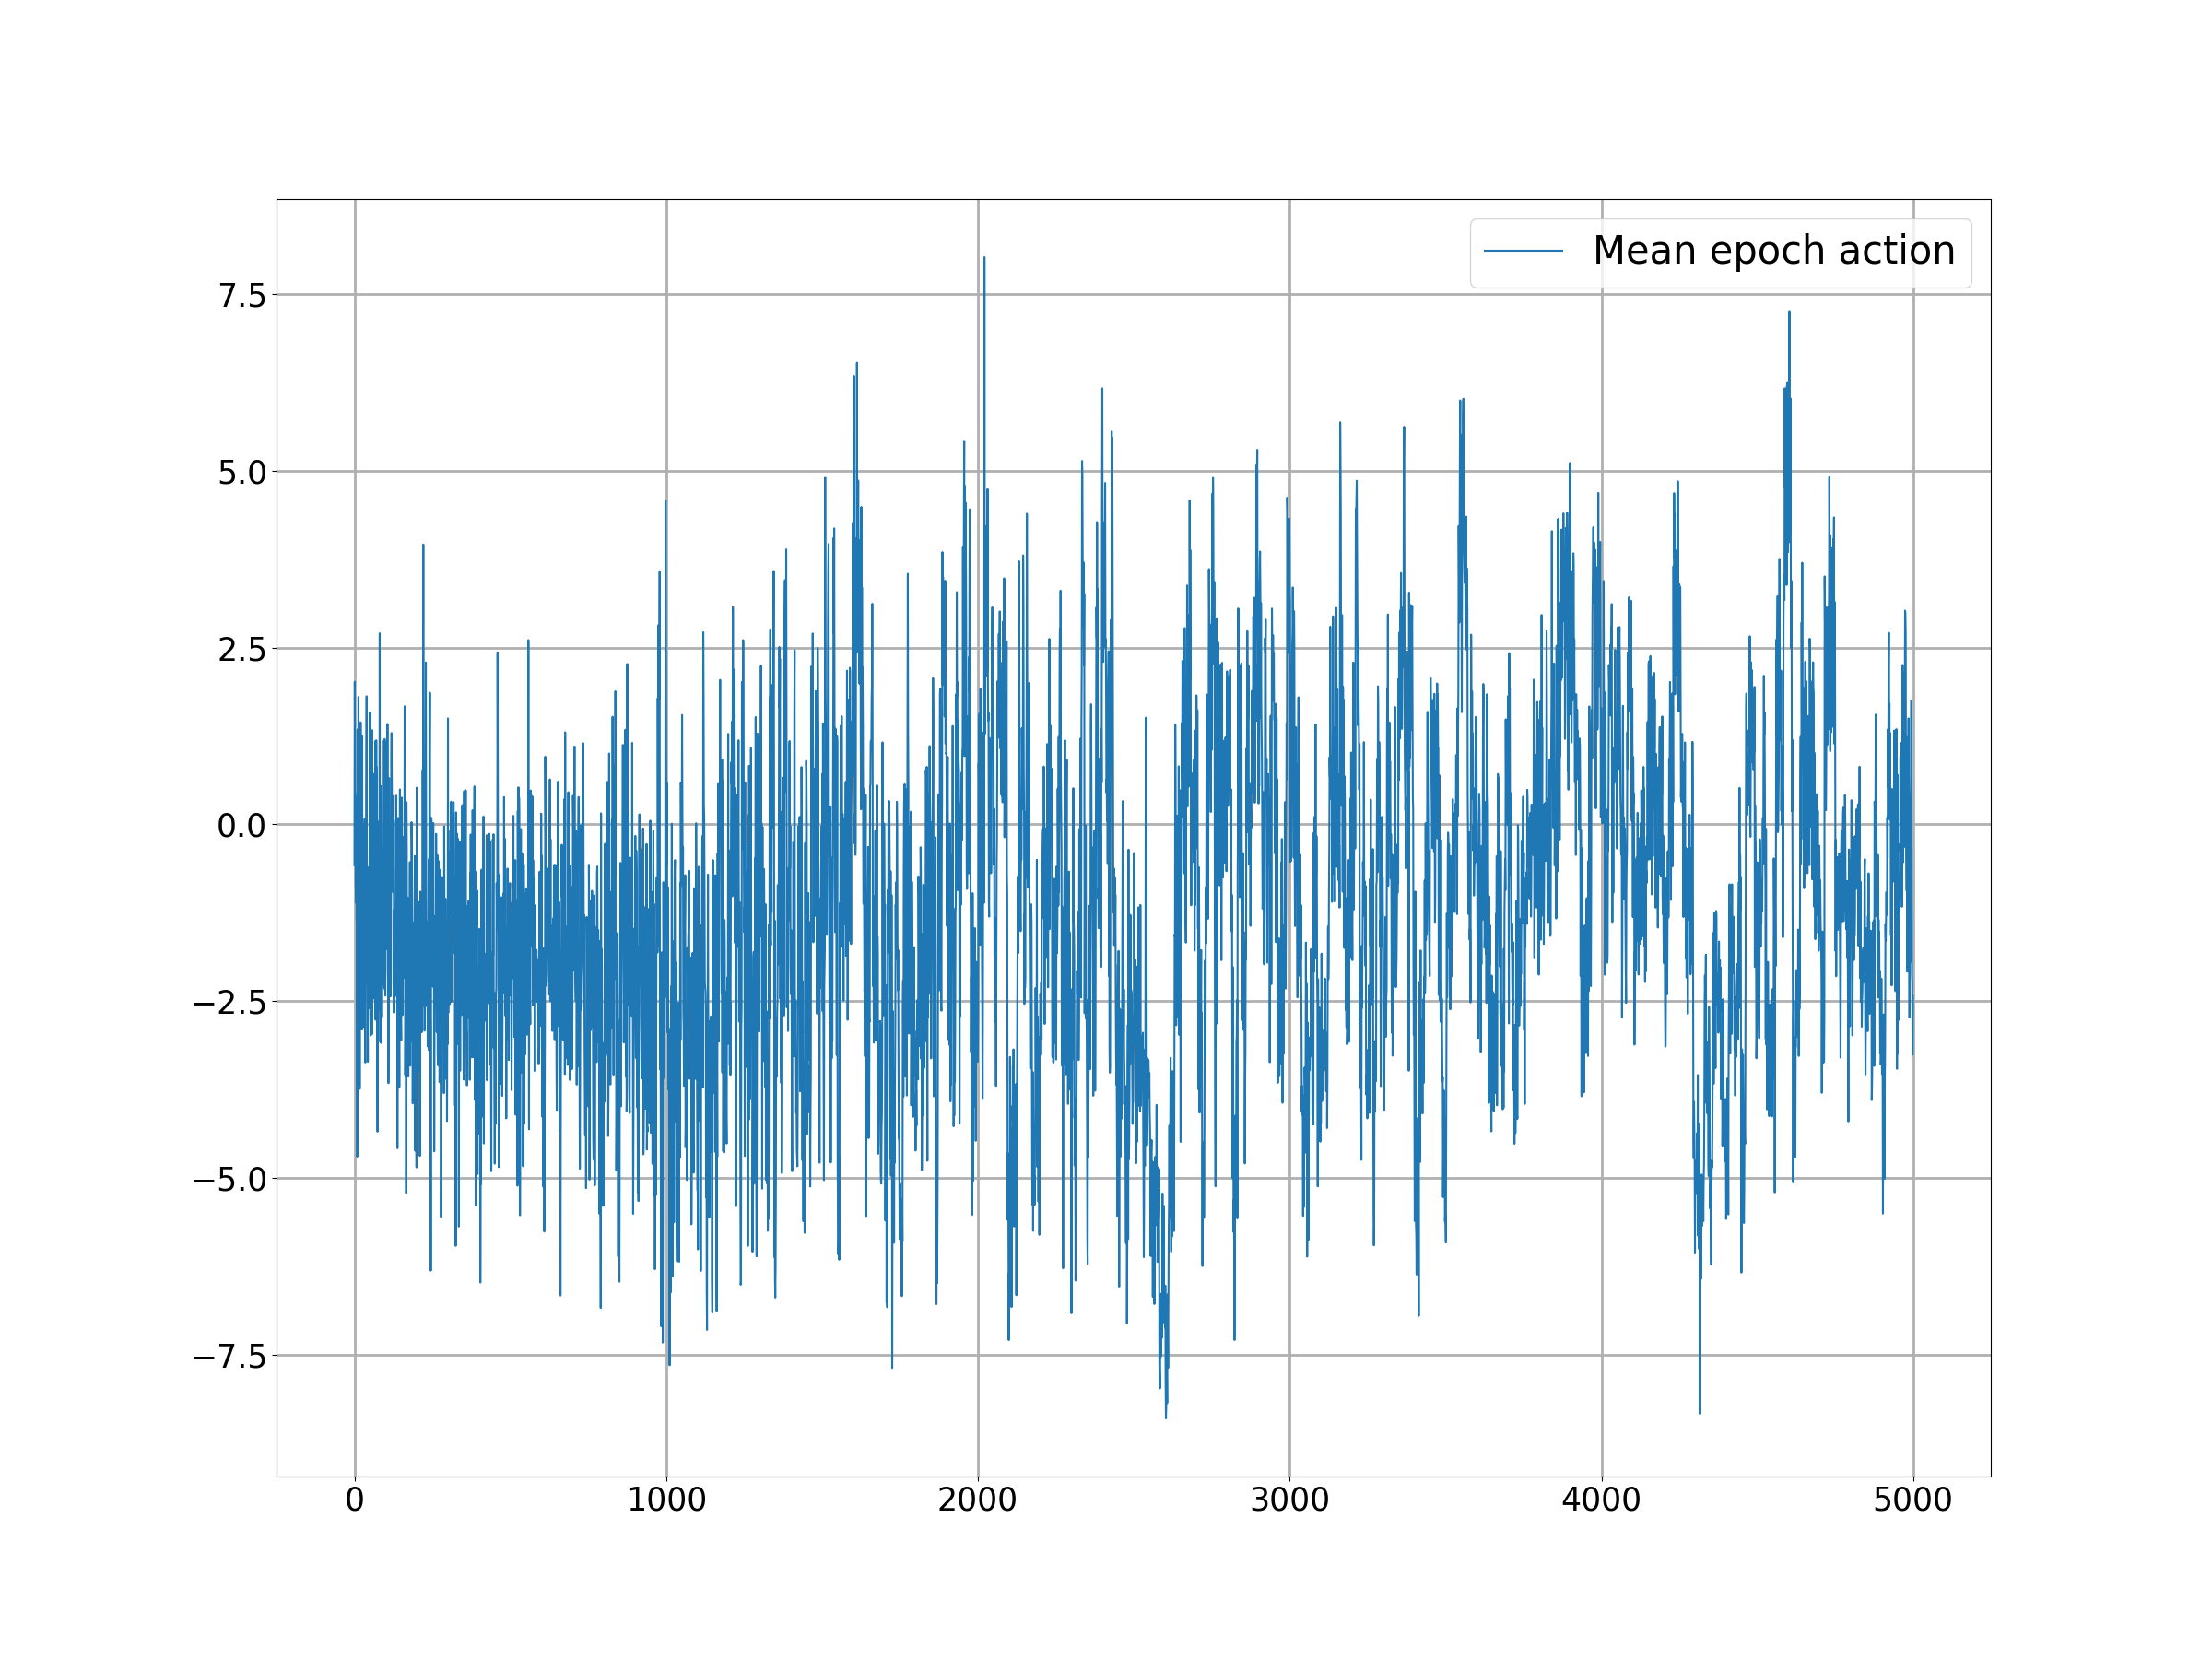
\includegraphics[width=\textwidth]{q_2_10000_SELL_mean_actions.png}
        \caption{Mean of actions per epoch (sell)}
        \label{fig:analysis-q-learn-2-action-sell}
    \end{subfigure}
    \caption{Mean rewards and actions for buying and selling on training data set II.}
    \label{fig:analysis-q-learn-2}
\end{figure}

Figure \ref{fig:analysis-q-learn-1} shows the training on data set I.
The average received reward during the training is shown in Figure \ref{fig:analysis-q-learn-1-reward-buy}.
Over the course of 5000 epochs, the agent was able to improve the mean reward by approximately $\sim$0.5, as a result of the change in actions chosen as illustrated in Figure \ref{fig:analysis-q-learn-1-action-buy}.
The agent started off with the average action of $\sim$-3 which is a result of the low epsilon parameter that makes the agent choose actions randomly.
Actions where then adapted to the more negative side of the order book, such that after $\sim$1500 epochs the agent choose actions as low as -20 and then adjusted and stagnated at $\sim$-15.
The backtest, during which 1000 orders were executed on the test data set, resulted in an average reward of \textit{-1.17}.
Comparing the results to the empirical analysis proceeded on the same data set, as shown in Figure \ref{fig:behvaiour-down}, provides means for interpretation:
The policy learned by the Q-Learning agent performs worse than the expected cost of a market order, which was \$-1.12 when buying 1.0 BTC and is shown in Section \ref{sec:eval-empirical}.
The highly negative average actions the agent choose towards the end of the training indicates that the order might have oftentimes not been able to be filled within the time horizon and an expensive market order had to follow.

The rewards received for the agents tasks to sell the assets are much more volatile than for buying, as shown in Figure \ref{fig:analysis-q-learn-1-reward-sell}, and no clear improvement can be seen.
In addition, there was no significant adjustment made by the agent regarding the mean of the actions chosen, as indicated in Figure \ref{fig:analysis-q-learn-1-action-sell}.
The backtest resulted in an average reward of -21.34 achieved by the agent.
The reward received for placing market orders on the test set account to a negative reward of -27.70.
Hence, the agent is able to save \$6.36 when selling 1.0 BTC.
\\
\\
Figure \ref{fig:analysis-q-learn-2} shows the experiment proceeded on data set II.
The average reward received while training to buy the asset is shown in Figure \ref{fig:analysis-q-learn-2-reward-buy}.
Throughout the epochs, the agent was able to improve the mean reward similar as with the previous data set I, by approximately 0.5.
Even though the trend of this data set is the opposite, the change in chosen actions correlates to the previous findings and is illustrated in Figure \ref{fig:analysis-q-learn-2-action-buy}.
The backtest on the test data set II, resulted in an average reward of \textit{-1.04} -- again worse than the average reward received on the training set.
A market order on this test data accounts to an average reward of -1.06, indicating that the agents policy is saving \$0.02 when buying 1.0 BTC.
Considering the empirical analysis proceeded for buying on this data set, as shown in Figure \ref{fig:behvaiour-up}, and comparing it to the received rewards by the agent, implies that the agent failed to execute orders with the placed limit orders and oftentimes market orders must have followed.

Similar to the sell orders placed on data set I, the rewards received for the agents tasks to sell the assets on data set II are very volatile, as shown in Figure \ref{fig:analysis-q-learn-1-reward-sell}.
No improvement can be seen from the rewards during the training and no significant adjustment was made by the agent regarding the chosen actions, as indicated in Figure \ref{fig:analysis-q-learn-2-action-sell}.
The backtest resulted in an average reward of -4.74 achieved by the agent, whereas market orders are expected to result in an average reward of -1.72.
Hence, the agent causes to pay a premium of \$3.02 for selling 1.0 BTC.

\subsection{Conclusion of Q-Learning approach}

\begin{table}[H]
\centering
\begin{tabular}{l|l|l|}
\cline{2-3}
& \textbf{Q-Learner} & \textbf{\begin{tabular}[c]{@{}l@{}}$\mathbb{E}$[Market\\ Order]\end{tabular}} \\ \hline
\multicolumn{1}{|l|}{\textbf{Buy (I)}}   & -1.17          & -0.05                                                           \\ \hline
\multicolumn{1}{|l|}{\textbf{Sell (I)}}  & -21.34         & -27.70                                                          \\ \hline
\multicolumn{1}{|l|}{\textbf{Buy (II)}}  & -1.04          & -1.06                                                           \\ \hline
\multicolumn{1}{|l|}{\textbf{Sell (II)}} & -4.74          & -1.72                                                           \\ \hline
\end{tabular}
\caption{Summary of rewards for the Q-Learning agent and market orders.}
\label{tbl:analysis-q-learn-summary}
\end{table}
The findings of this section are summarized in Table \ref{tbl:analysis-q-learn-summary}.
We conclude that the Q-Learning agent was not able to constantly place buy and sell orders in a way which would result in a price better than the current market price.
Oftentimes, a market order, which would cause an immediate purchase or sale, would be the better choice.
Clearly, this is due to the fact that the agent was not able to find the most suitable actions.
Furthermore, in order to investigate whether or not these findings were a result of the agent aiming for too much immediate reward, the same experiment was proceeded with $\gamma=0.3$ and therefore rely more extensively on the future rewards.
However, no improvement could be achieved and instead the agent achieved similar rewards while requiring more epochs in order to converge to the same mean of actions.
In this section we have only investigated the mean of the actions chosen throughout an epoch, which gave enough proofs that the chosen actions resulted mostly in market orders.
Furthermore, it is to be assumed that the absence of market variables, while only relying on the given rewards, makes it hard for any learner to determine an optimal policy.
Therefore, the following section will make use of market variables in order to determine whether or not a learner can exploit the information hidden in the market and therefore act in favor of optimally placing limit orders.

\section{Deep Q-Network with market features}
\label{sec:eval-dqn}
In the previous section, the Q-Learning agent was trained on data sets I and II, and no significant optimization in terms of buying and selling assets was achieved.
By considering the previously found results of the empirical analysis of the limit order placement behaviour we found that most of the limit orders placed by the Q-Learning agent were not filled within the given time horizon and instead market orders had to be submitted after the time was consumed.

In this section we aim to determine whether or not the DQN agent is capable of extracting information provided by the raw market features and therefore improve the limit order placement policy.
The setup is the same as in the previous section where the agents task is to buy and sell 1.0 BTC within 100 seconds with discrete step size $\Delta{t}=10$ on both data sets I and II.
Furthermore, both features, which were constructed in Chapter \ref{chap:data}, will be applied and investigated separately.
The input shape of the model in use that approximates the action-value function, as described in Chapter \ref{chap:preliminaries} (Section \ref{sec:deep-reinforcement-learning}), is therefore determined by the chosen feature and is described below.
After extensive investigations with multiple such models, including various multi-layer neural networks\cite{svozil1997introduction} and a long short-term neural network (LSTM)\cite{gers1999learning} and a convolutional neural network (CNN), the best performance was achieved with the latter.
As a result, the model is use for this analysis is the CNN, as described in Chapter \ref{chap:setup} (Section \ref{setup:dqn}).
Therefore, for both DQN agents, we relied on the default hyperparameters worked out by Mnih et al. \cite{mnih2015human}, as shown in Figure \ref{fig:eval-dqn-hyperparameters}.
Finally, we conclude our findings and determine the capabilities of the DQN approach (and its use of the market features) by comparing it to the expected rewards found in Section \ref{sec:eval-empirical}.
\begin{figure}[H]
    \centering
    \makebox[\linewidth]{
        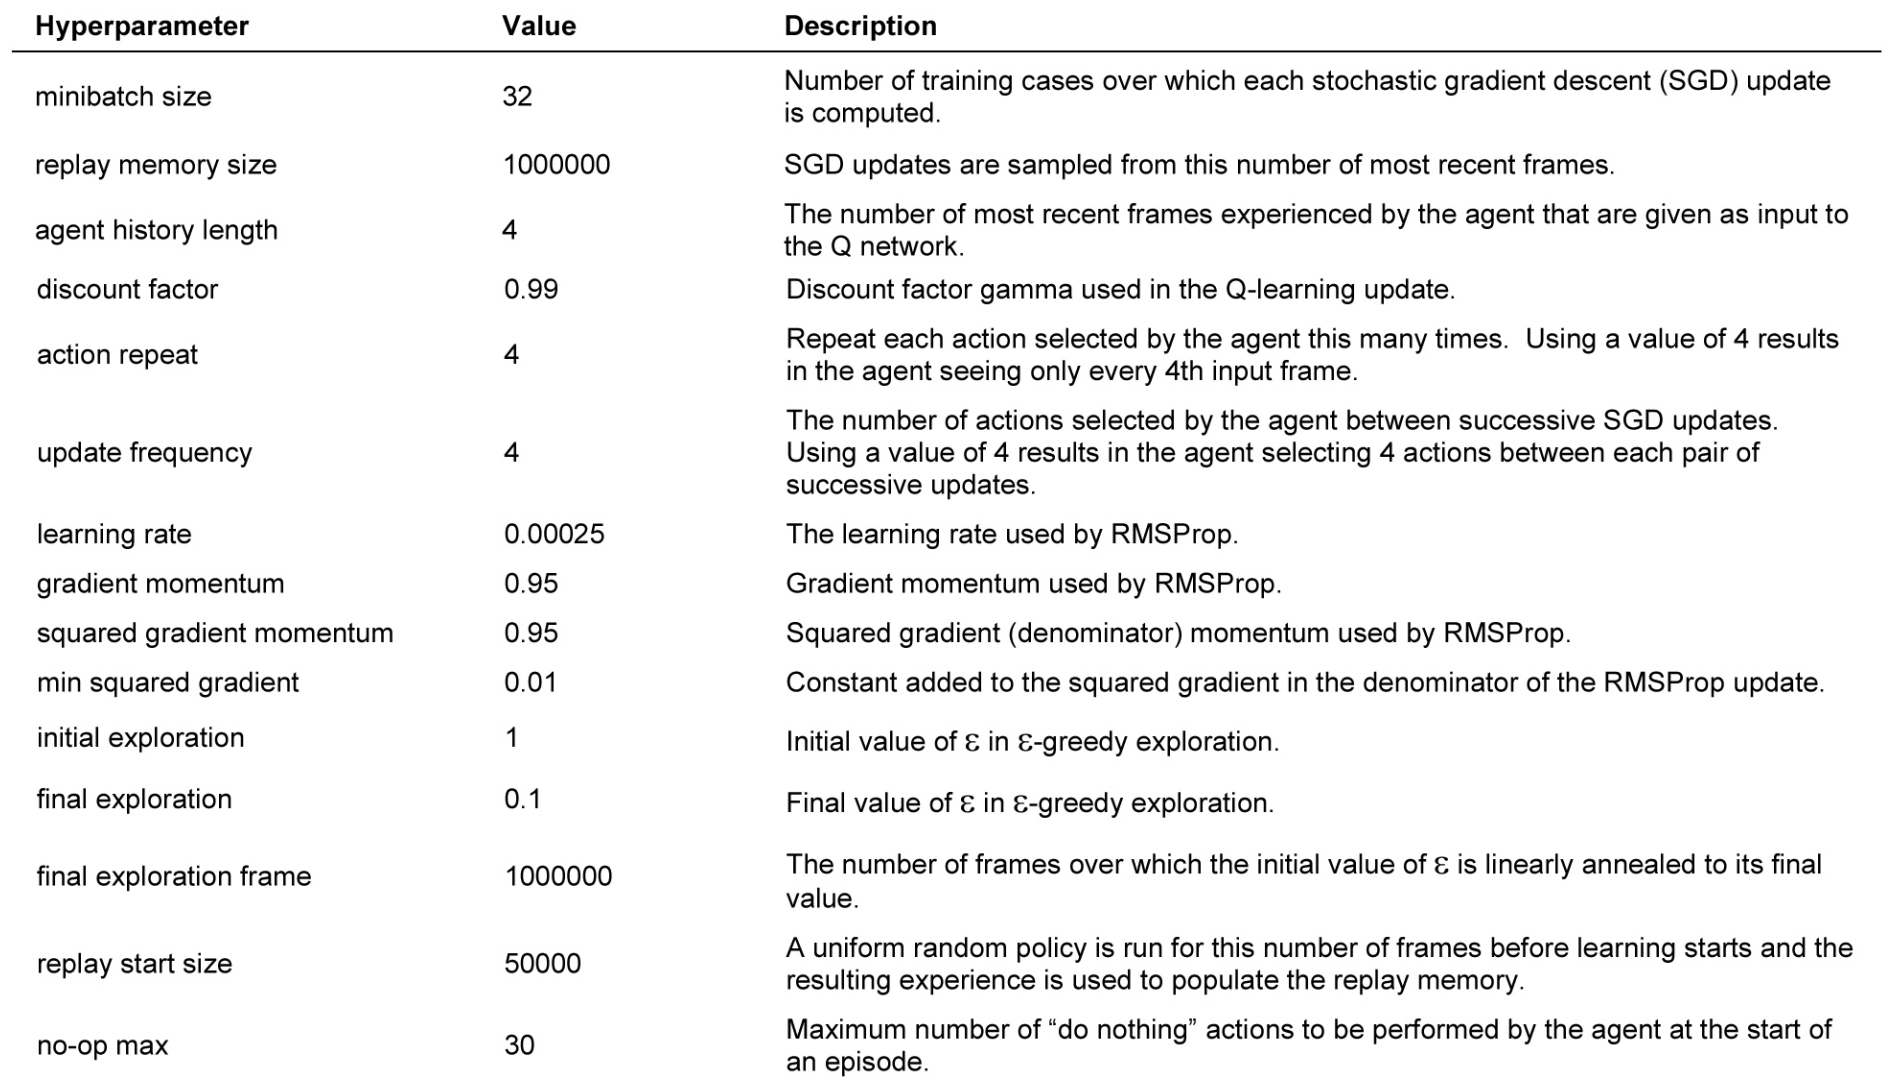
\includegraphics[width=14cm]{images/dqn_hyperparameters.png}
    }
    \caption{The values of all the hyperparameters were selected. We did not perform a systematic grid search owing to the high computational cost, although it is conceivable that better results could be obtained by tuning these hyperparameter values.}
    \label{fig:eval-dqn-hyperparameters}
\end{figure}

\subsection{Application of historical order feature}

The following evaluation of the DQN agent considers historical order book states as described in Chapter \ref{chap:data} (Section \ref{sec:data-feature-1}) which we denote henceforth as Feature I.
Therefore, a \textit{lookback} of 30 historical order book states are considered and the number of level in each state is limited to 20 for bids and asks respectively.
Consequently this feature set is of size: $(2*lookback, limit levels, 2) \implies (60, 20, 2)$.
Including the two private variables by appending a vector $[inventory, time]$ at the beginning of this feature vector results a feature set size of: $(61, 20, 2)$ and serves as the input for the CNN.

\begin{figure}[H]
    \centering
    \begin{subfigure}[b]{0.4\textwidth}
        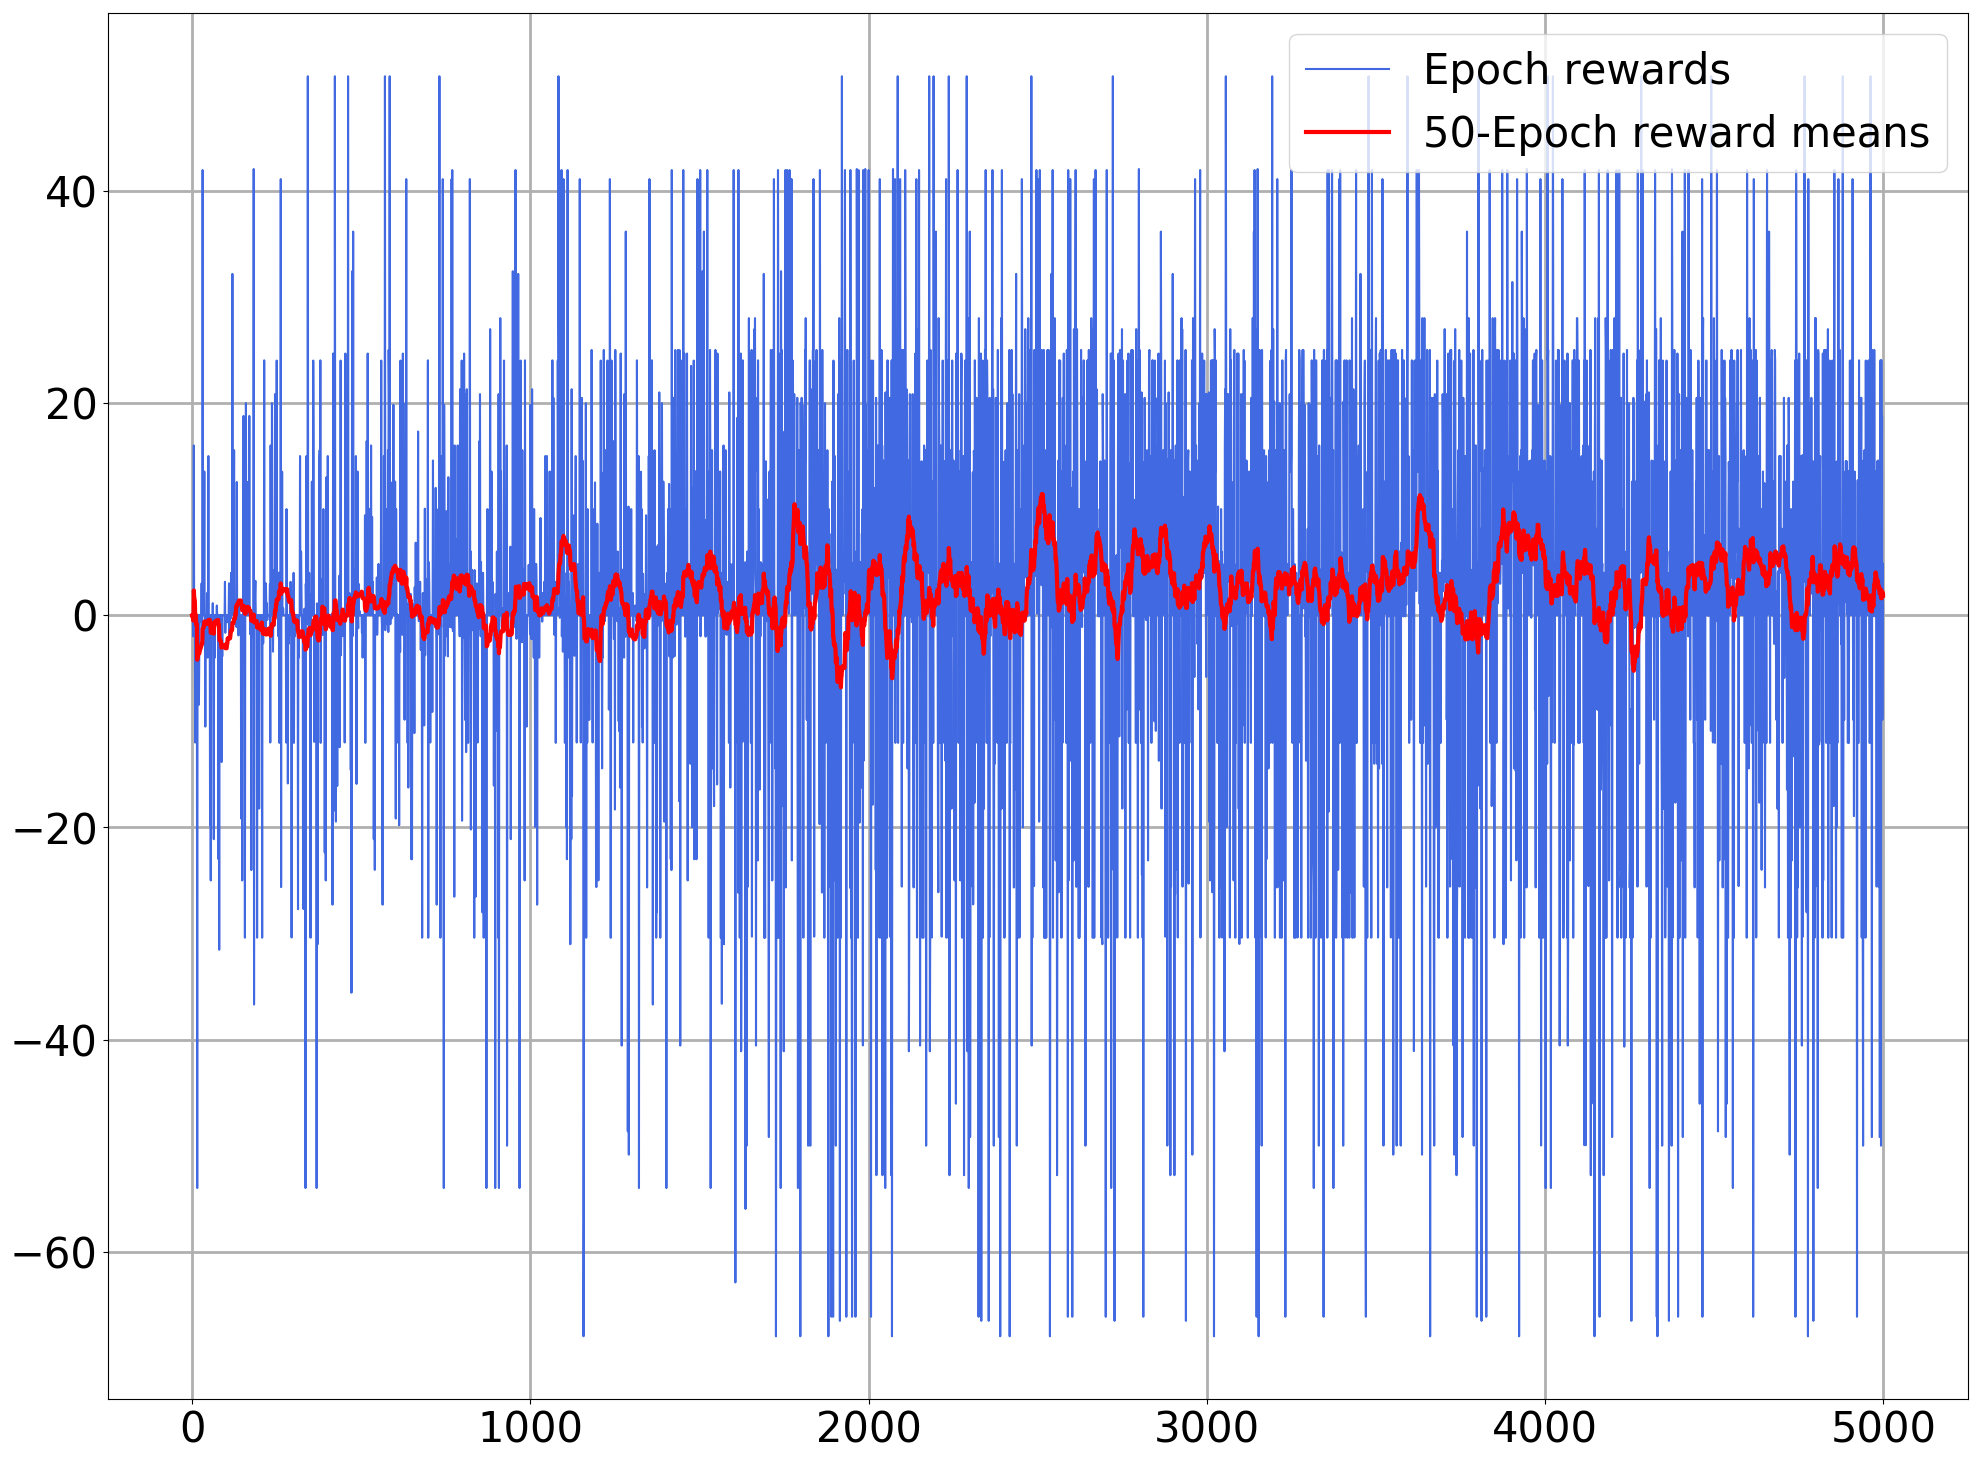
\includegraphics[width=\textwidth]{cnn_1_buy_rewards.png}
        \caption{Reward per epoch (buy)}
        \label{fig:analysis-dqn-1-reward-buy}
    \end{subfigure}
    \begin{subfigure}[b]{0.4\textwidth}
        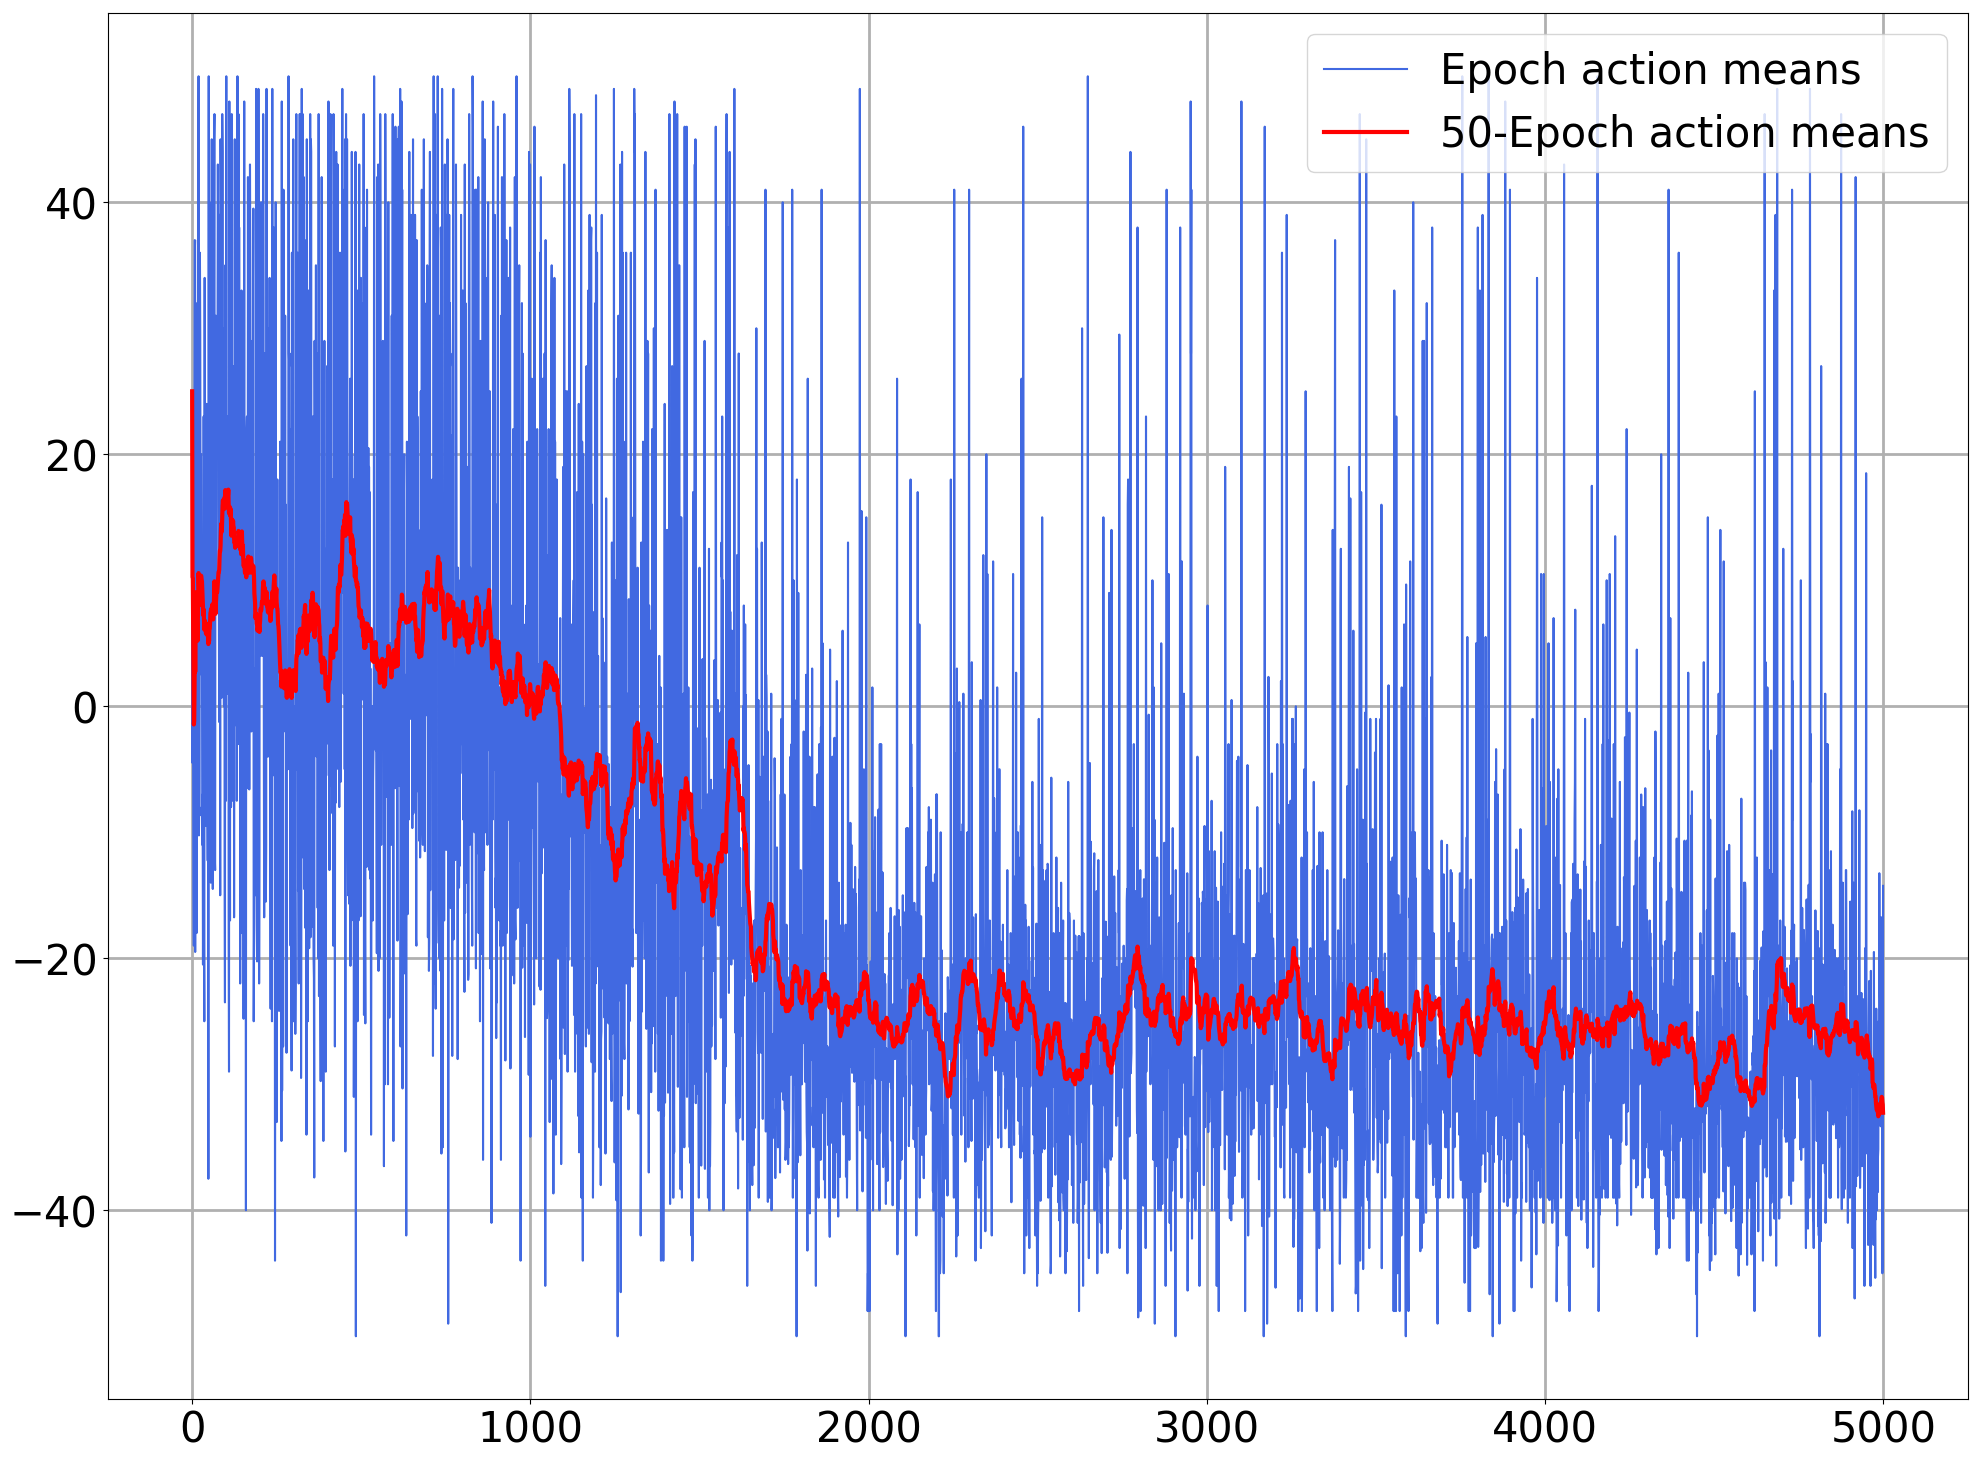
\includegraphics[width=\textwidth]{cnn_1_buy_mean_actions.png}
        \caption{Mean of actions per epoch (buy)}
        \label{fig:analysis-dqn-1-action-buy}
    \end{subfigure}
    \begin{subfigure}[b]{0.4\textwidth}
        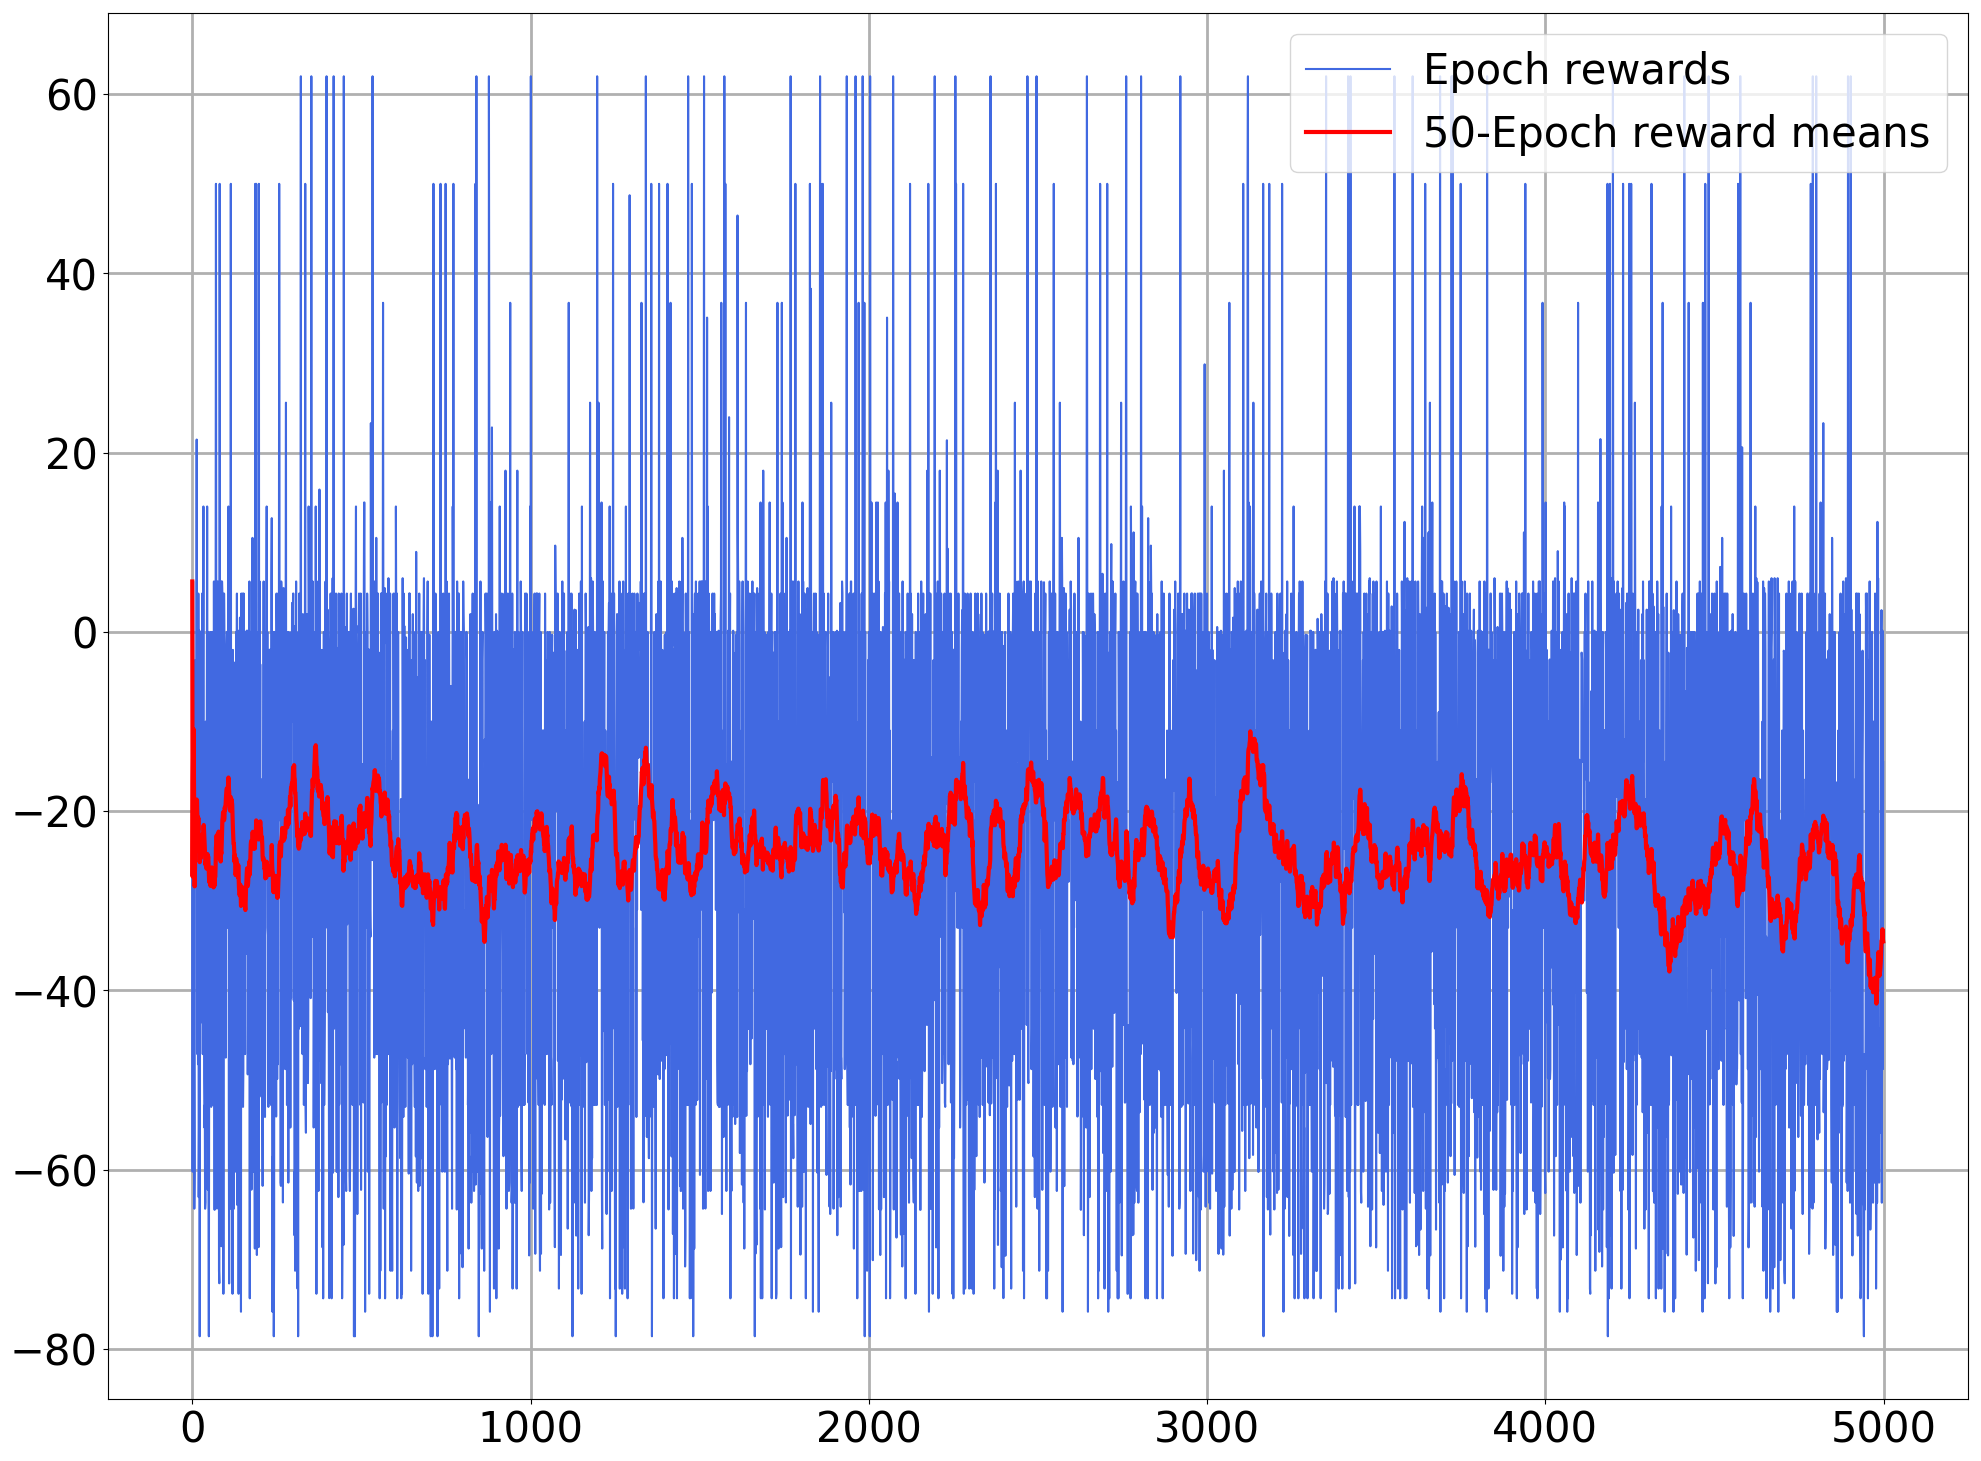
\includegraphics[width=\textwidth]{cnn_1_sell_rewards.png}
        \caption{Mean rewards per epoch (sell)}
        \label{fig:analysis-dqn-1-reward-sell}
    \end{subfigure}
    \begin{subfigure}[b]{0.4\textwidth}
        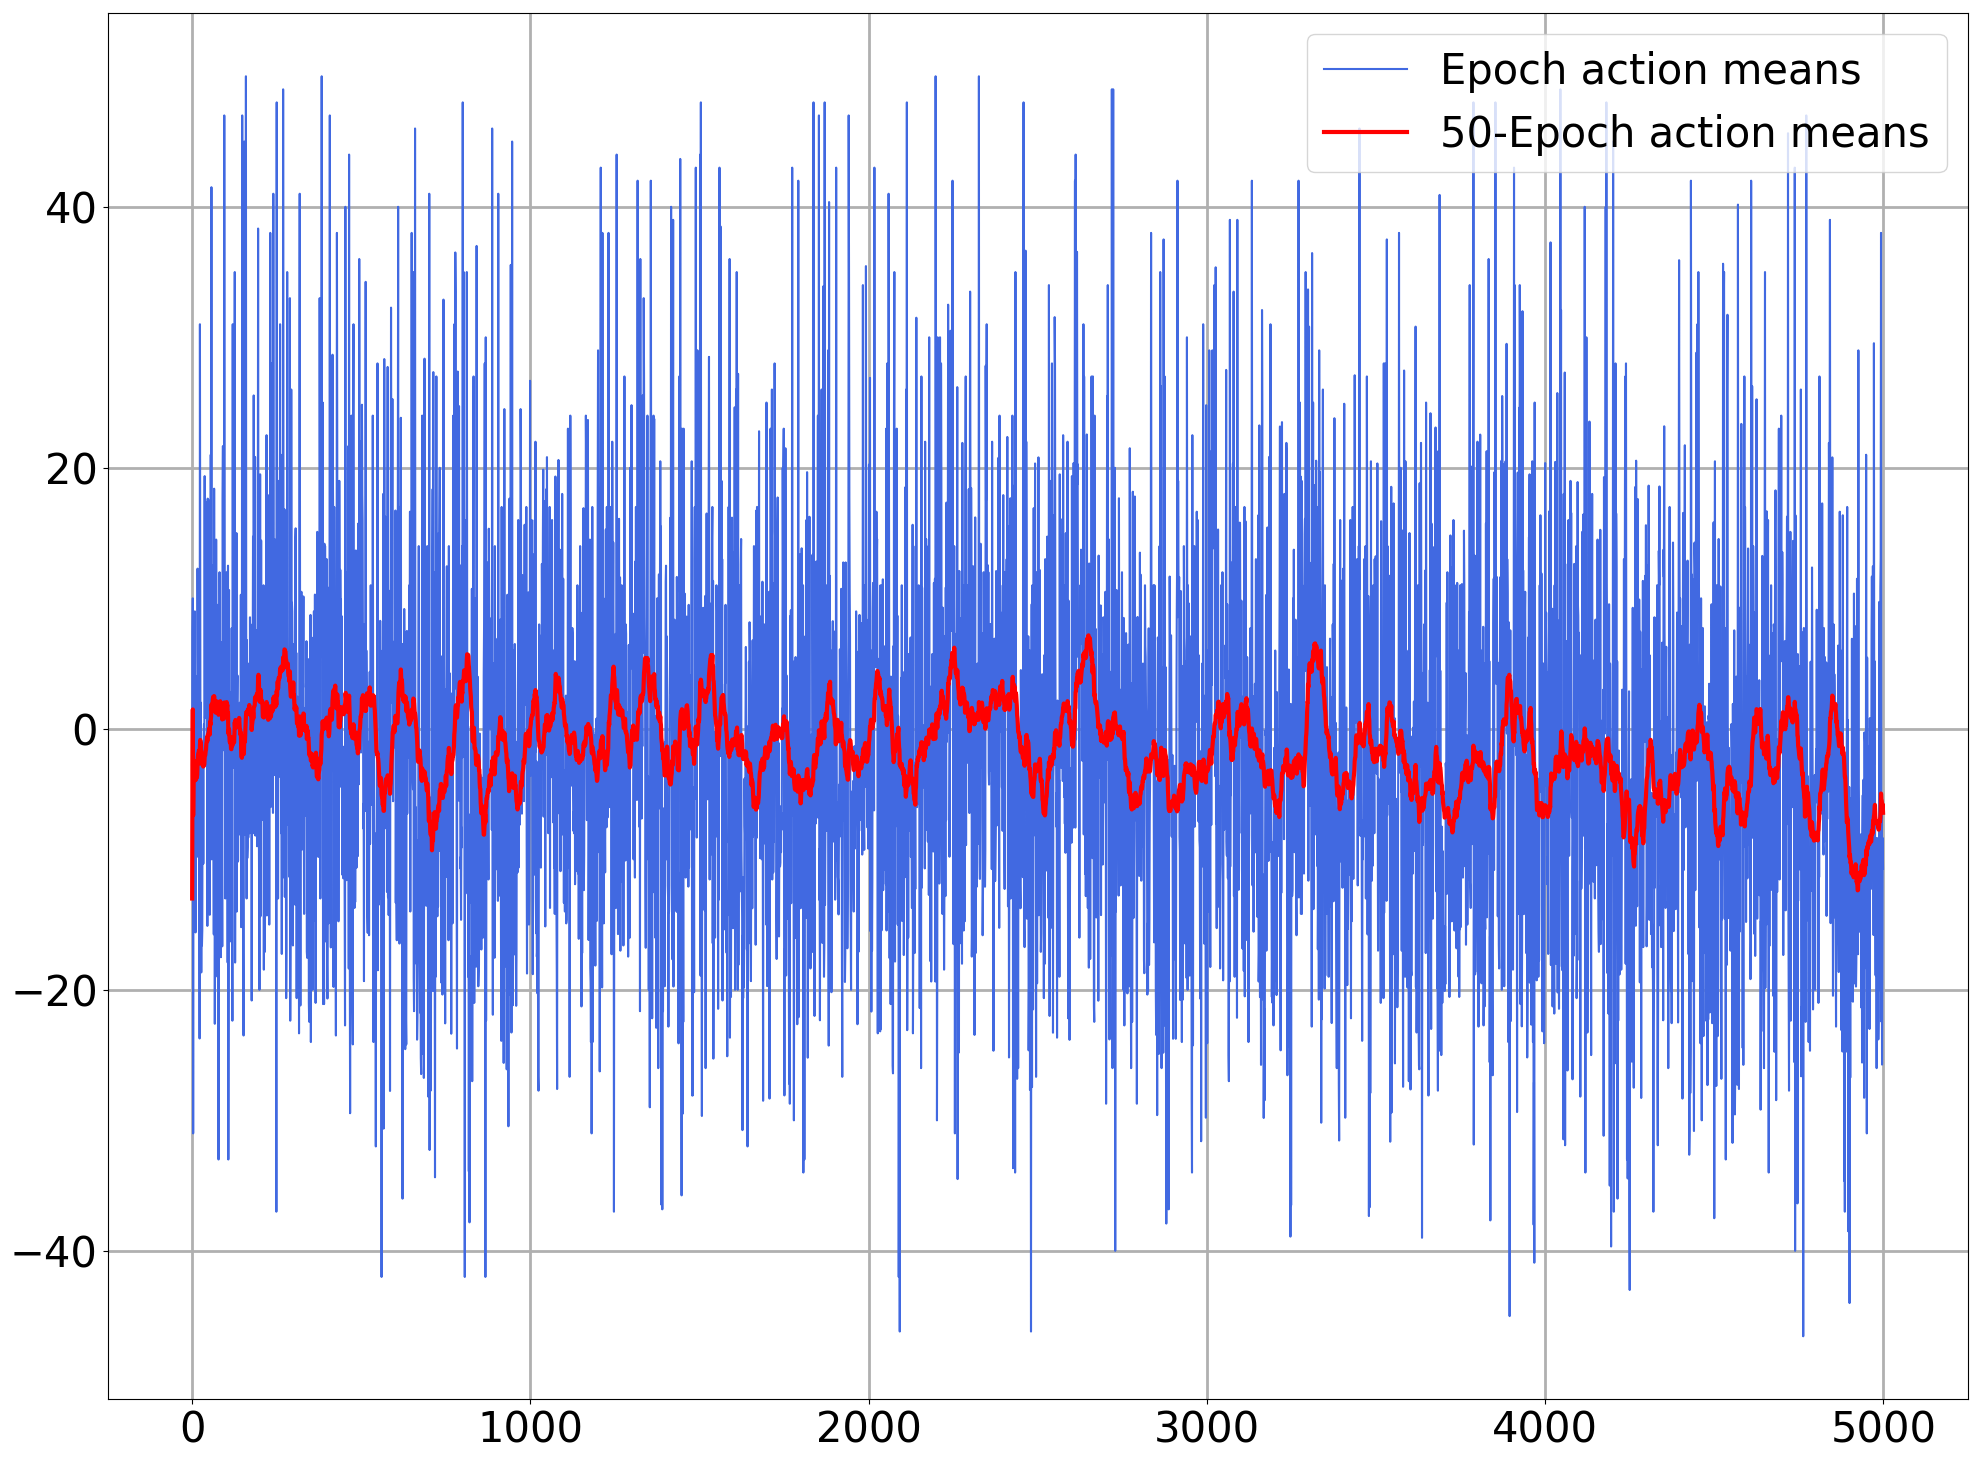
\includegraphics[width=\textwidth]{cnn_1_sell_mean_actions.png}
        \caption{Mean of actions per epoch (sell)}
        \label{fig:analysis-dqn-1-action-sell}
    \end{subfigure}
    \caption{DQN agent rewards and mean of actions for buying and selling on training data set I using feature I.}
    \label{fig:analysis-dqn-1}
\end{figure}

\begin{figure}[H]
    \centering
    \begin{subfigure}[b]{0.4\textwidth}
        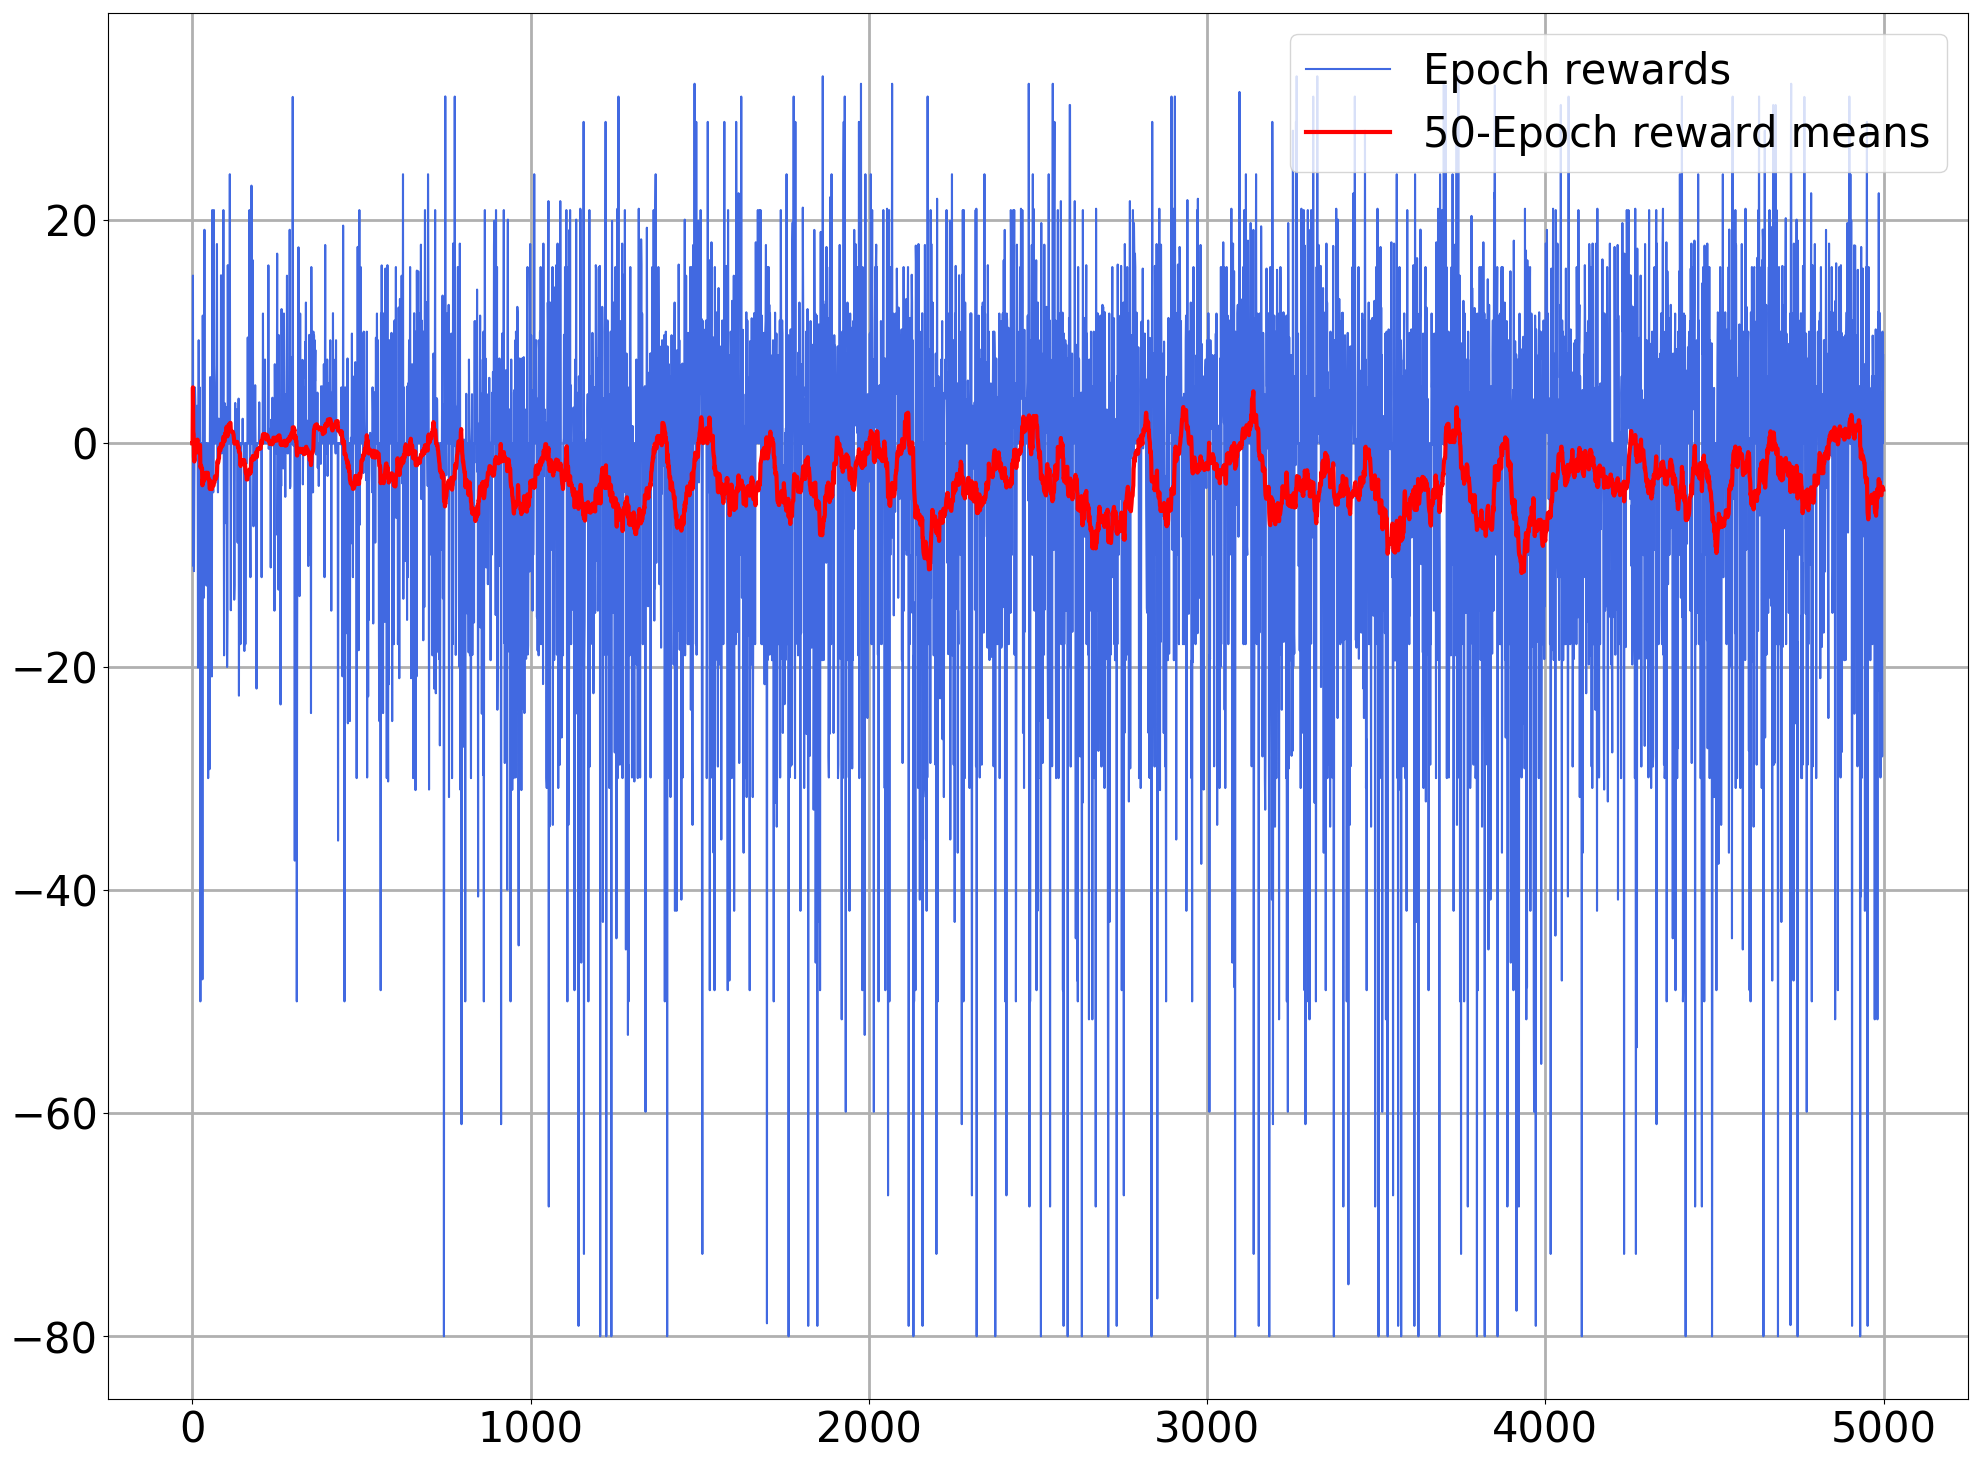
\includegraphics[width=\textwidth]{cnn_2_buy_rewards.png}
        \caption{Reward per epoch (buy)}
        \label{fig:analysis-dqn-2-reward-buy}
    \end{subfigure}
    \begin{subfigure}[b]{0.4\textwidth}
        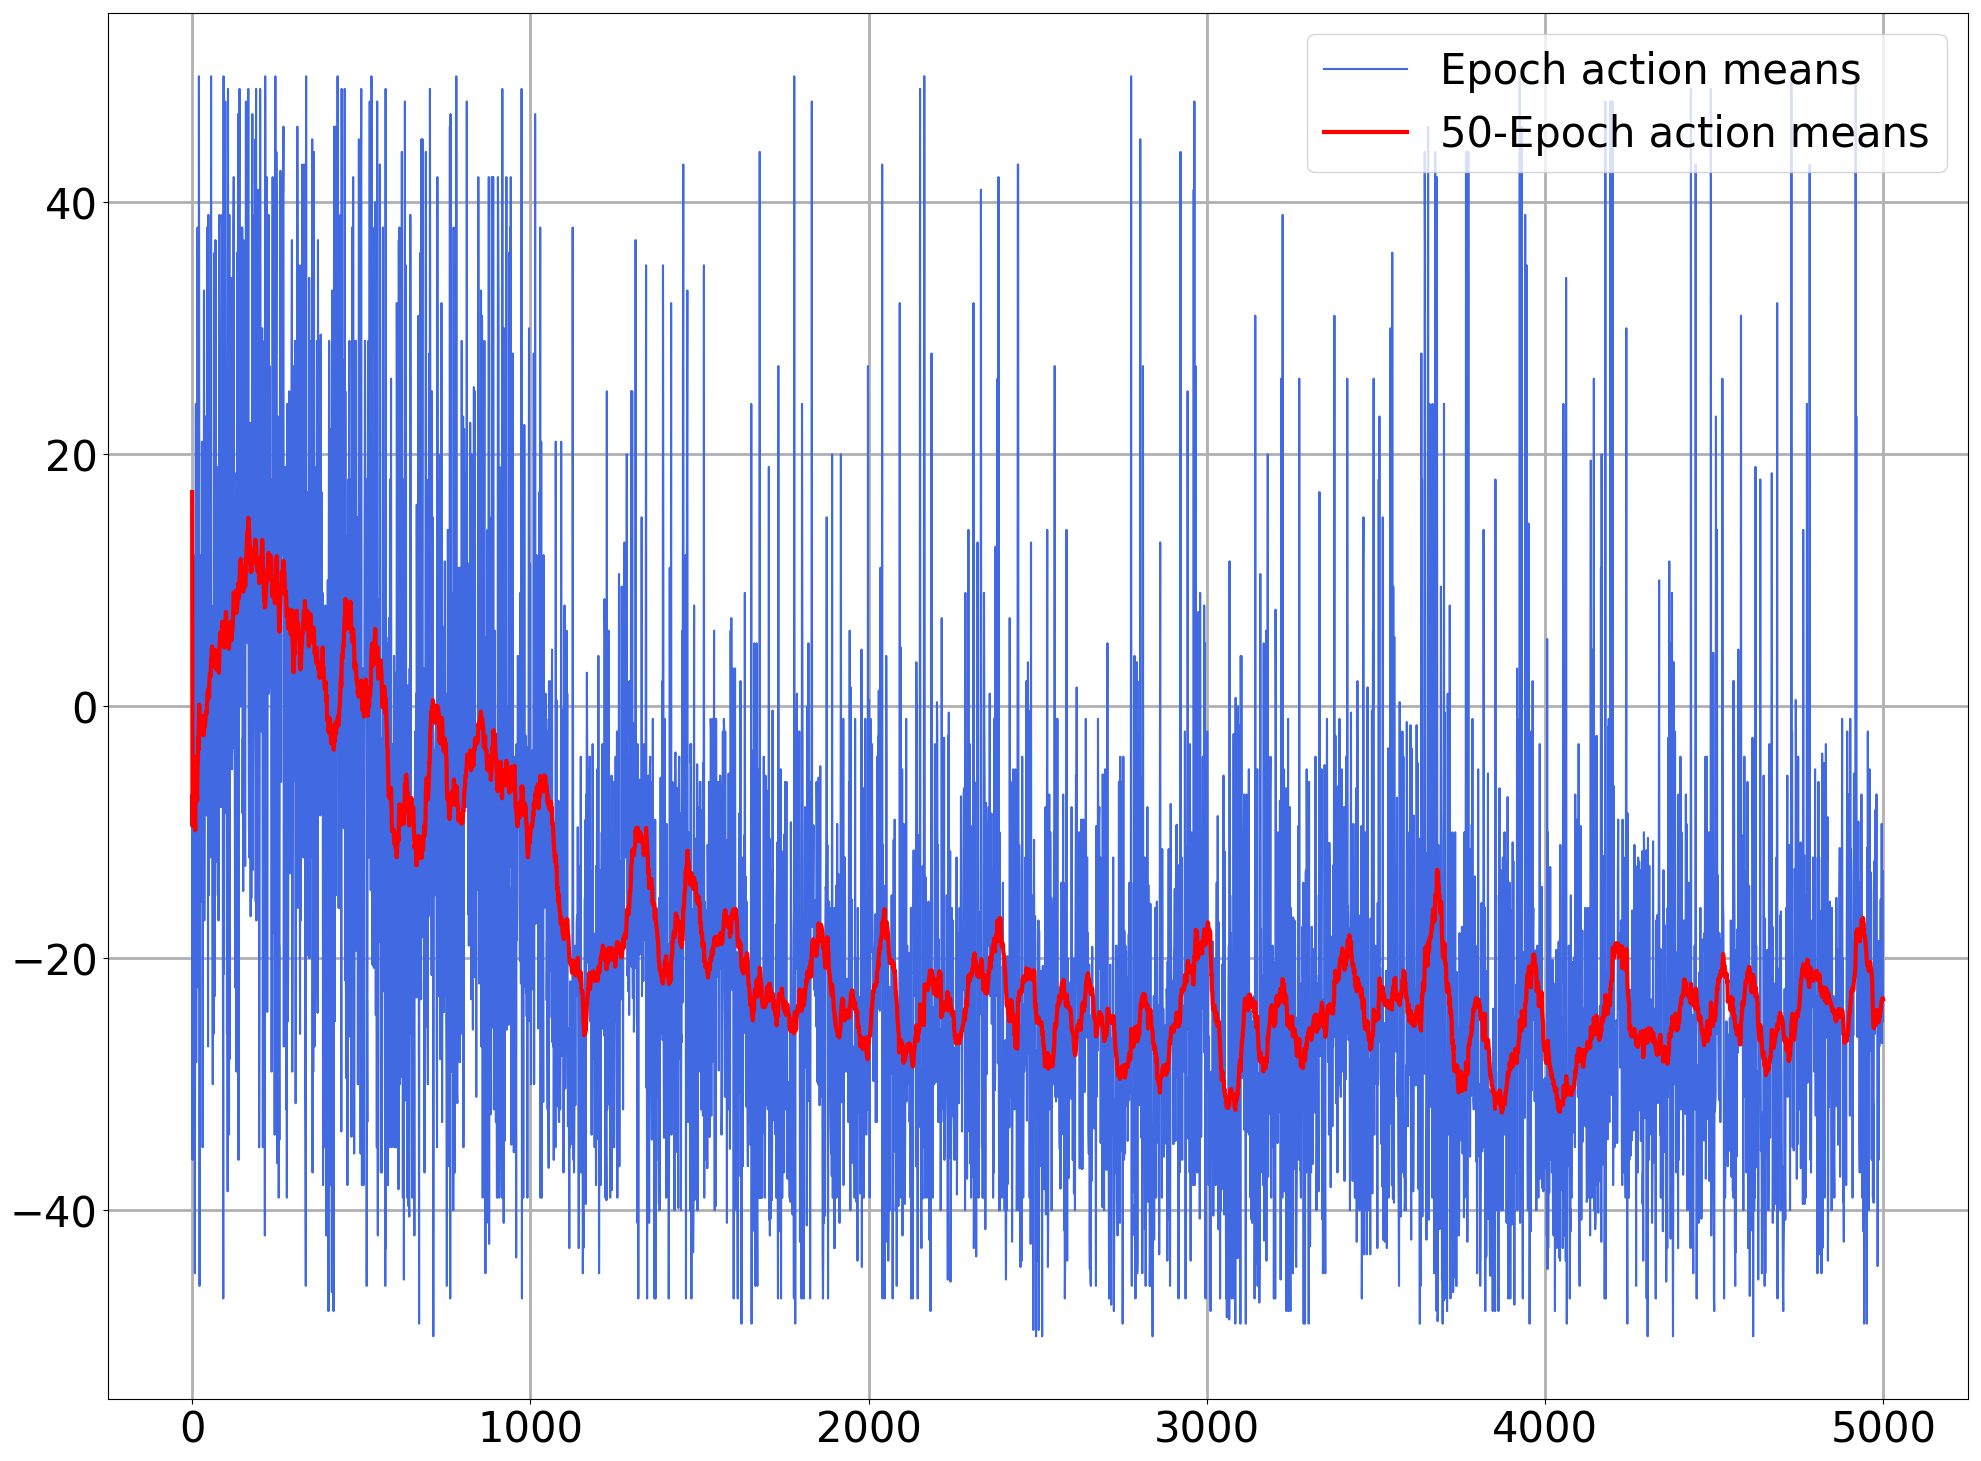
\includegraphics[width=\textwidth]{cnn_2_buy_mean_actions.png}
        \caption{Mean of actions per epoch (buy)}
        \label{fig:analysis-dqn-2-action-buy}
    \end{subfigure}
    \begin{subfigure}[b]{0.4\textwidth}
        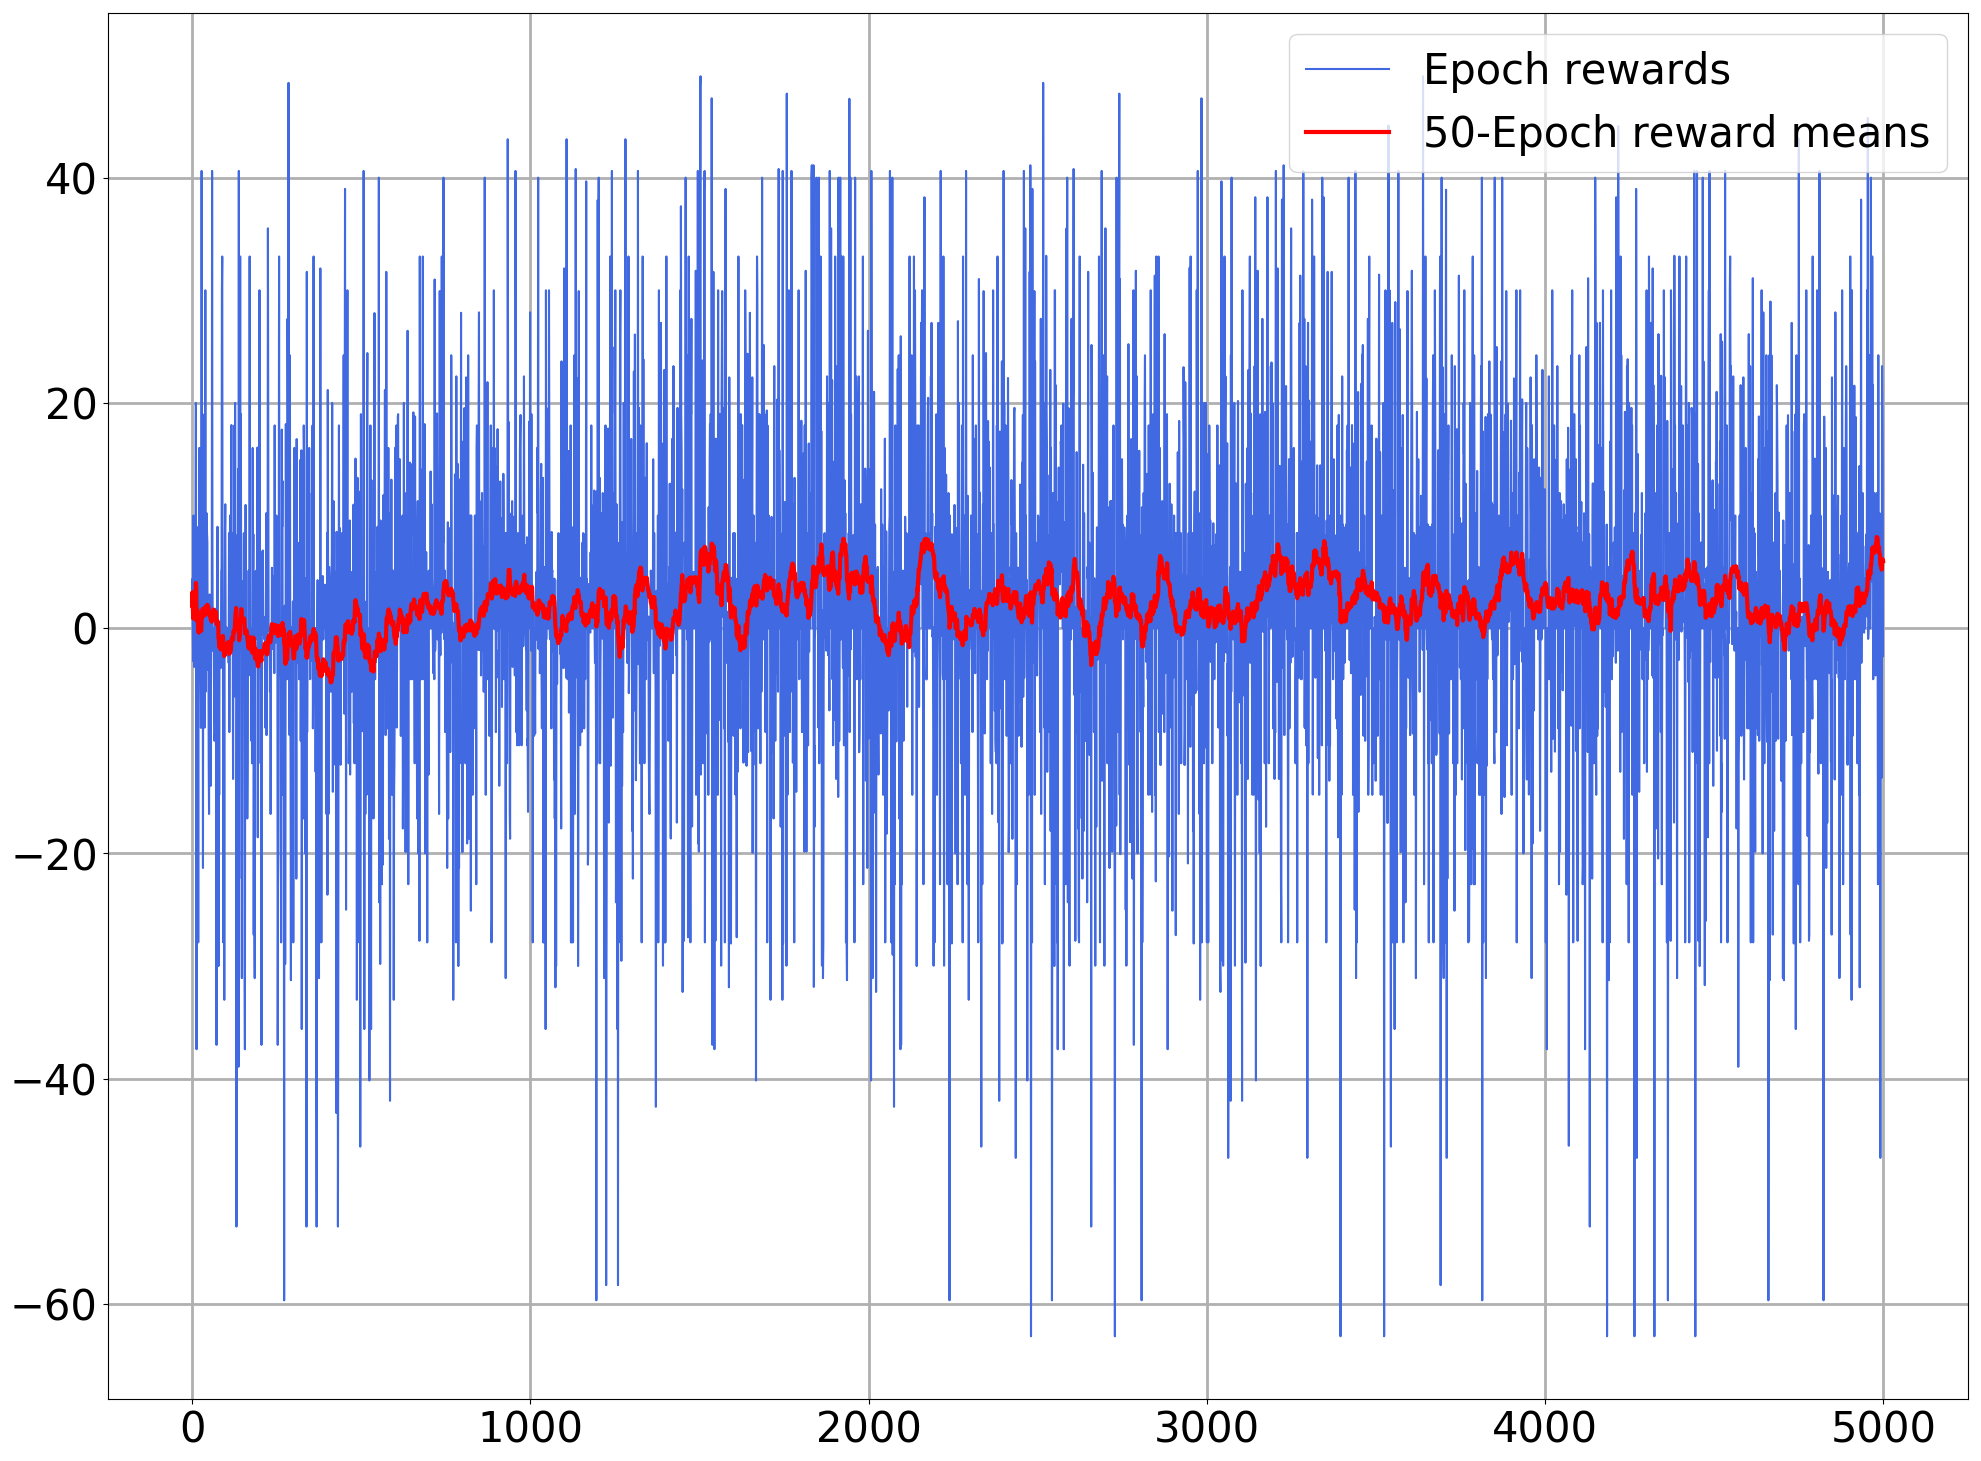
\includegraphics[width=\textwidth]{cnn_2_sell_rewards.png}
        \caption{Mean rewards per epoch (sell)}
        \label{fig:analysis-dqn-2-reward-sell}
    \end{subfigure}
    \begin{subfigure}[b]{0.4\textwidth}
        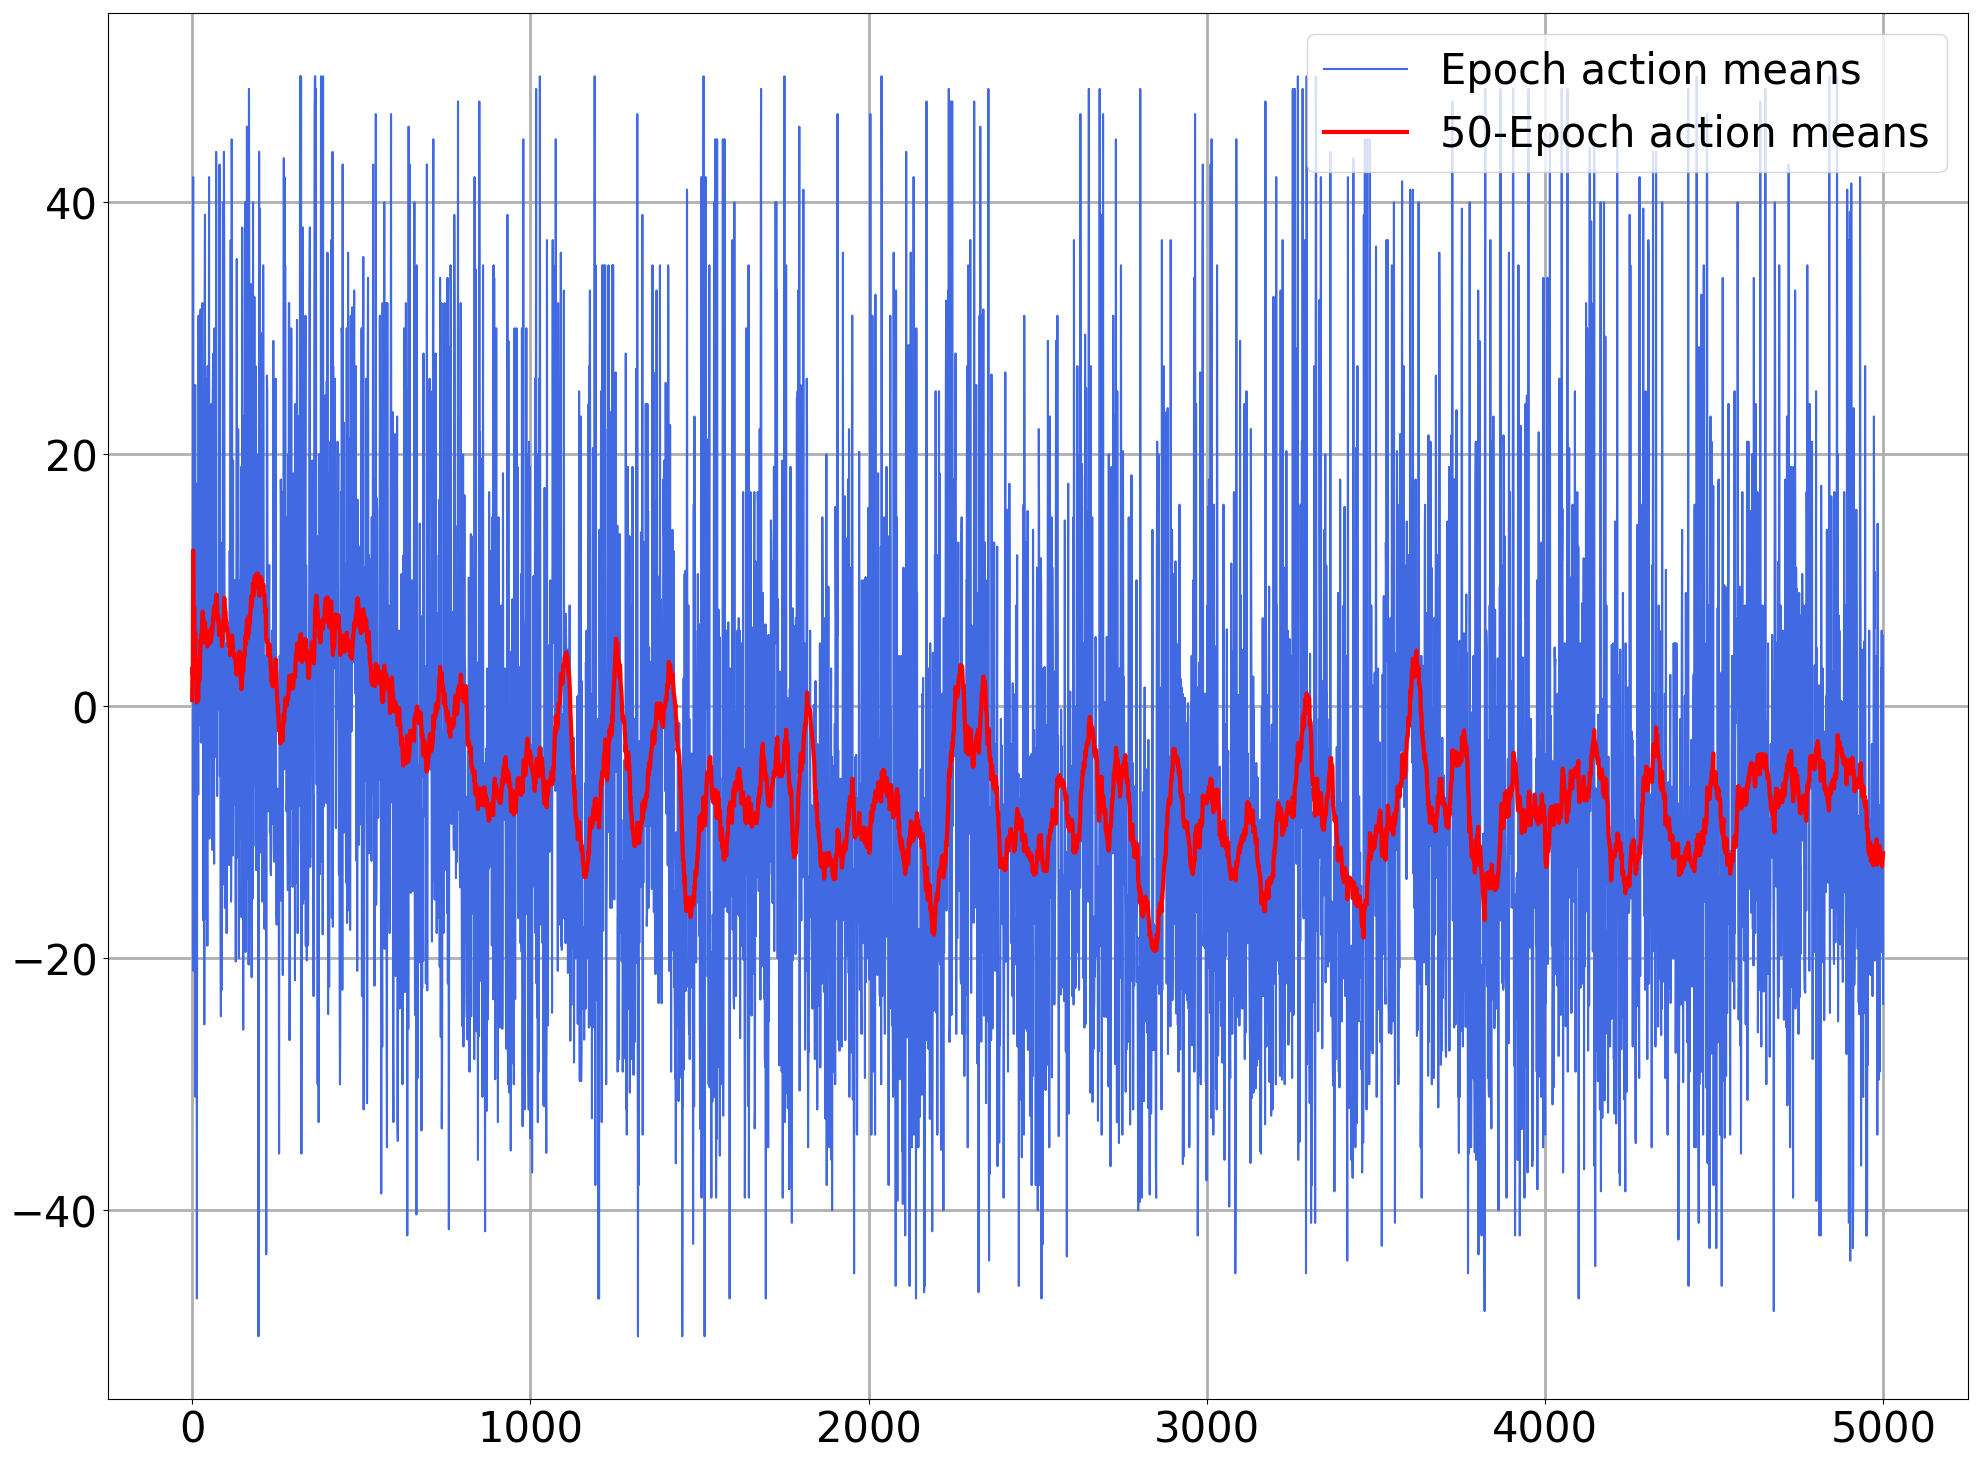
\includegraphics[width=\textwidth]{cnn_2_sell_mean_actions.png}
        \caption{Mean of actions per epoch (sell)}
        \label{fig:analysis-dqn-2-action-sell}
    \end{subfigure}
    \caption{DQN agent rewards and mean of actions for buying and selling on training data set II using feature I.}
    \label{fig:analysis-dqn-2}
\end{figure}

Figure \ref{fig:analysis-dqn-1} shows the learning process using the data set I.
During the training process of buying assets, the received rewards were consistently improve over the course of the 5000 epochs (Figure \ref{fig:analysis-dqn-1-reward-buy}), throughout which the agent steadily adjusted the actions to be chosen more negatively (Figure \ref{fig:analysis-dqn-1-action-buy}).
After 2000 epochs, the average chosen action stagnated just below -20, which is \$2.00 below the market price.
It is evident that this adjustment is not as linear as during the training of the Q-Learning agent as shown in the previous section.
However, the adjustment is appropriate since the market price was falling.
Therefore, the achieved reward during the backtest resulted in 22.06, which is a significant improvement compared to the expected return of -0.05 for a market order.

The received rewards for selling is shown in Figure \ref{fig:analysis-dqn-1-reward-sell} and the average chosen action throughout the epochs is shown in Figure \ref{fig:analysis-dqn-1-action-sell}.
The rewards were not improved over the course of the training and the agent did not choose to adjust the actions on average.
Possibly, this is due to the constant negative rewards received during the training under the difficult market conditions for selling assets while the market price is falling.
As a result, during the backtest a negative reward of -39.26 was achieved, much worse than a market order which comes with the expected return of -27.70 and therefore indicate that the agent despite the fact of a falling market tried to sell with limit orders instead of market orders.

Figure \ref{fig:analysis-dqn-2} shows the agents learning process using the data set II.
Over the course of 5000 epochs the agent was not able to improve its reward and instead stagnated on average at approximately \$0.00 rewards per epoch, as shown in Figure \ref{fig:analysis-dqn-2-reward-buy}.
The agent adjusted the chosen actions steadily such that the average limit level was below -20 at epoch 2000 and remained at this level, as shown in Figure \ref{fig:analysis-dqn-2-action-buy}.
Therefore the reward was a product of market orders as the orders with these limit levels were most likely not filled.
After all, the backtest resulted in an average reward of -2.26 which is, compared to the expected market order reward of -1.06, slightly worse.

The rewards for the agent that learned to sell assets is shown in Figure \ref{fig:analysis-q-learn-2-reward-sell}.
The reward could not be improved during the training, even though the agent lowered the average action chosen below -20, as shown in Figure \ref{fig:analysis-q-learn-2-action-sell}.
Under this uprising market condition, the observed rewards are a product of the market order, since negative actions will likely not result in a filled order.

The rewards for selling assets under the rising market conditions could be improved and, after 1000 training epochs, kept constantly above \$0.00, as shown in Figure \ref{fig:analysis-q-learn-2-reward-sell}.
Therefore, the average of actions chosen for an epoch was lowered within the first 1000 epochs and, going forward, remained at approximately -10, which correlates with the received rewards.
Finally, the backtest resulted in an average reward of 0.84, which is an improvement compared to the expected reward of -1.72 for a market.
\\
\\
Table \ref{tbl:analysis-dqn-orderfeature-summary} summarizes the average rewards observed during the backtest using the DQN agent that uses Feature I, which includes 30 historical order book states as features and therefore has knowledge about the change in created and cancelled orders.
Overall, the DQN agent was able to optimize limit order placement when the given market conditions came in favor of making a purchase or sale respectively.
More precisely, significant improvements were made when the task was to buy assets and the market price was falling and minor optimization was achieved when the task was to sell assets and the market price was rising.
Under these conditions, the DQN agent performed better than the Q-Learning agent.
However, when market conditions did not come in favor of the intention to either buy or sell respectively, the agent performed not only worse than the expected return of a market order but also worse than the Q-Learning agent.
\begin{table}[H]
\centering
\begin{tabular}{l|l|l|}
\cline{2-3}
& \textbf{DQN (Feature I)} & \textbf{\begin{tabular}[c]{@{}l@{}}$\mathbb{E}$[Market\\ Order]\end{tabular}} \\ \hline
\multicolumn{1}{|l|}{\textbf{Buy (I)}}   & 22.06          & -0.05                                                           \\ \hline
\multicolumn{1}{|l|}{\textbf{Sell (I)}}  & -39.26         & -27.70                                                          \\ \hline
\multicolumn{1}{|l|}{\textbf{Buy (II)}}  & -2.26          & -1.06                                                           \\ \hline
\multicolumn{1}{|l|}{\textbf{Sell (II)}} & 0.84          & -1.72                                                           \\ \hline
\end{tabular}
\caption{Summary of rewards during backtest of DQN agent using Feature I (historical orders).}
\label{tbl:analysis-dqn-orderfeature-summary}
\end{table}

\subsection{Application of historical trade feature}

The following evaluation of the DQN agent considers historical trades as described in Chapter \ref{chap:data} (Section \ref{sec:data-feature-2}) which we denote henceforth as Feature II.
Therefore, a \textit{lookback} of 30 trades are considered.
Consequently this feature set is of size: $(lookback, 4) \implies (30, 3)$.
Including the two private variables that were appended as a vector $[inventory, time, 0, 0]$ at the beginning of this feature vector results a feature set size of: $(31, 4)$ and serves as the input for the CNN.

\begin{figure}[H]
    \centering
    \begin{subfigure}[b]{0.45\textwidth}
        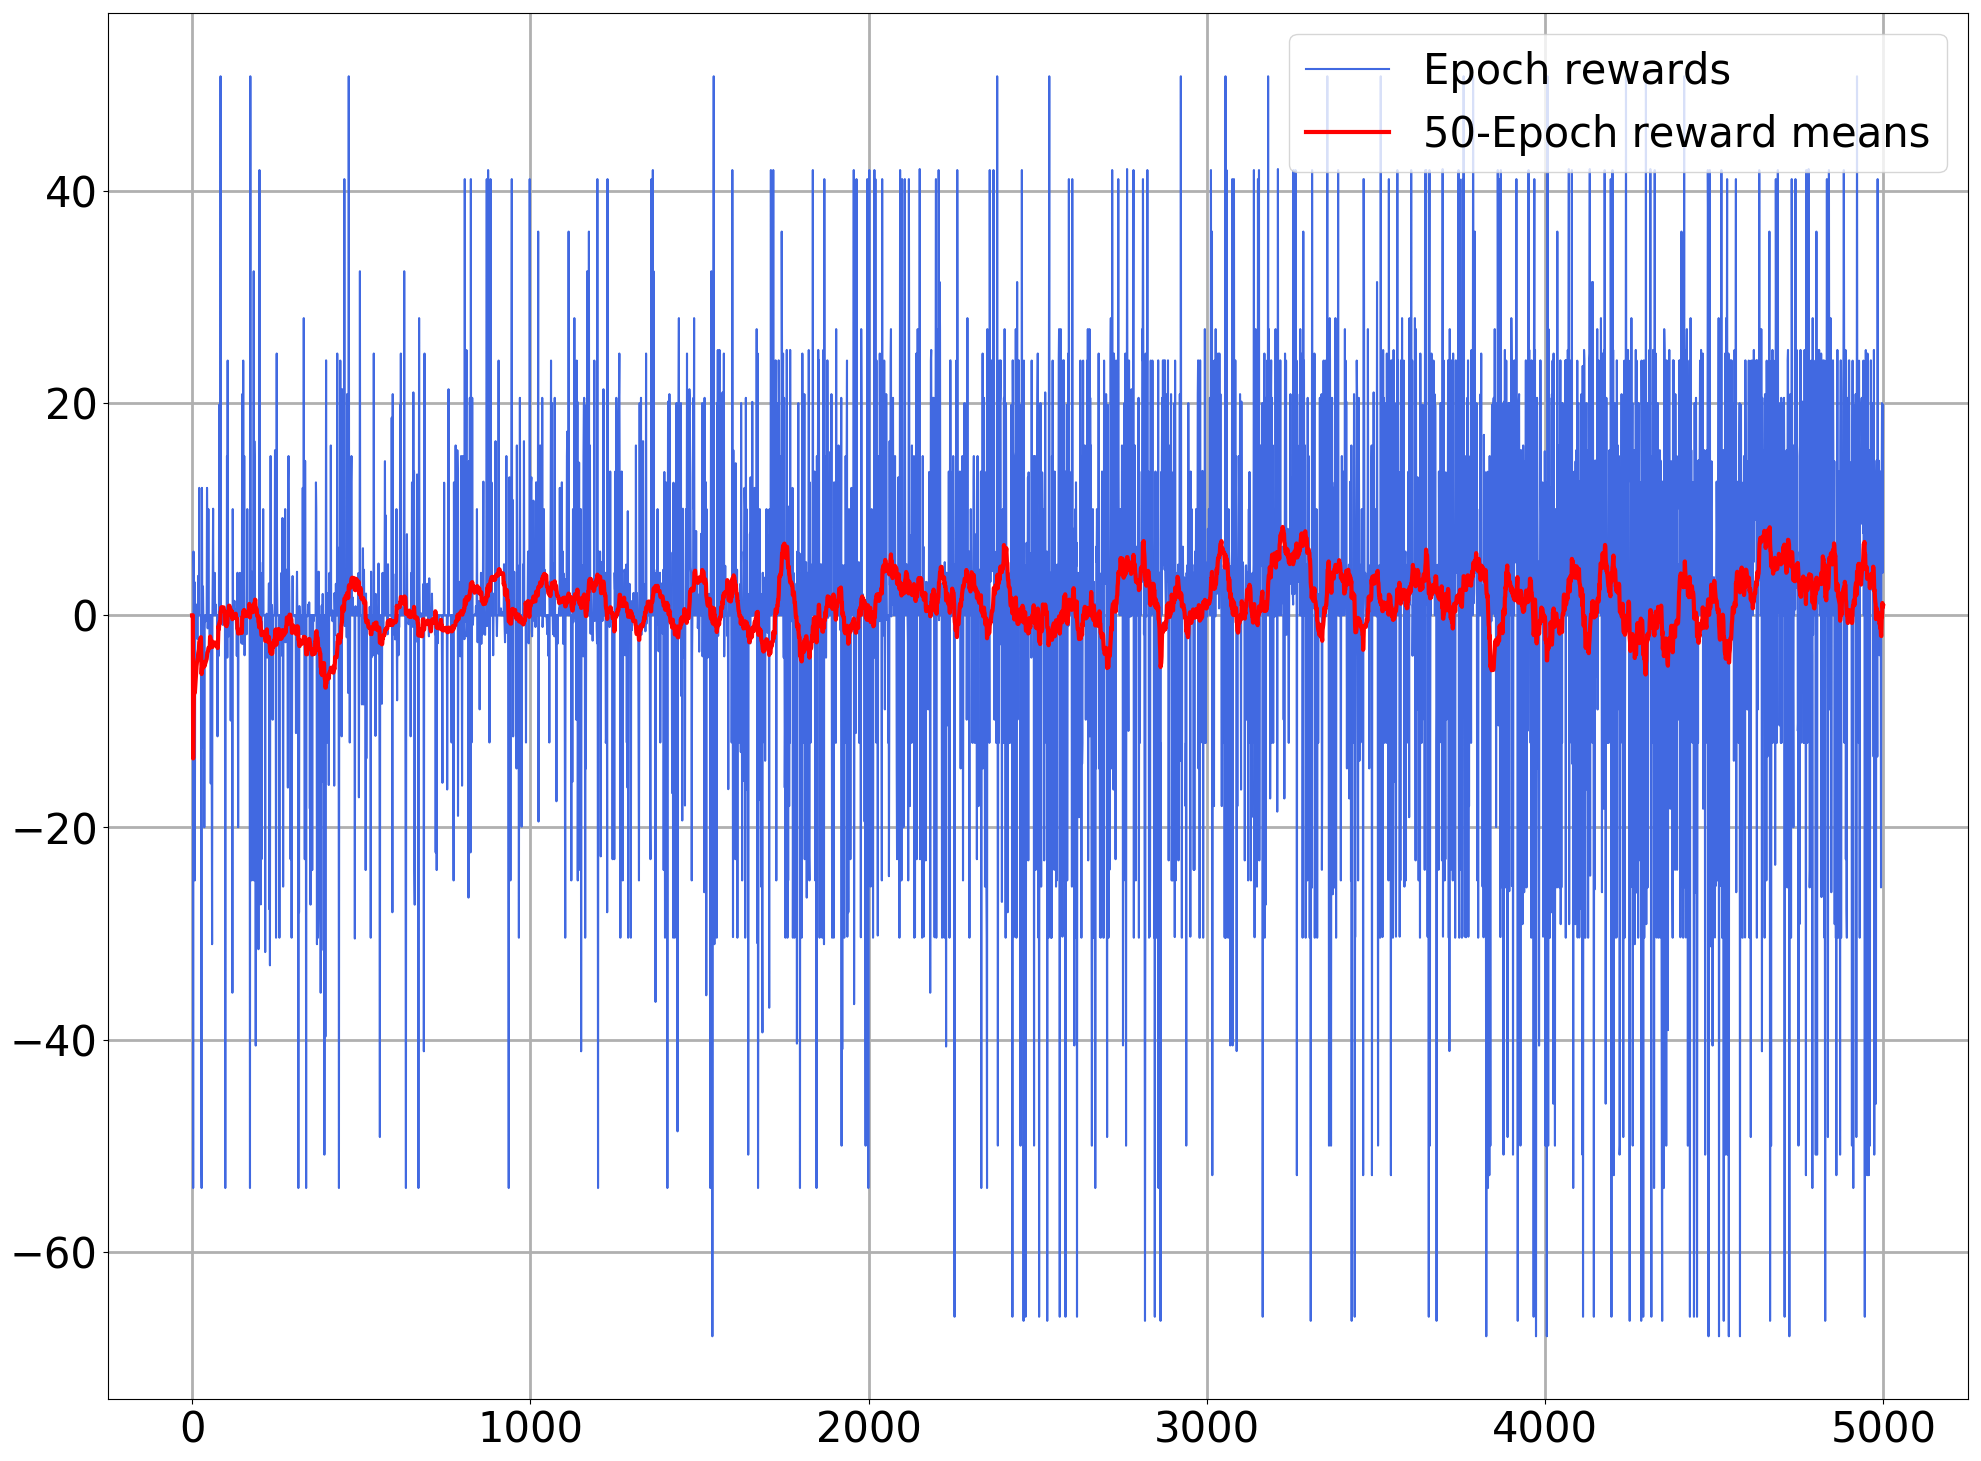
\includegraphics[width=\textwidth]{cnn_1_buy_trades_rewards.png}
        \caption{Reward per epoch (buy)}
        \label{fig:analysis-dqn-1-trades-reward-buy}
    \end{subfigure}
    \begin{subfigure}[b]{0.45\textwidth}
        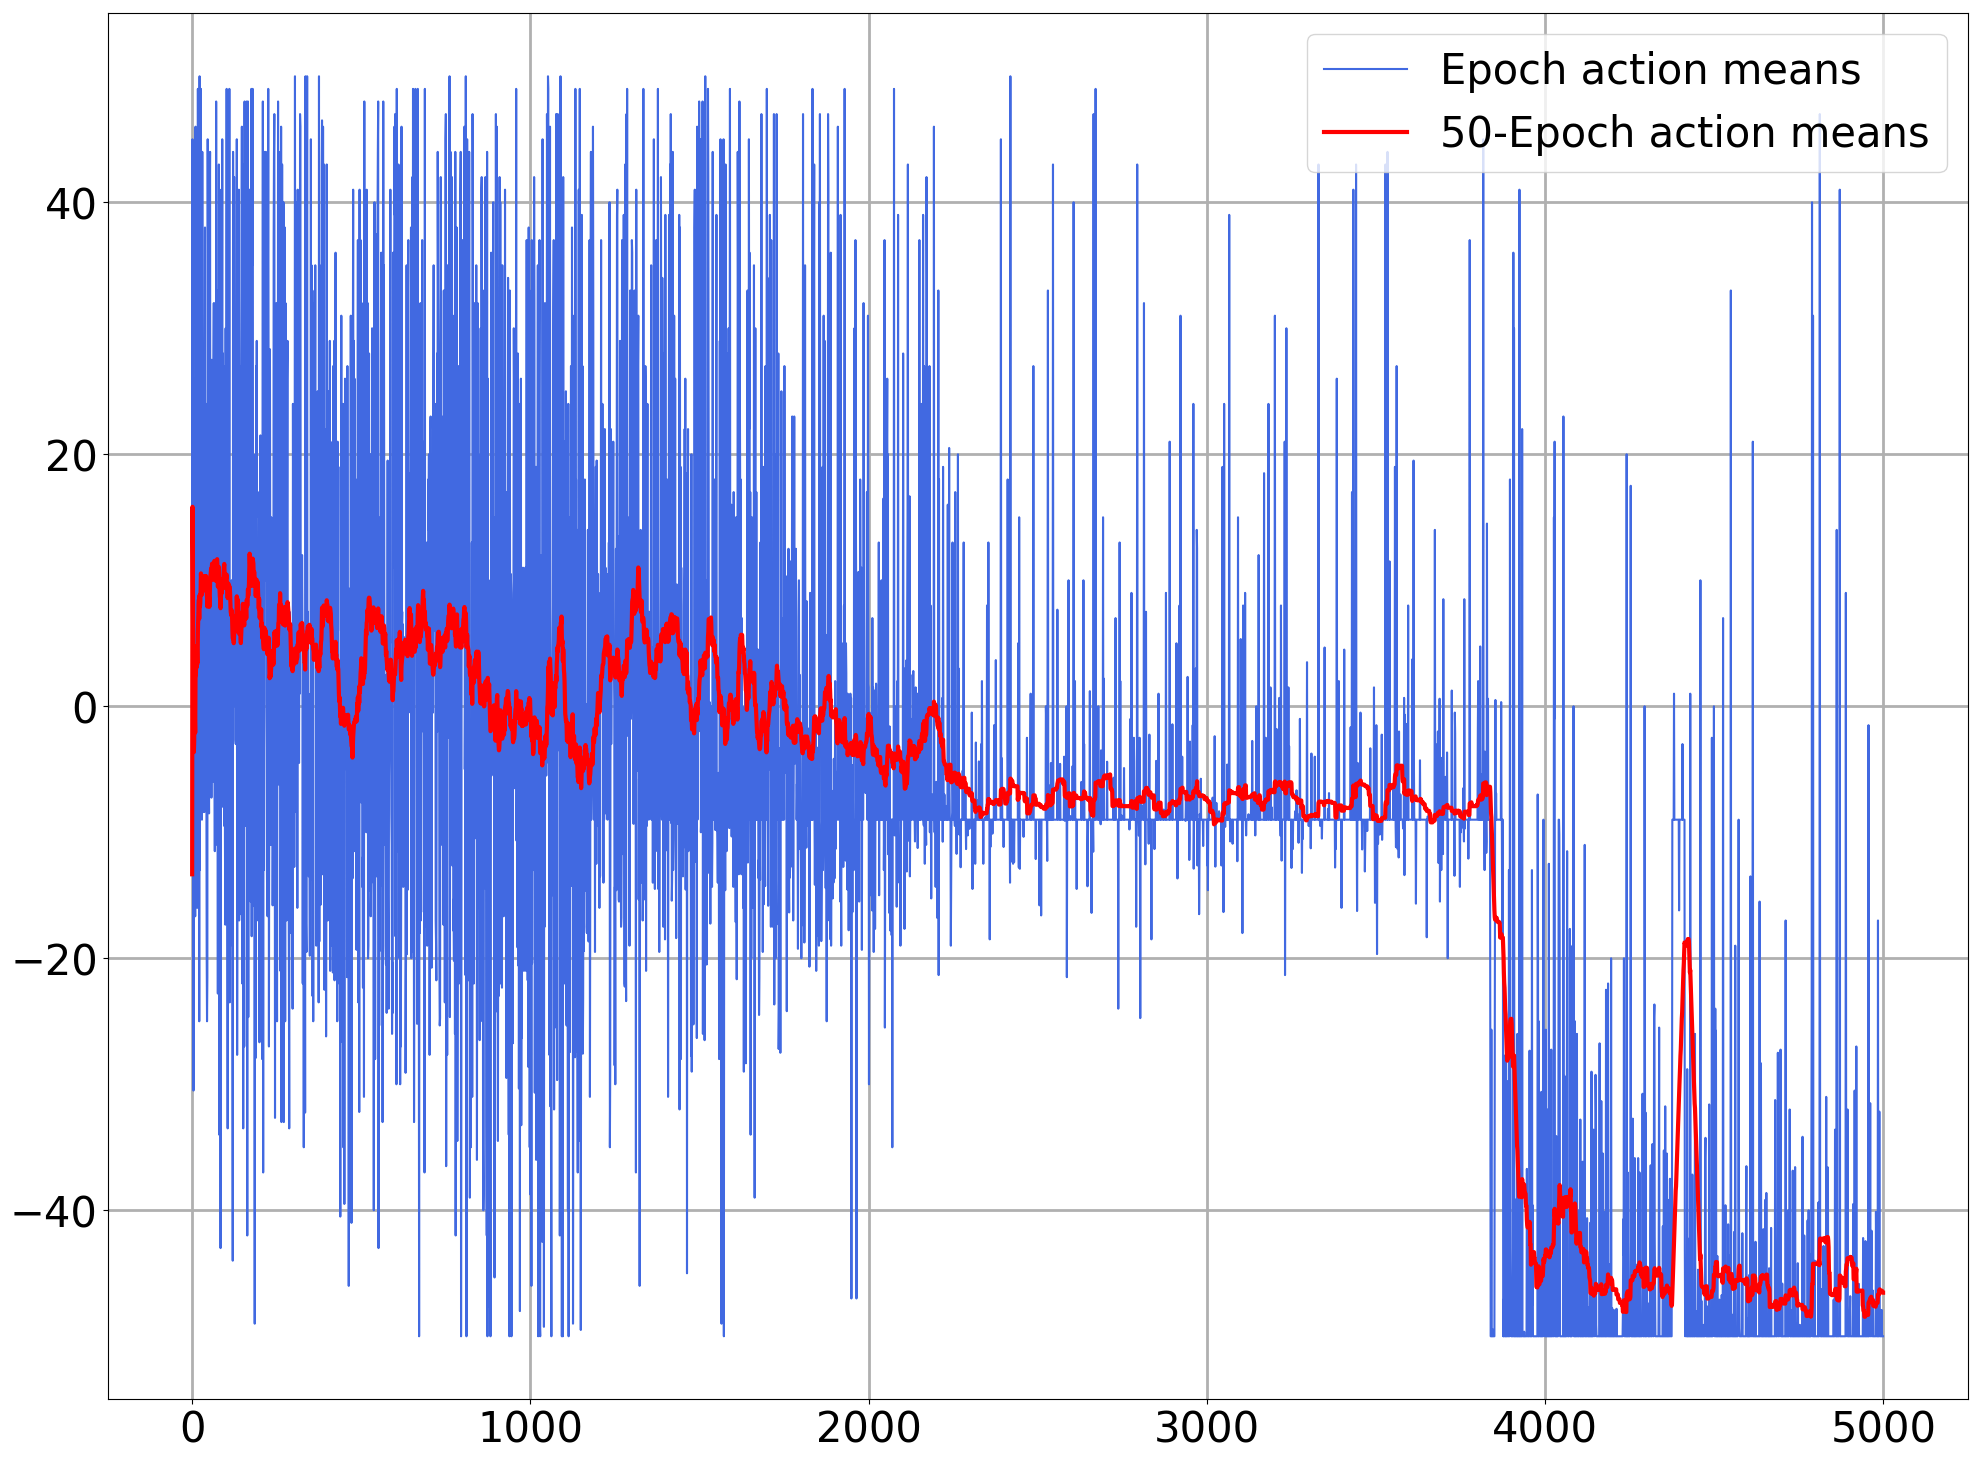
\includegraphics[width=\textwidth]{cnn_1_buy_trades_mean_actions.png}
        \caption{Mean of actions per epoch (buy)}
        \label{fig:analysis-dqn-1-trades-action-buy}
    \end{subfigure}
    \begin{subfigure}[b]{0.45\textwidth}
        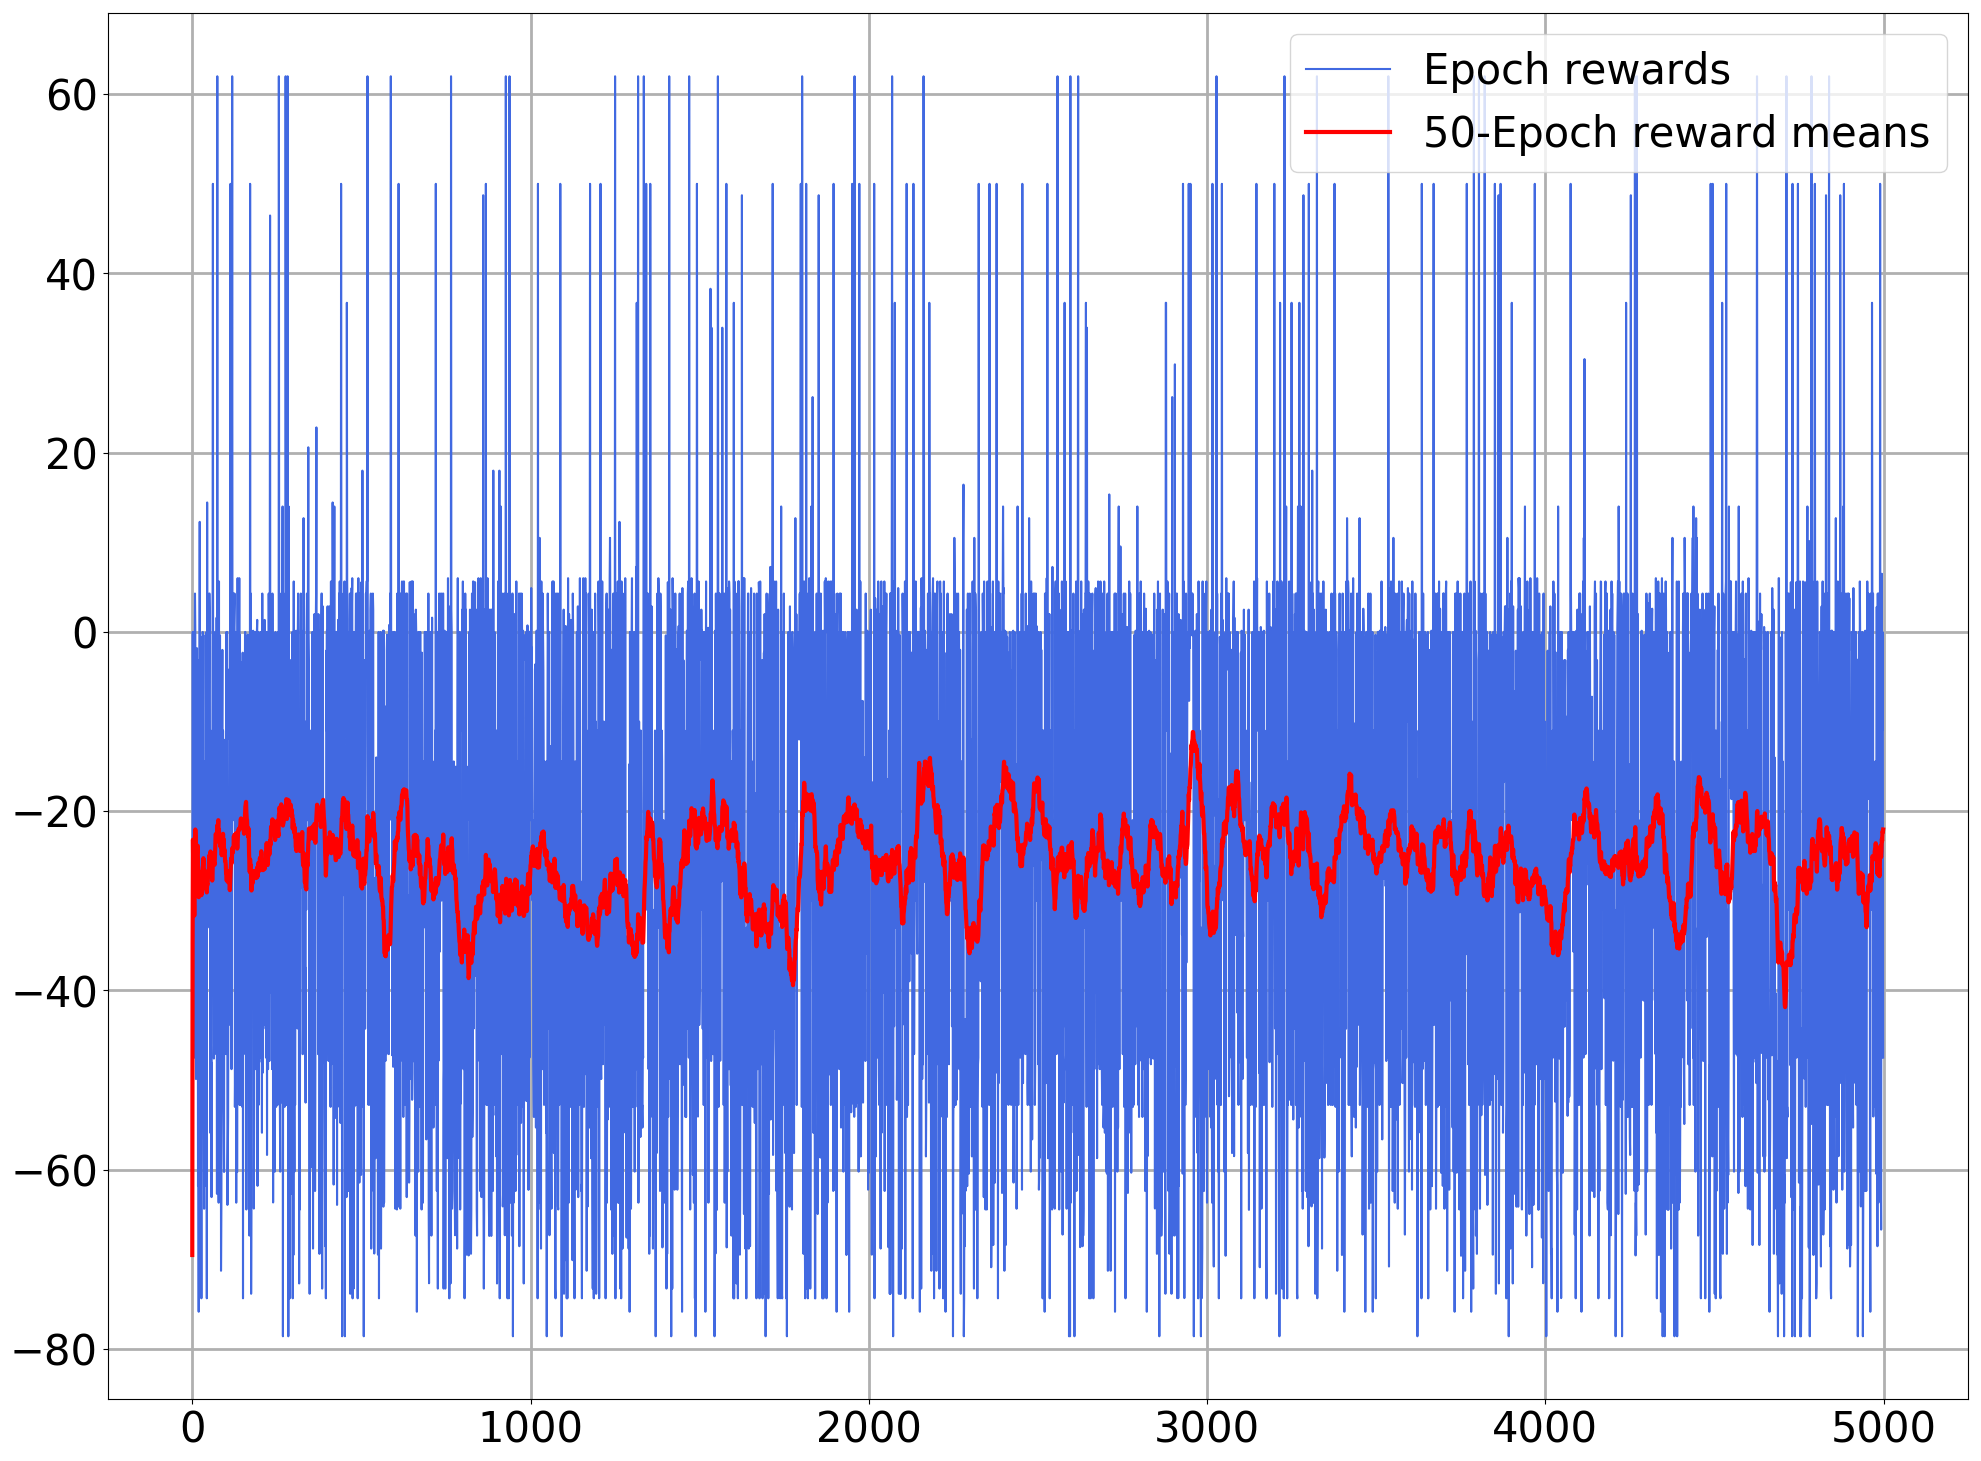
\includegraphics[width=\textwidth]{cnn_1_sell_trades_rewards.png}
        \caption{Mean rewards per epoch (sell)}
        \label{fig:analysis-dqn-1-trades-reward-sell}
    \end{subfigure}
    \begin{subfigure}[b]{0.45\textwidth}
        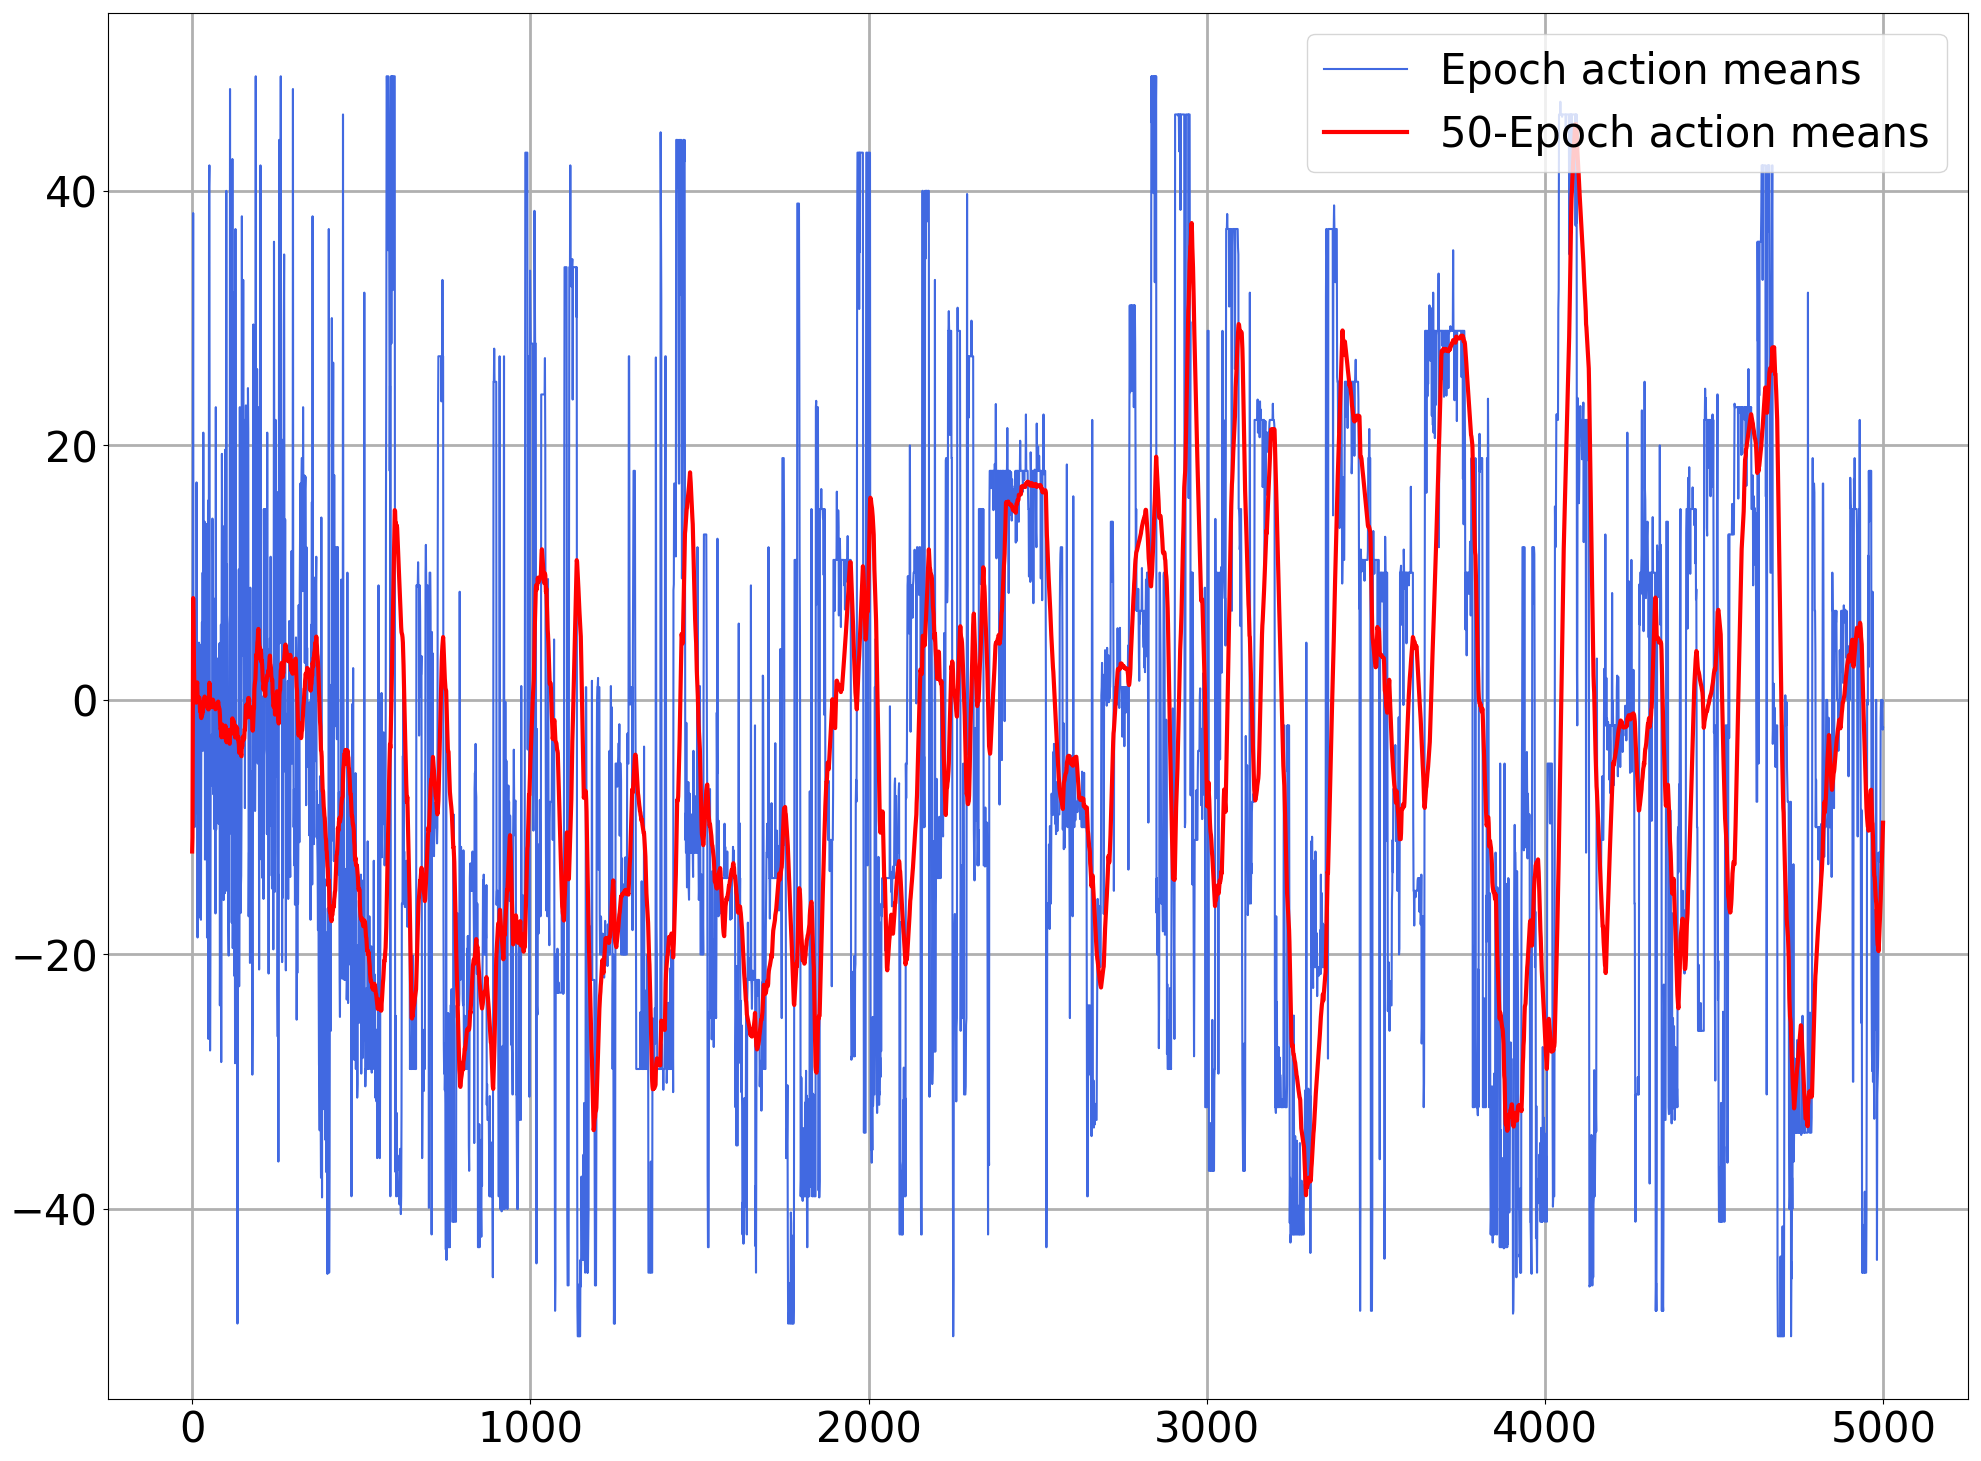
\includegraphics[width=\textwidth]{cnn_1_sell_trades_mean_actions.png}
        \caption{Mean of actions per epoch (sell)}
        \label{fig:analysis-dqn-1-trades-action-sell}
    \end{subfigure}
    \caption{DQN agent rewards and mean of actions for buying and selling on training data set I using feature II.}
    \label{fig:analysis-dqn-1-trades}
\end{figure}

\begin{figure}[H]
    \centering
    \begin{subfigure}[b]{0.45\textwidth}
        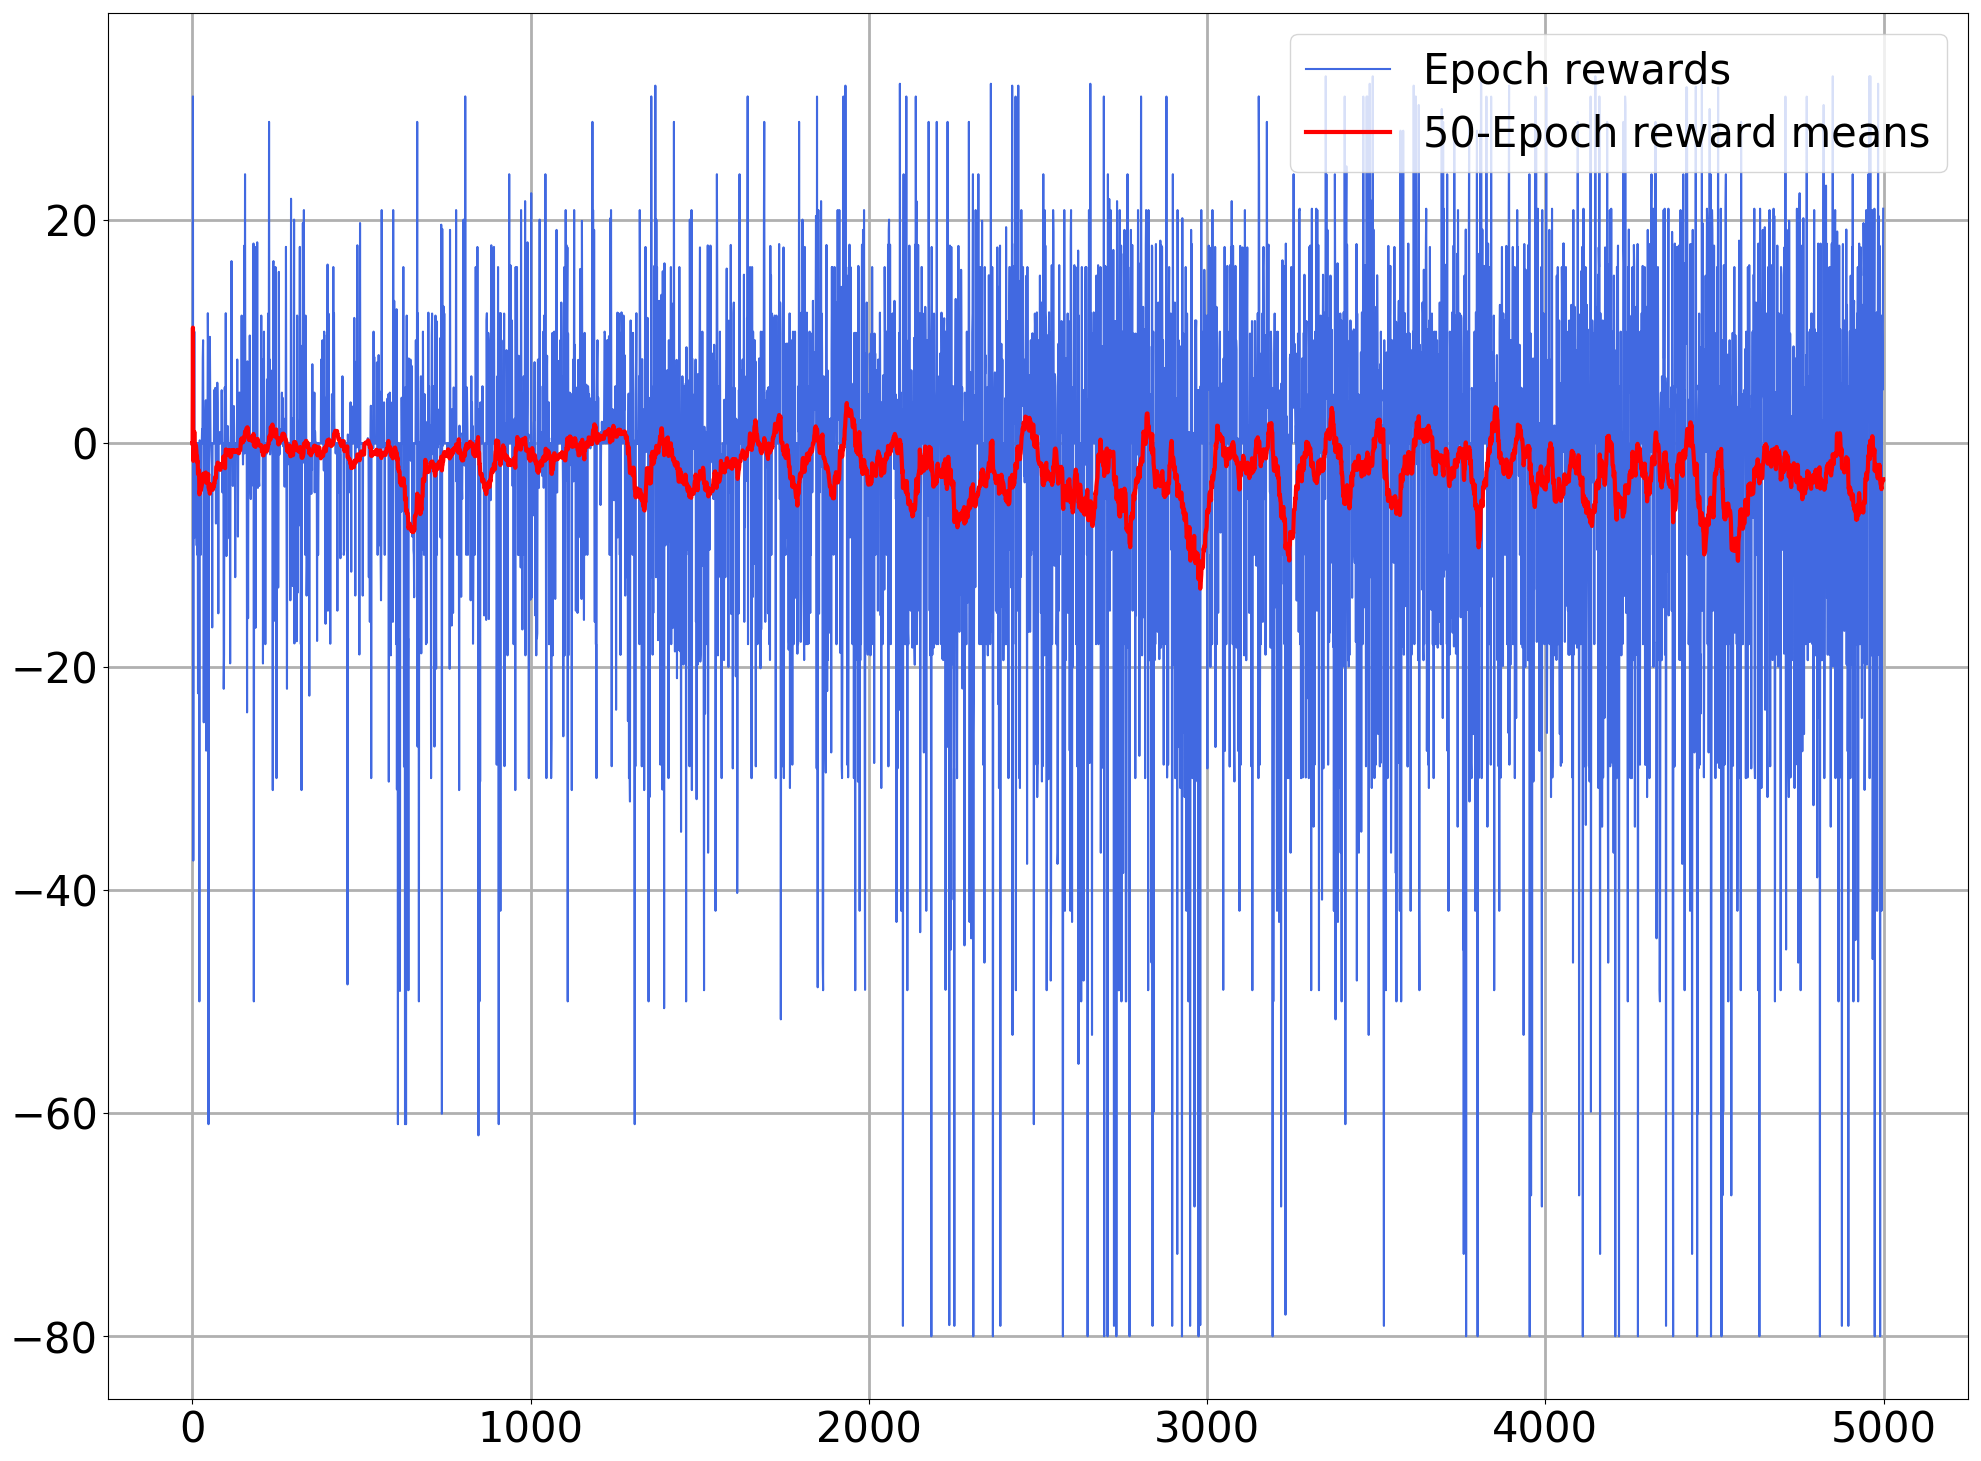
\includegraphics[width=\textwidth]{cnn_2_buy_trades_rewards.png}
        \caption{Reward per epoch (buy)}
        \label{fig:analysis-dqn-2-trades-reward-buy}
    \end{subfigure}
    \begin{subfigure}[b]{0.45\textwidth}
        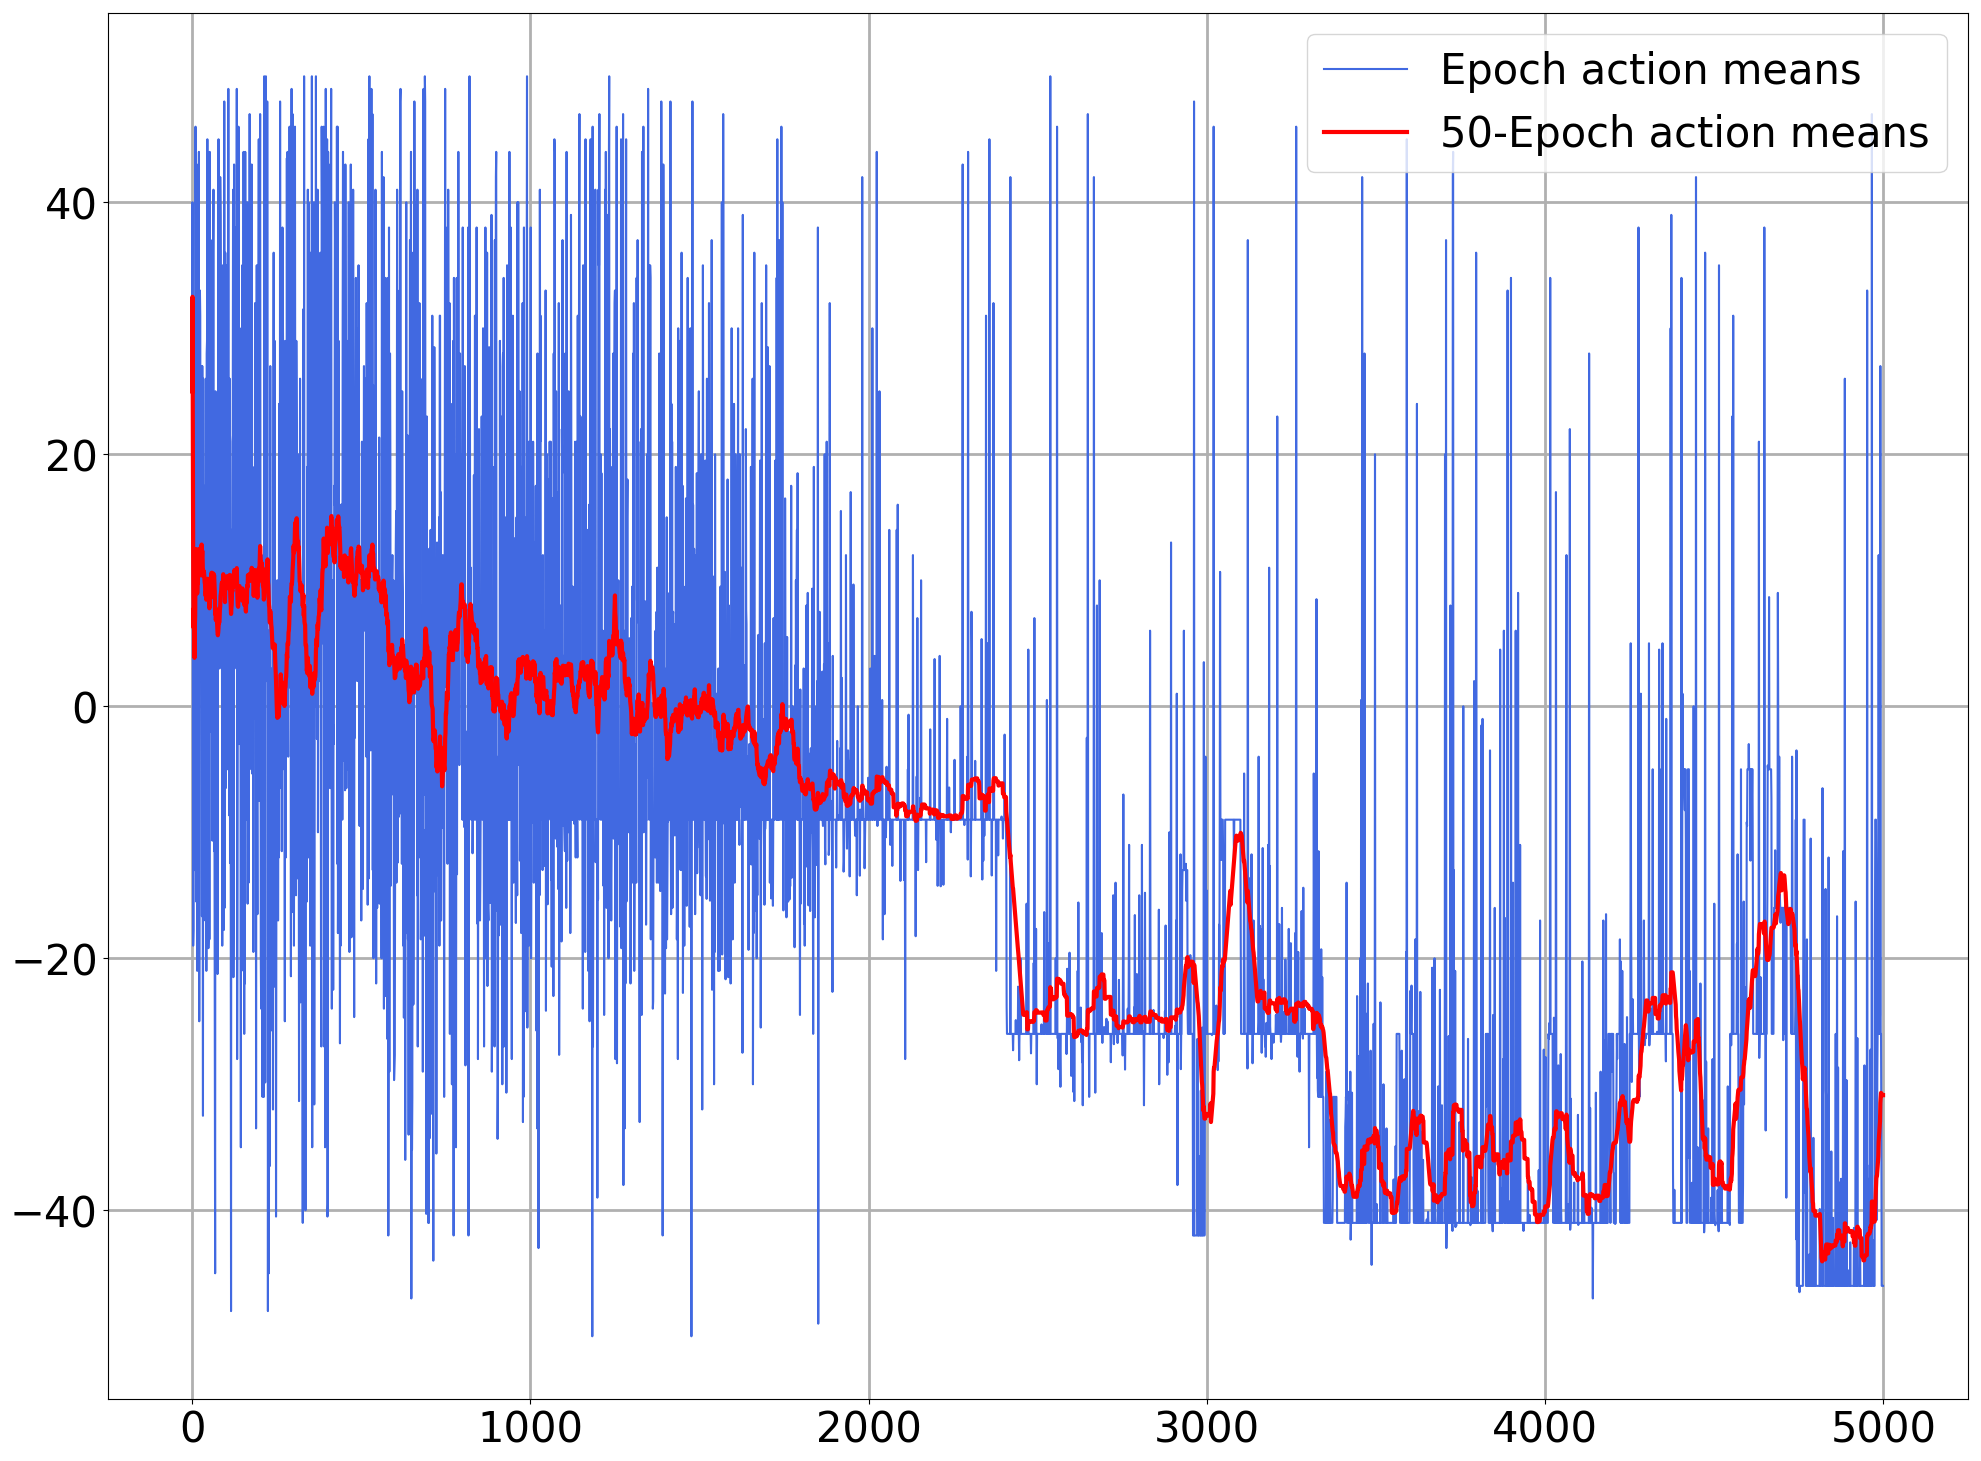
\includegraphics[width=\textwidth]{cnn_2_buy_trades_mean_actions.png}
        \caption{Mean of actions per epoch (buy)}
        \label{fig:analysis-dqn-2-trades-action-buy}
    \end{subfigure}
    \begin{subfigure}[b]{0.45\textwidth}
        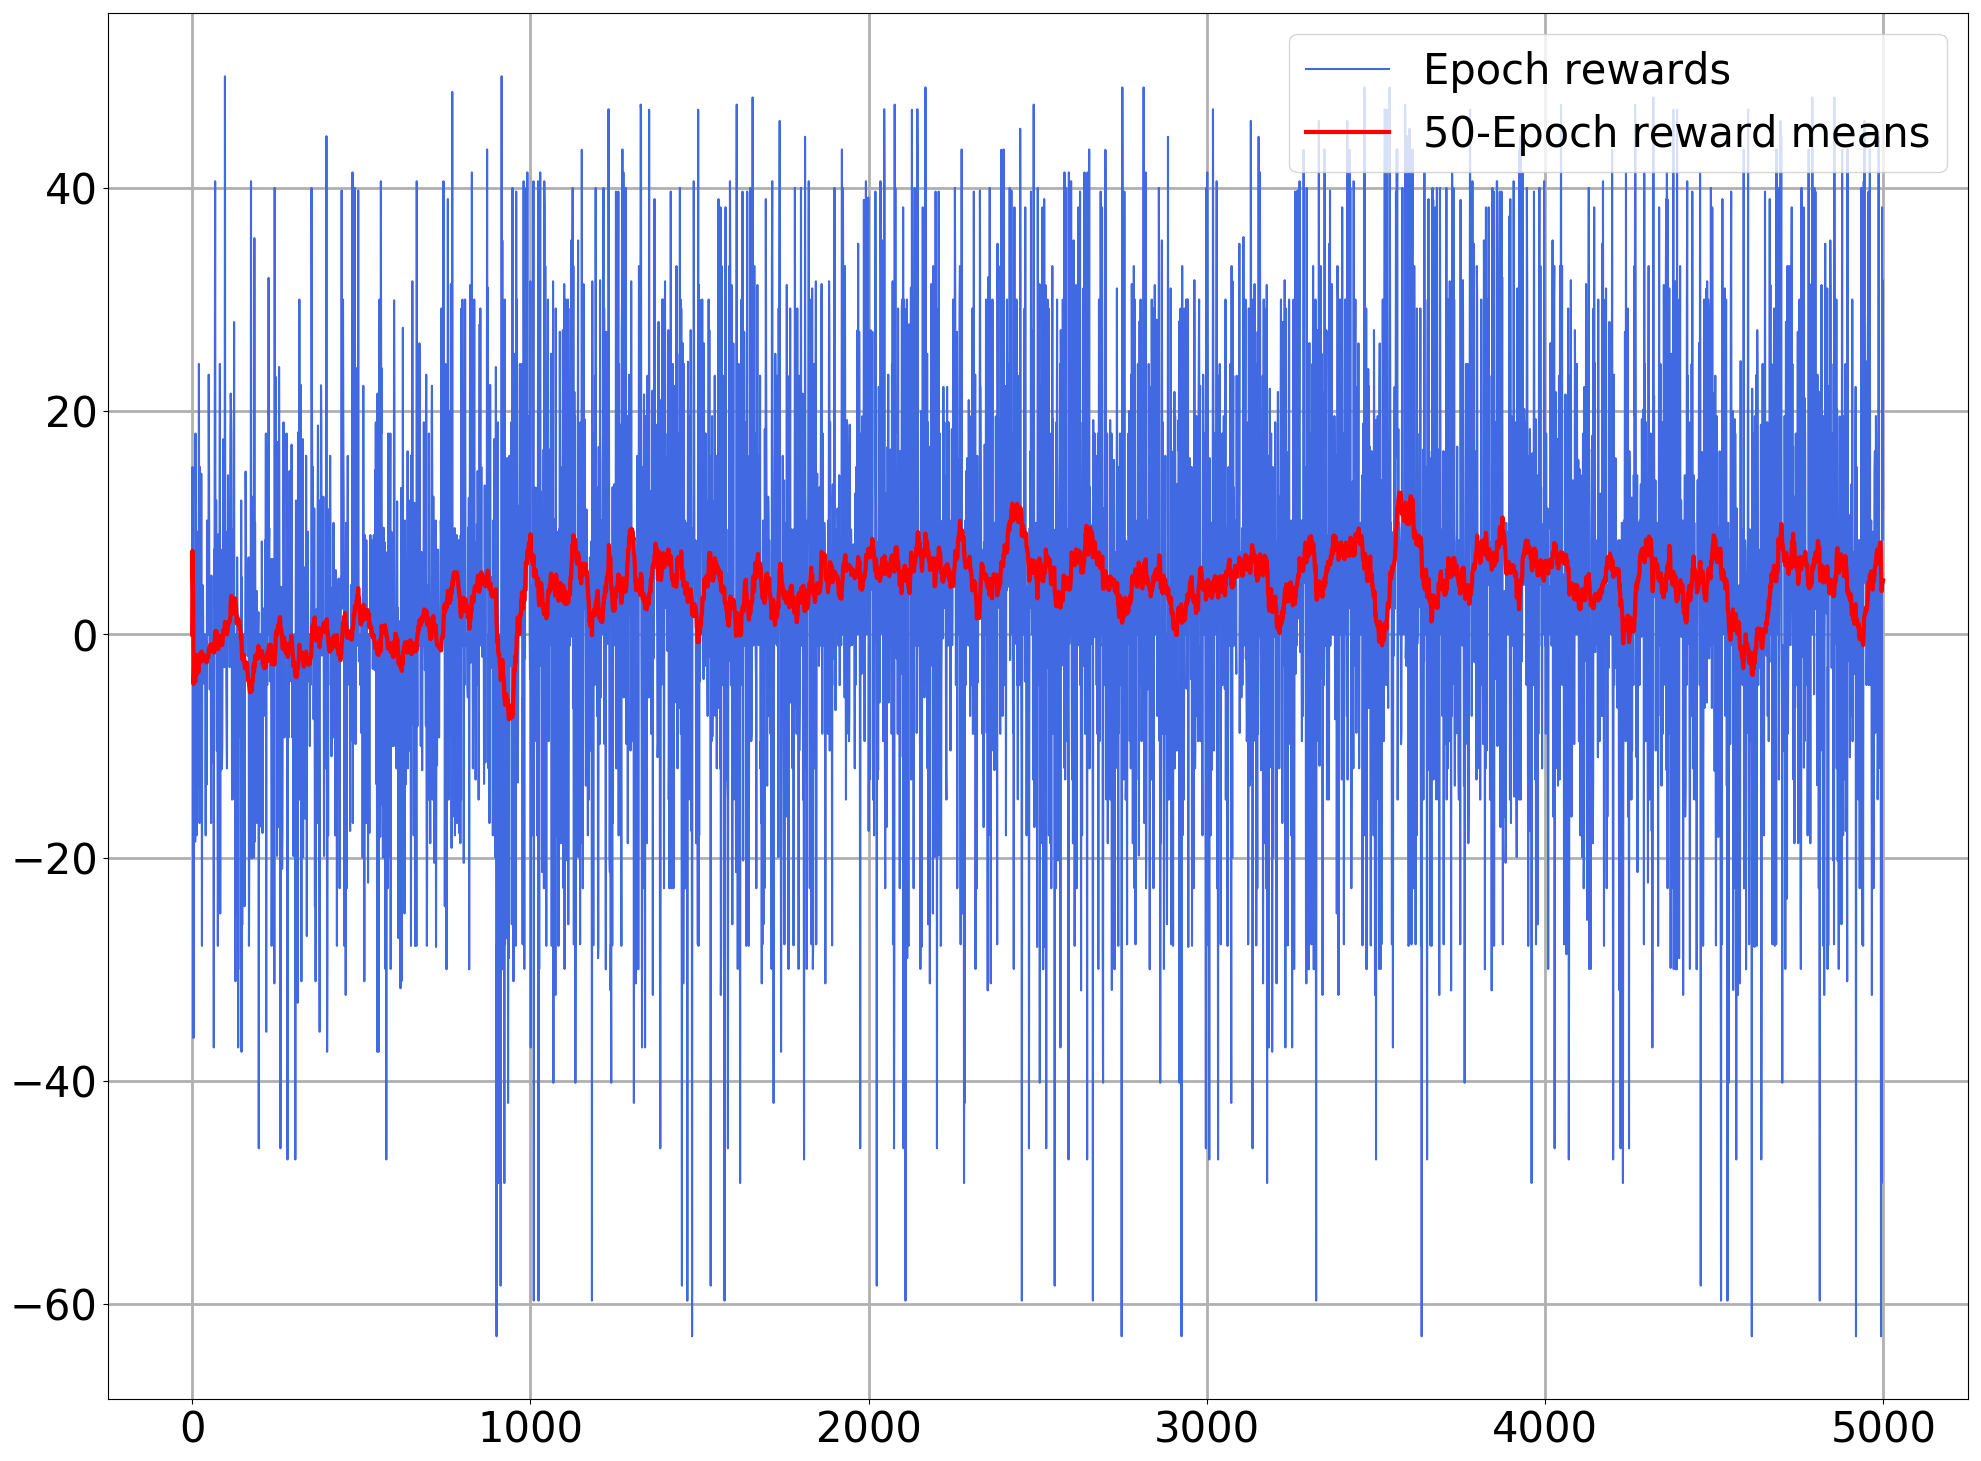
\includegraphics[width=\textwidth]{cnn_2_sell_trades_rewards.png}
        \caption{Mean rewards per epoch (sell)}
        \label{fig:analysis-dqn-2-trades-reward-sell}
    \end{subfigure}
    \begin{subfigure}[b]{0.45\textwidth}
        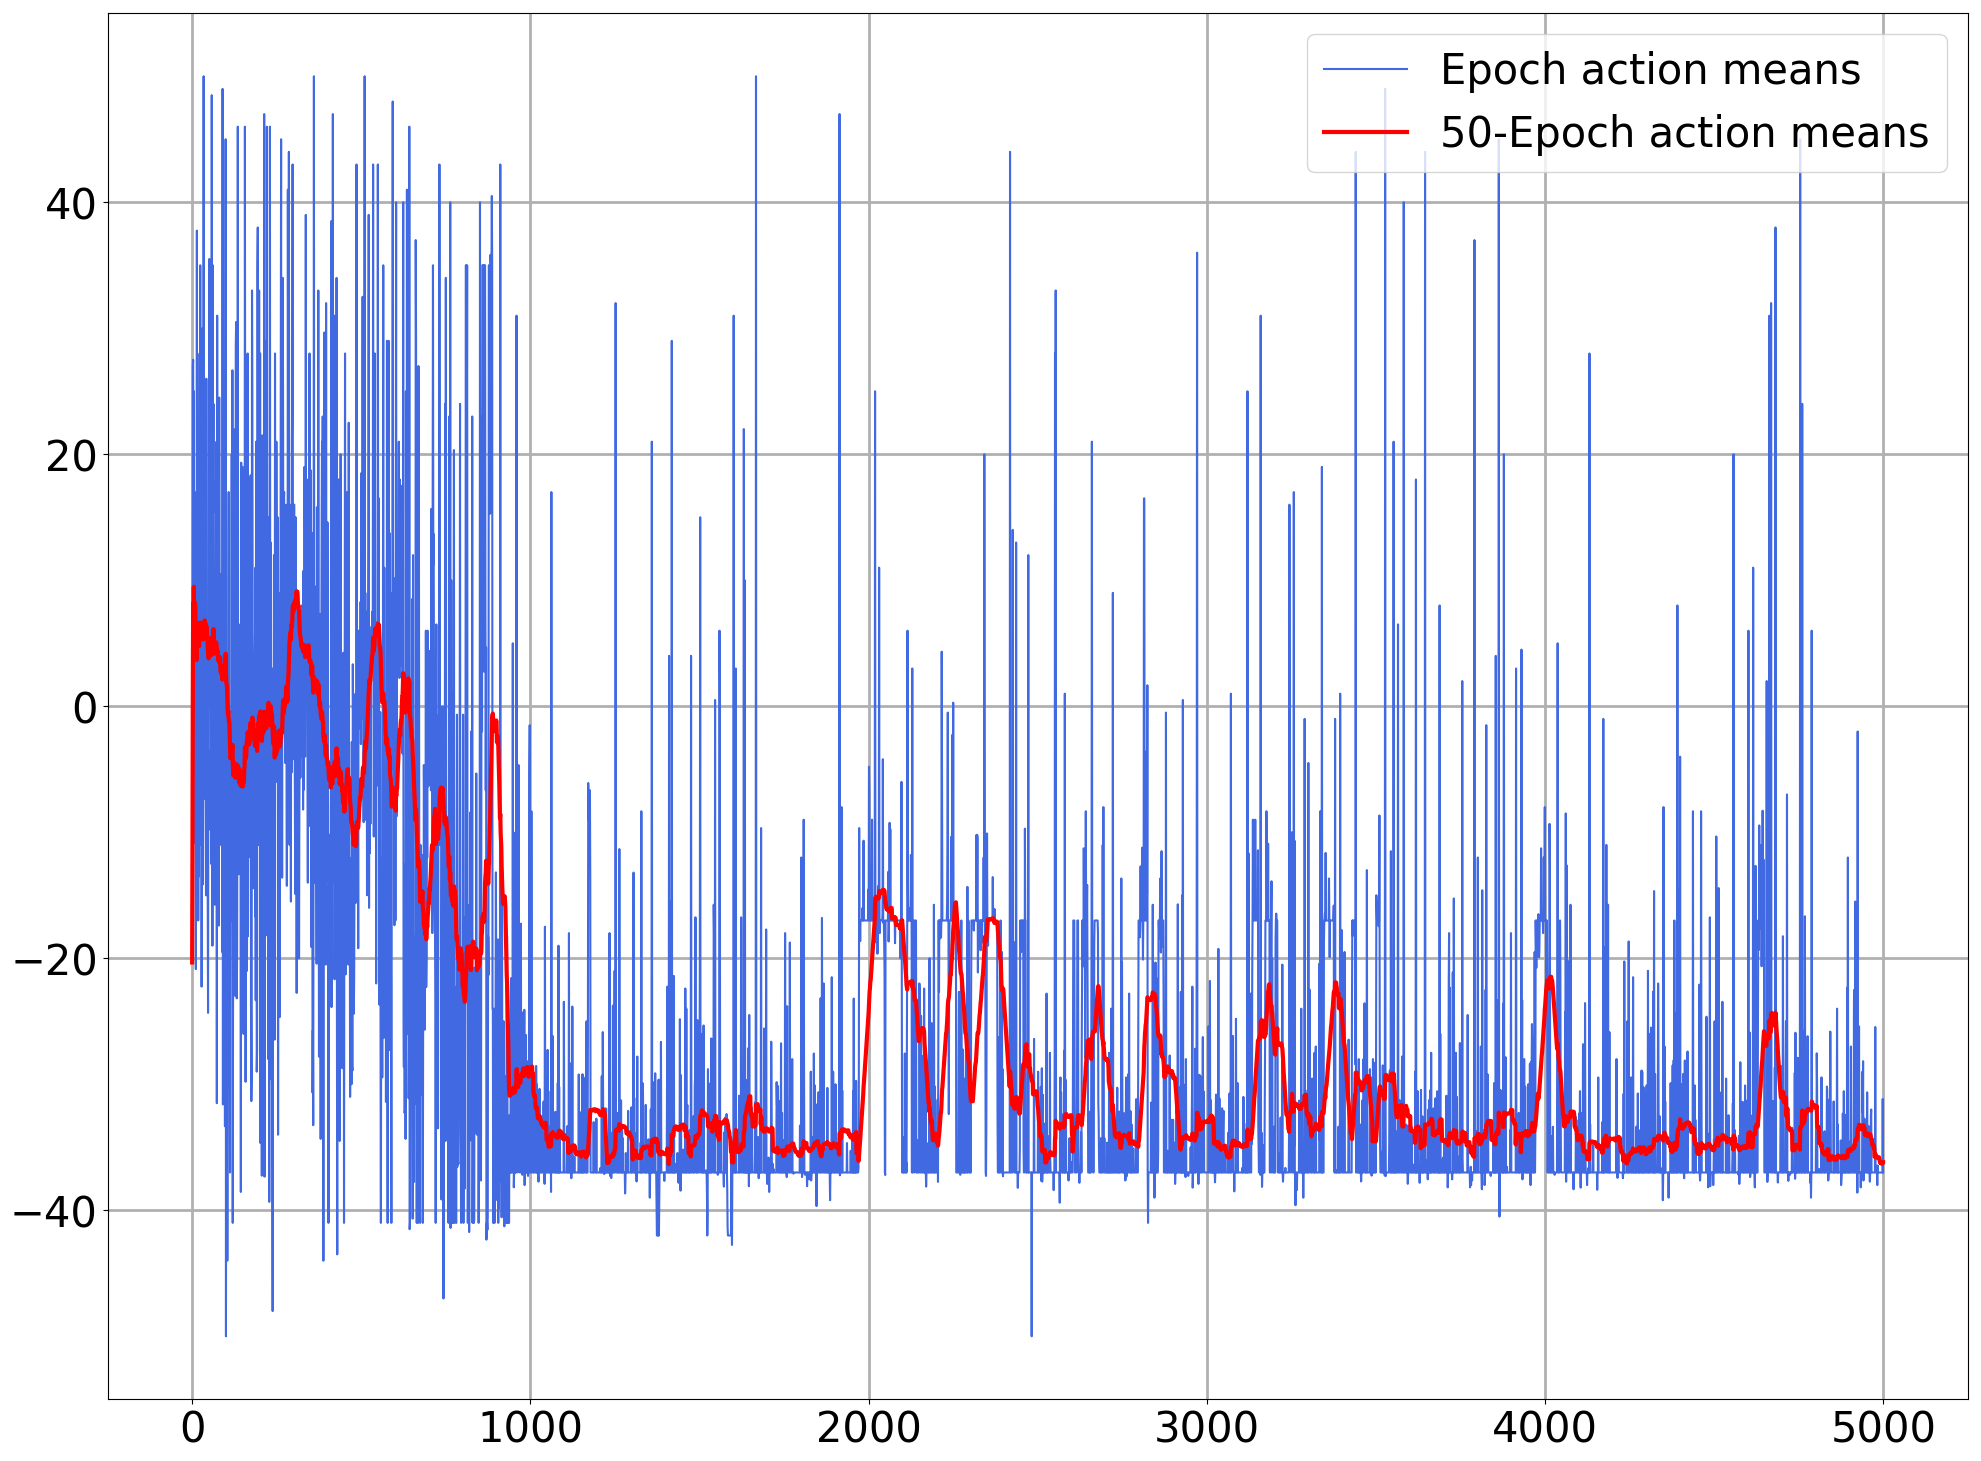
\includegraphics[width=\textwidth]{cnn_2_sell_trades_mean_actions.png}
        \caption{Mean of actions per epoch (sell)}
        \label{fig:analysis-dqn-2-trades-action-sell}
    \end{subfigure}
    \caption{DQN agent rewards and mean of actions for buying and selling on training data set II using feature II.}
    \label{fig:analysis-dqn-2-trades}
\end{figure}

Figure \ref{fig:analysis-dqn-1-trades} illustrates the learning process of the agent for buying and selling using data set I.
Similar to the agent that was provided with Feature I, the rewards received cold be slightly improved over the course of 5000 epochs, as shown in Figure \ref{fig:analysis-dqn-1-trades-reward-buy}.
Interestingly, the average action per epoch converged just below -40 after an abrupt adjustment was made after 4000 epochs.
The average reward achieved during the backtest is 31.92 and is a clear improvement compared to the expected market order return of -0.05.

The rewards received for selling remained at -20, as shown in Figure \ref{fig:analysis-dqn-1-trades-reward-sell}.
However, the average of the actions chosen remain volatile and no clear trend can be seen in Figure \ref{fig:analysis-dqn-1-trades-action-sell}.
This is by no means a negative sign, perhaps the agent indeed learned to respond on distinct patterns with appropriate measures.
As a result, during the backtest an average reward of -35.15 was achieved, which is still worse than the expected return of a market order but significantly better than the DQN agent under the application of Feature I.

Figure \ref{fig:analysis-dqn-2-trades} illustrates the same learning process with the application of data set II.
The rewards for the buying process were not improved (Figure \ref{fig:analysis-dqn-2-trades-reward-buy}) and the actions were adjusted towards limit levels deep in the order book (Figure \ref{fig:analysis-dqn-2-trades-action-buy}).
The backtest resulted in an average reward of -3.56, slightly worse than the expected market return of -1.06.

Rewards for selling increased during the training, as shown in Figure \ref{fig:analysis-dqn-2-trades-reward-sell} and the chosen average action remained just above -40 after 1000 epochs, as shown in Figure \ref{fig:analysis-dqn-2-trades-action-sell}.
The resulted average reward after the backtest was 0.15, which is an improvement to the expected market order return of -1.72.
\\
\\
Table \ref{tbl:analysis-dqn-tradefeature-summary} summarizes the average rewards received for the DQN agent that makes use of Feature II and considers the past 25 trades prior each of the 1000 epochs backtested.
Similar to the previous application of Feature I to the agent, significant optimization could be achieved when market conditions came in favor of buying or selling respectively.
The application of Feature II resulted that the agent was able to outperform the DQN agent with Feature I when it comes to buying when the market price is in tendency to fall.
Slightly worse performance was achieved when attempting to sell and the market price was rising.
Nevertheless the received reward was much better than the expected market order return.
However, when the market conditions came not in favor of the intention to either buy or sell, the agent performed equal to the DQN under application of Feature I.

\begin{table}[H]
\centering
\begin{tabular}{l|l|l|}
\cline{2-3}
& \textbf{DQN (Feature II)} & \textbf{\begin{tabular}[c]{@{}l@{}}$\mathbb{E}$[Market\\ Order]\end{tabular}} \\ \hline
\multicolumn{1}{|l|}{\textbf{Buy (I)}}   & 31.92          & -0.05                                                           \\ \hline
\multicolumn{1}{|l|}{\textbf{Sell (I)}}  & -25.15         & -27.70                                                          \\ \hline
\multicolumn{1}{|l|}{\textbf{Buy (II)}}  & -3.56          & -1.06                                                           \\ \hline
\multicolumn{1}{|l|}{\textbf{Sell (II)}} & 0.15          & -1.72                                                           \\ \hline
\end{tabular}
\caption{Summary of rewards during backtest of DQN agent using Feature II (historical trades).}
\label{tbl:analysis-dqn-tradefeature-summary}
\end{table}

\section{Determining the limitations of the DQN agent}
\label{sec:eval-dqn-limitations}
This section aims to determine the capabilities and limitations of the DQN agent with the use of Feature I in greater detail.
Sample order submissions are investigated which uncover the actions chosen by an agent throughout one epoch.
Therefore, we will be able to see which market situations prevented the agent from achieving a positive reward and conclude why the agent was not able to choose the most ppropriate actions.
In addition, artificial order books are being created which serve as new data sets to train and test the DQN agent on.
By doing so, we aim to determine the capabilities of the deep reinforcement learning technique under market conditions which are 1) not affected by short term fluctuations and 2) a hold constant spread between best bid and best ask is given.

\subsection{Limitation arising from market situations or inappropriate actions from the agent}
Extensive investigations have shown that the DQN agent fails to place orders that lead to constant positive rewards due to the following two reasons: 1) when the market situation does not allow to do so and 2) when the agent submits an inappropriate action.

Our investigations have shown that for the first category, not just upwards and downwards trends arise difficulties for the order placement to result in a positive reward, but also when the spread between the best bid and best ask price becomes large.
The latter is shown in Figures \ref{fig:analysis-limit-wide-spread-buy} and \ref{fig:analysis-limit-wide-spread-sell} where an agent attempted the placement of a buy and sell order respectively.
\begin{figure}[H]
    \centering
    \makebox[\linewidth]{
        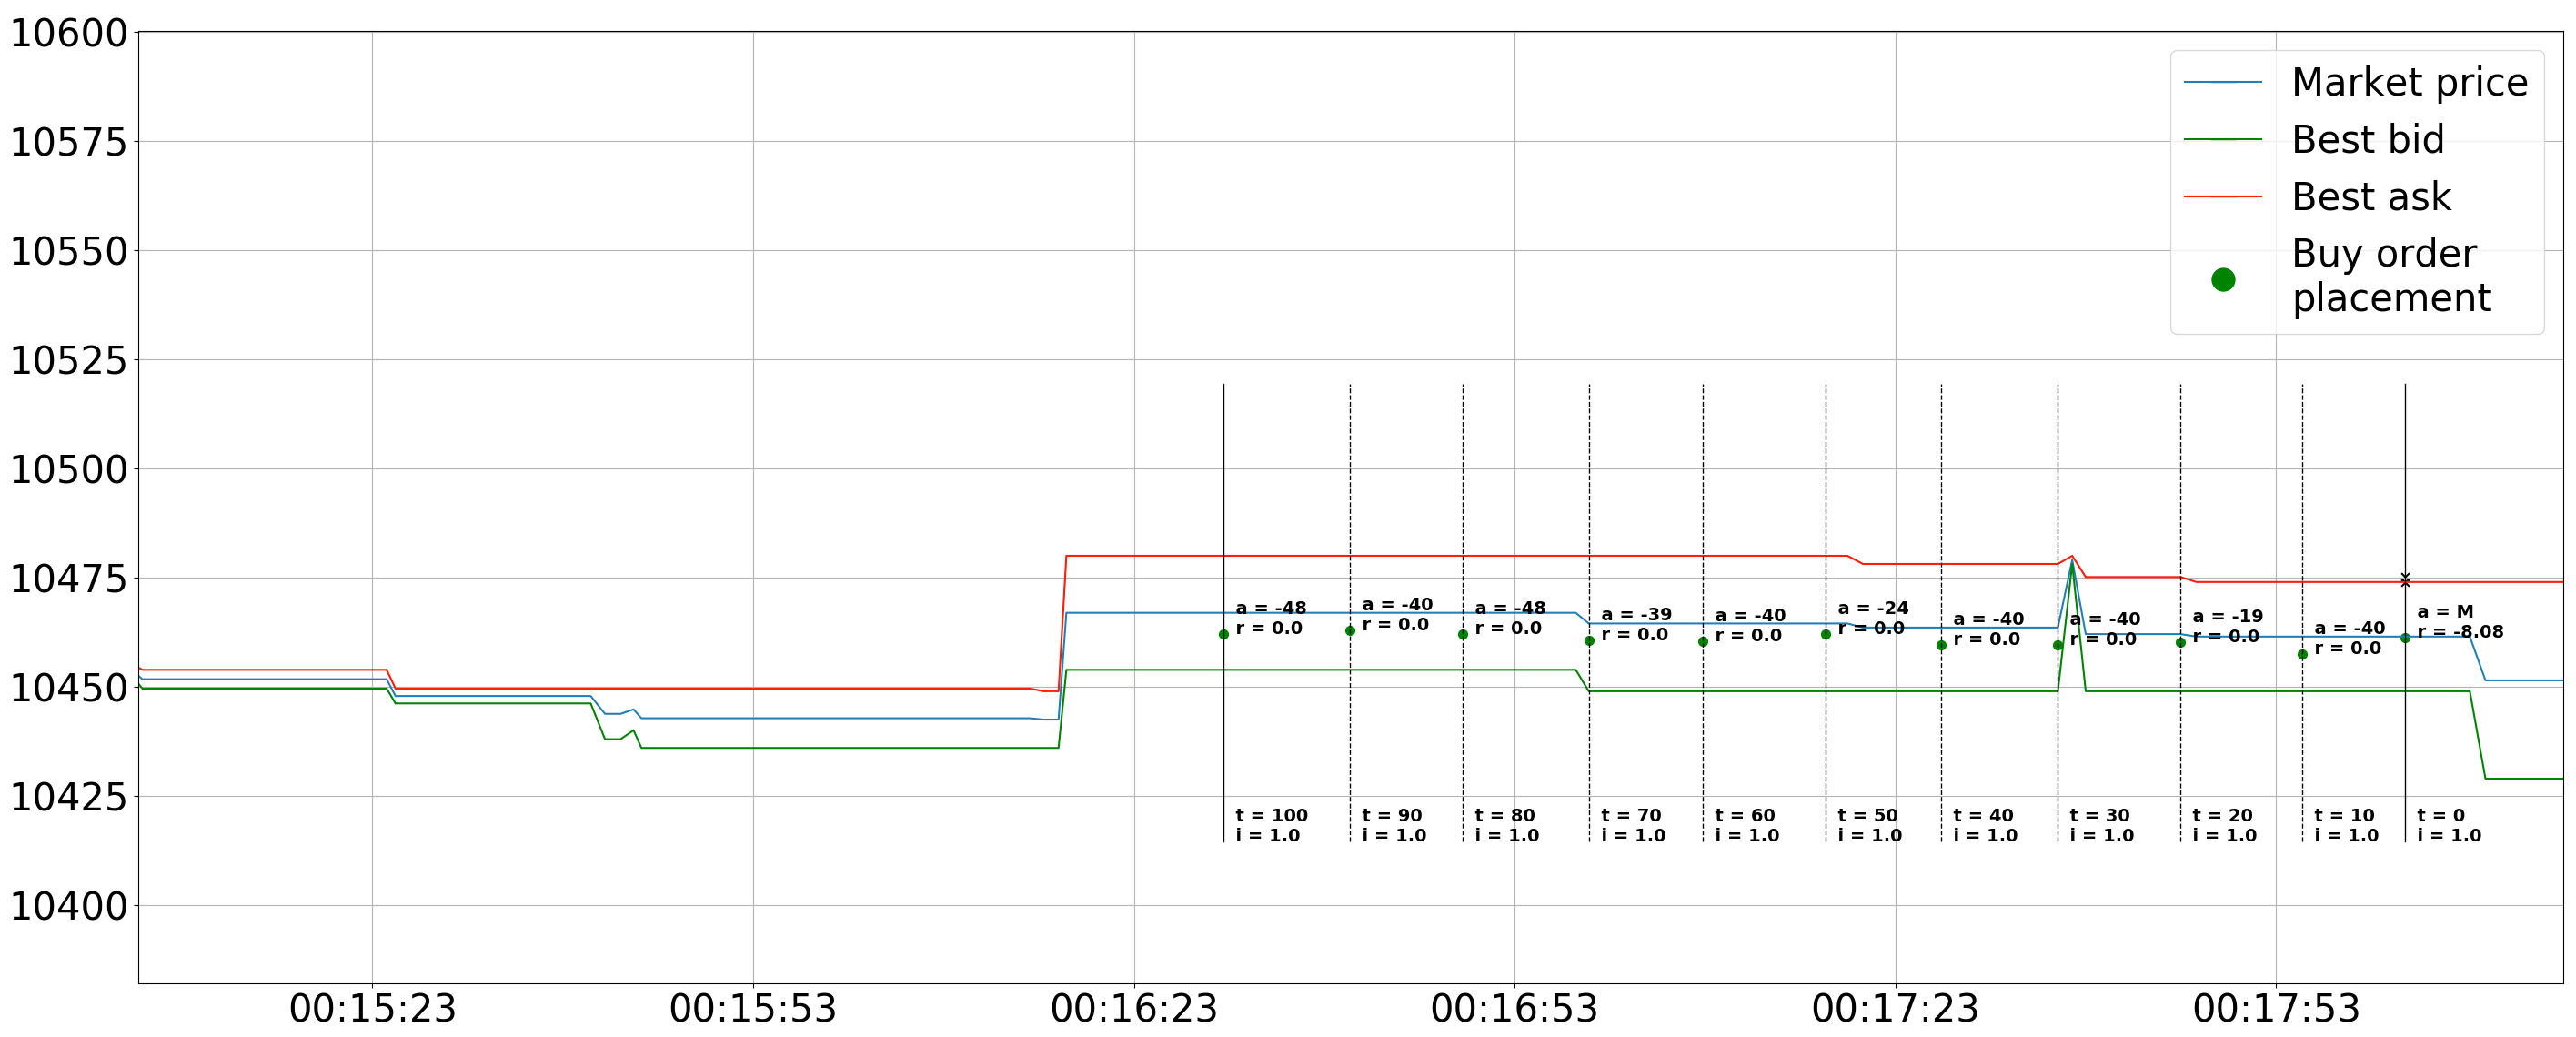
\includegraphics[width=\textwidth]{images/analysis-limit-wide-spread-buy}
    }
    \caption{Wide spread between bid and ask prevents agent from buying.}
    \label{fig:analysis-limit-wide-spread-buy}
\end{figure}
\begin{figure}[H]
    \centering
    \makebox[\linewidth]{
        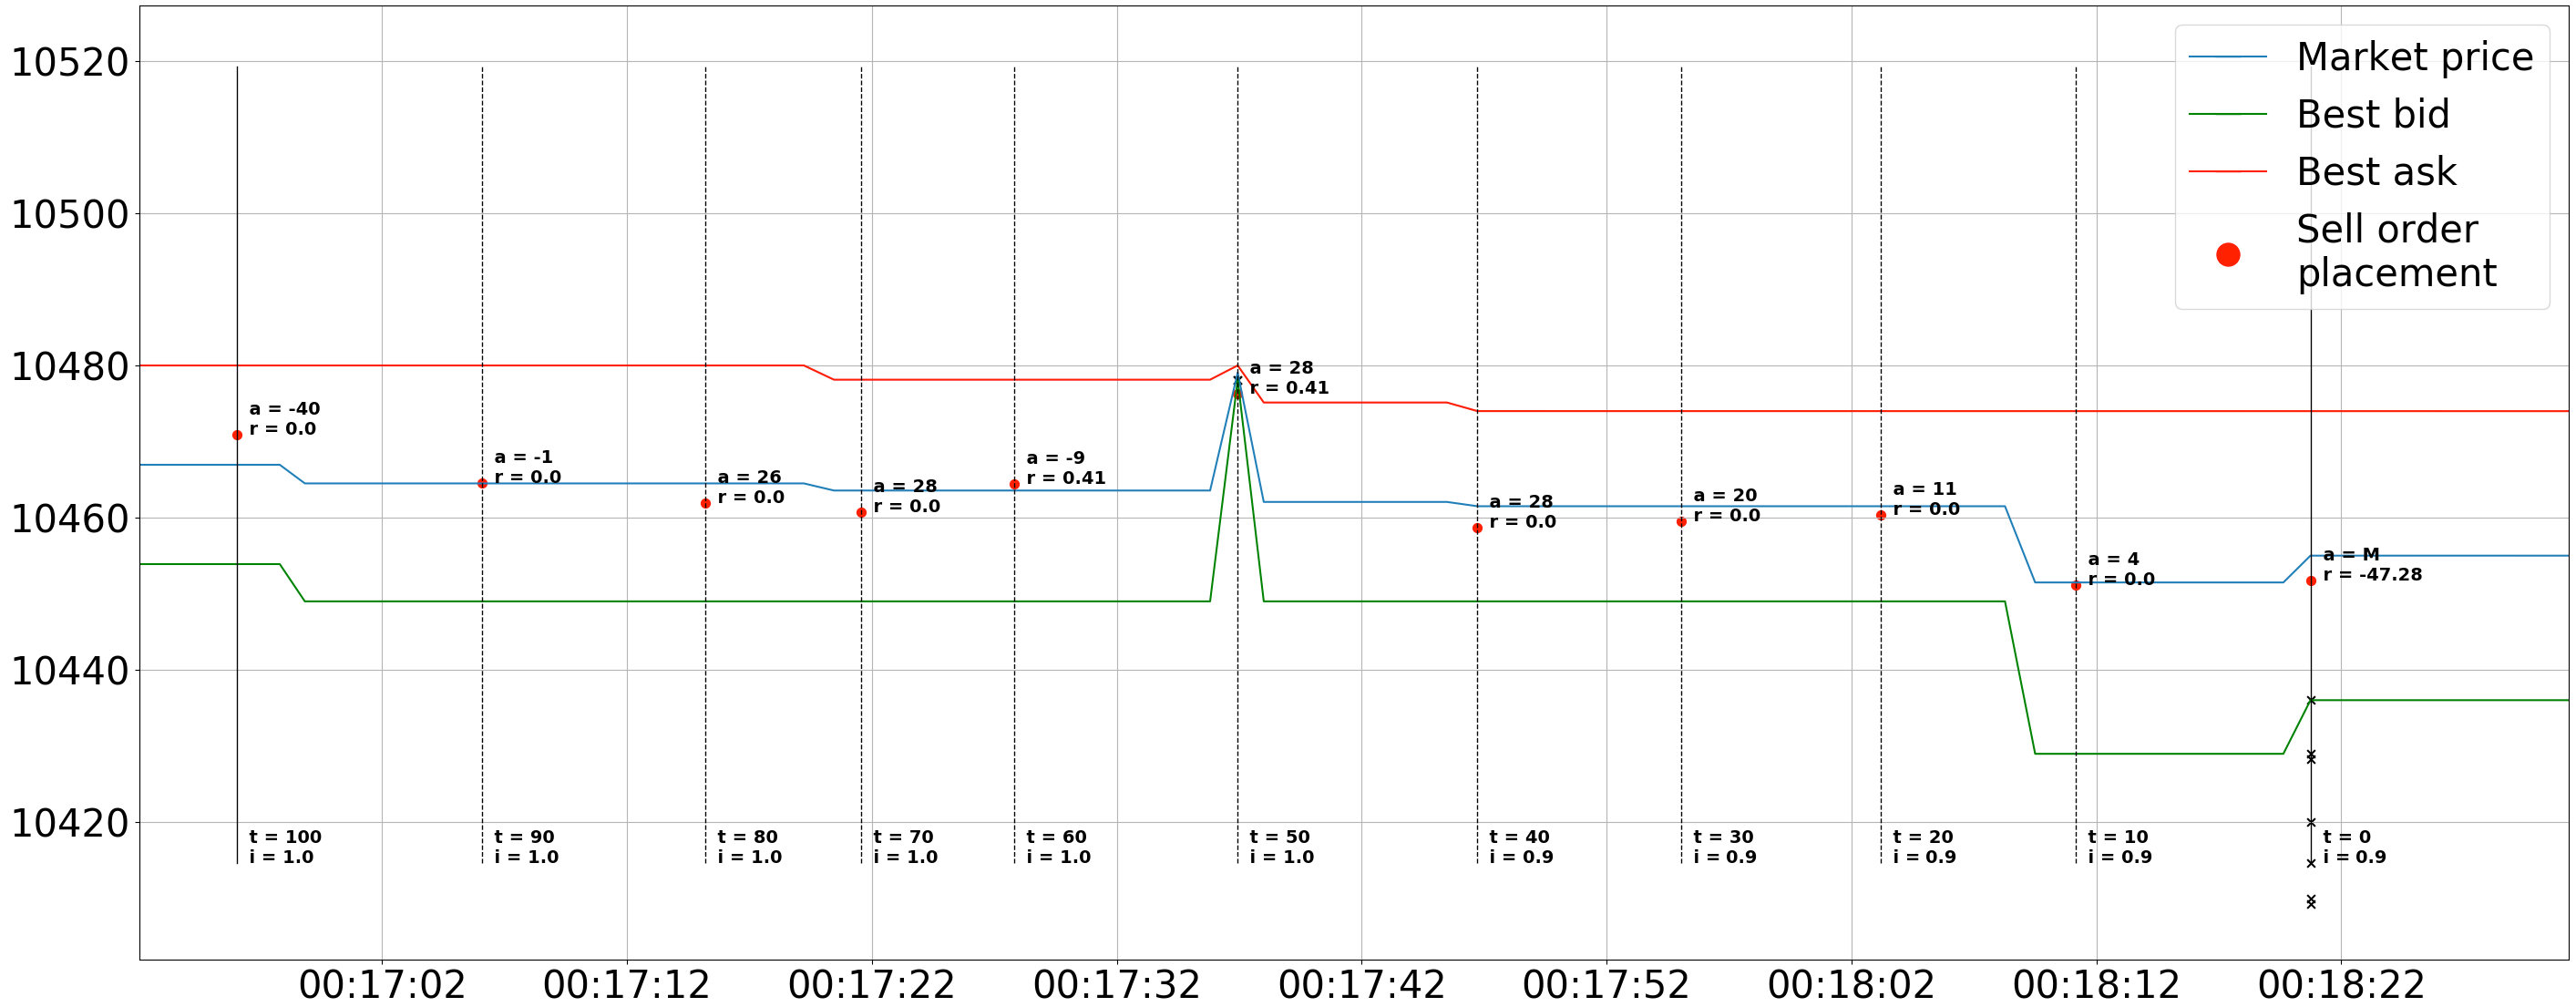
\includegraphics[width=\textwidth]{images/analysis-limit-wide-spread-sell}
    }
    \caption{Wide spread between bid and ask prevents agent from selling.}
    \label{fig:analysis-limit-wide-spread-sell}
\end{figure}
Prior to the start of the buy order placement, the spread was very close between the best bid and best ask price, as indicated by the green and red lines.
However, during the placement of this order, the spread widened and remained almost for the entire time horizon larger than \$50.00.
Since the actions are segmented in discrete steps of $\Delta{a}=0.10$, with a total of 101 steps, reaching from -\$5.00 to +\$5.00 relative to the market price, the agent had no chance of placing the orders close to the best ask price.
As a result, the entire inventory of 1.0 BTC bought by using a market order at the end of the time horizon (a trade is marked with a cross).
This generated a negative reward of -8.08.
The same market situation is demonstrated during which the agent initiated the process of placing a sell order.
Similarly, the pricing level was almost never close to the best bid price, except for once.
As a result, a market order was followed with which the agent sold the remaining 0.9 BTC to a decreased price that resulted in a negative reward of -47.28.
In addition, since there was not much liquidity offered by buyers, the market order was partially filled at decreasing price levels, as indicated by the crosses in the figure.
A way to overcome this limitation would be to either increase the number of steps or to increase the action step size and will be addressed in Chapter \ref{chap:discussion}.
\begin{figure}[H]
    \centering
    \makebox[\linewidth]{
        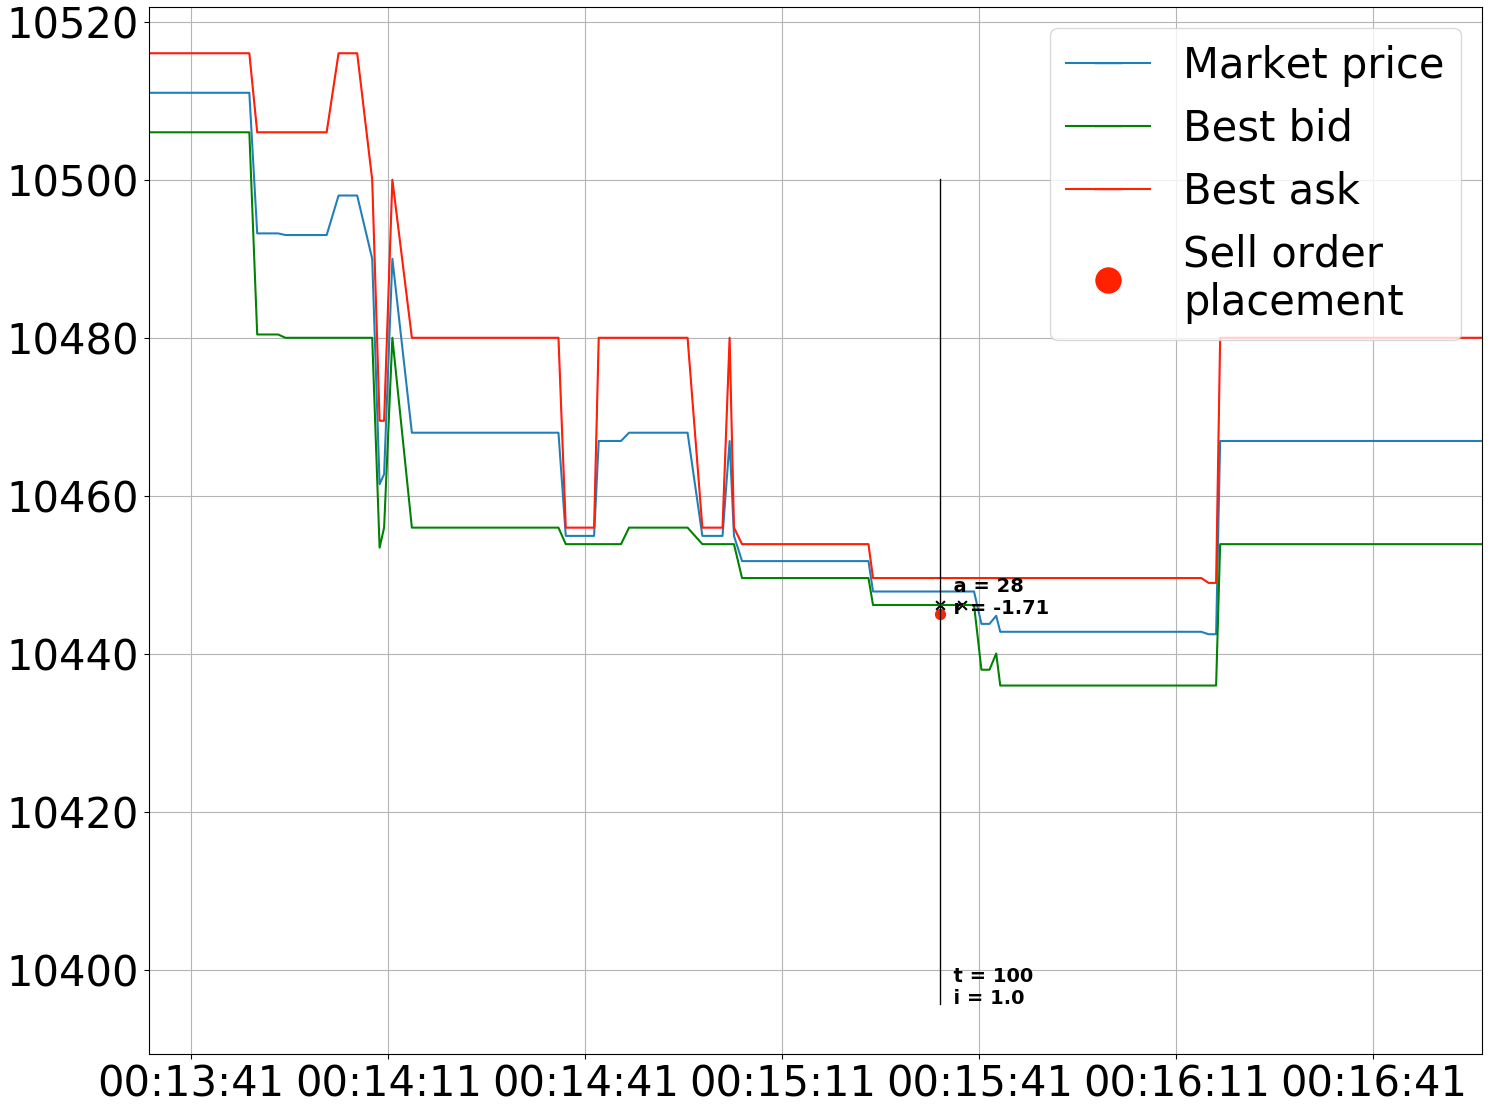
\includegraphics[width=10cm]{images/analysis-limit-impatient}
    }
    \caption{Wide spread between bid and ask prevents agent from selling.}
    \label{fig:analysis-limit-impatient}
\end{figure}
An example of the seconds category, where the agent clearly failed to select an appropriate action, is shown in Figure \ref{fig:analysis-limit-impatient}.
As is illustrated, the market price and the best bid and ask price were declining before the initialization of the sell order placement. 
The agent then decided to cross the spread with the first step and choose the action 28, in which it was willing to sell for \$2.80 below the market price.
By doing this, the order was immediately filled and resulted in a negative reward of -1.71.
Ideally, the agent should have been patient and decide to place a limit order below the spread.
Then, in a subsequent step, the order could have been filled with a negative action, which would have resulted in a positive reward.
It is to be assumed that the agent failed to generalize the development of the order book with the provided feature set.
Instead, the agent reacted according to the previous declining market situation, in which it would have been indeed the better choice to immediately fill the sell order.

\subsection{Capabilities evaluated using artificial limit order books}

Introducing an artificially created order book allows to determine the capabilities of a reinforcement learning agent in greater detail.
We define the formation of the order book states over time and therefore can calculate the optimal order placement policy in advance.
In doing this, we can investigate whether or not an agent is able to find the optimal placement policy.
In addition, by constructing such artificial order books, we are able to remove any short term market fluctuations and therefore provide more consistent rewards to the agent during training.
Figure \ref{fig:eval-limit-artificial} below shows the setup of two such order books.
Both consist of 10 minutes worth of data with order book states changing every 1 second, resulting in a total of 600 data points that represent the order book states.
Every such order book state consists of 25 levels on both the bid and ask side with a deviation of \$0.10 for each level, as shown in the zoomed panes.
In addition, on every such level 1.0 BTC is listed on the bid and ask side, which ensures that an agent can fill the entire order with any chosen limit level.
The change of the order book states is then determined by a function.
\begin{figure}[H]
    \centering
    \begin{subfigure}[b]{0.45\textwidth}
        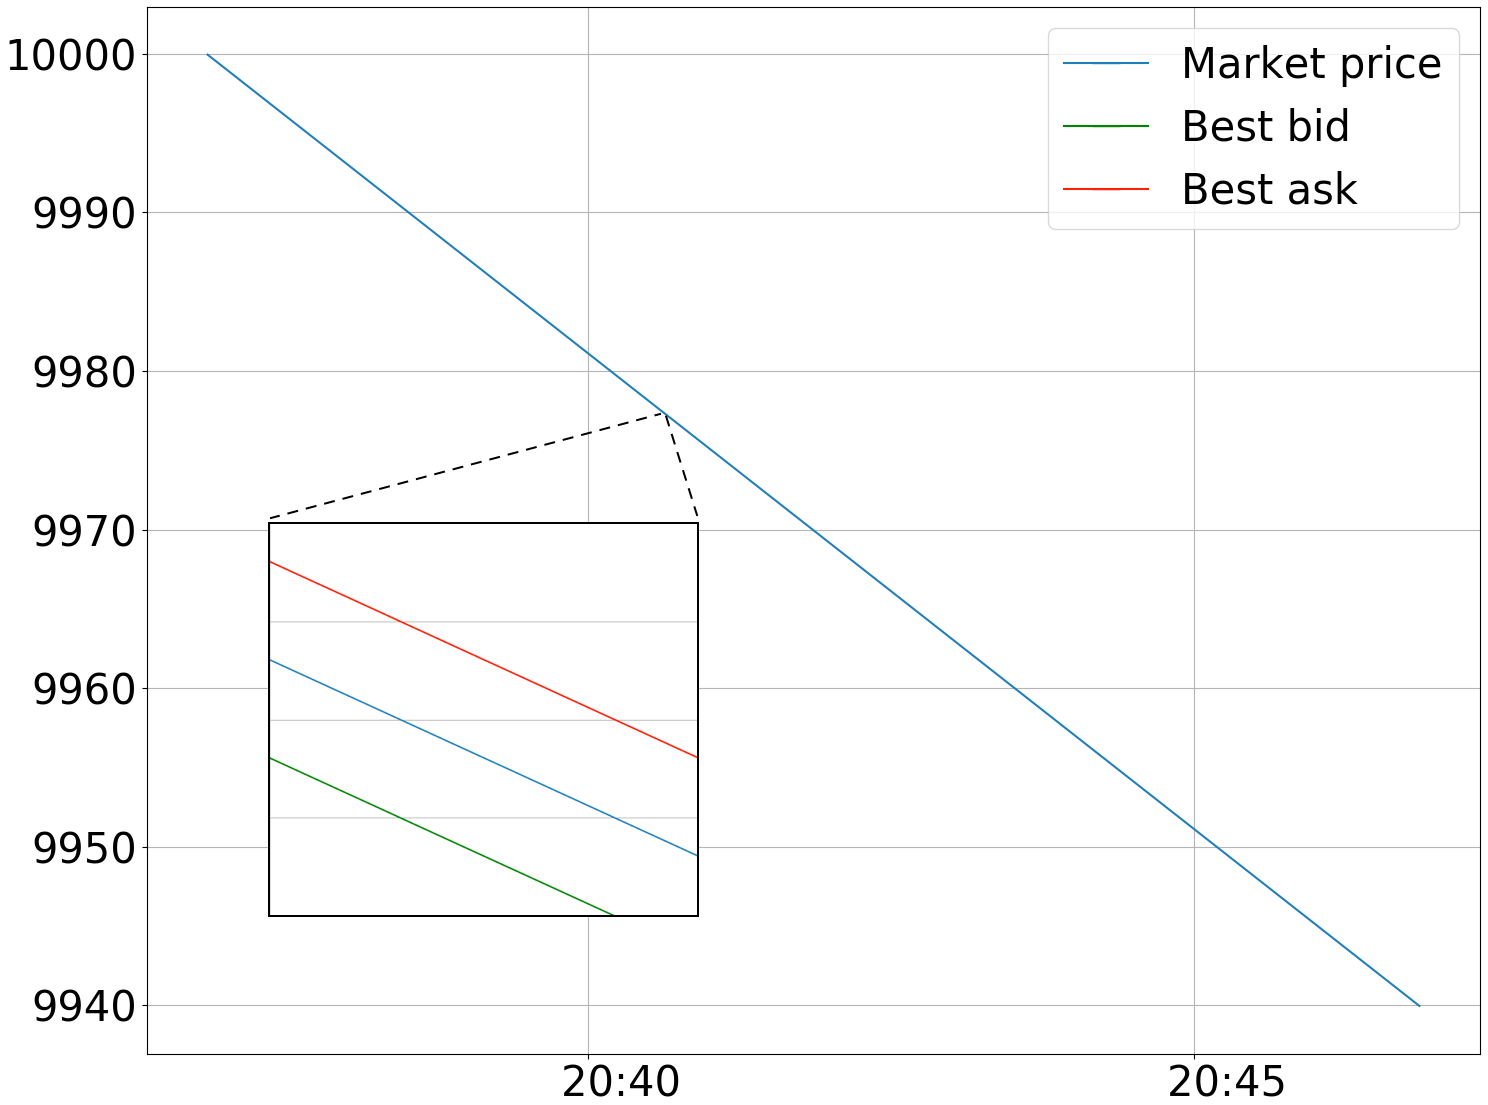
\includegraphics[width=\textwidth]{eval-limit-down}
        \caption{Linear configuration of order book states with slope $a=-0.1$}
        \label{fig:eval-limit-down}
    \end{subfigure}
    \begin{subfigure}[b]{0.45\textwidth}
        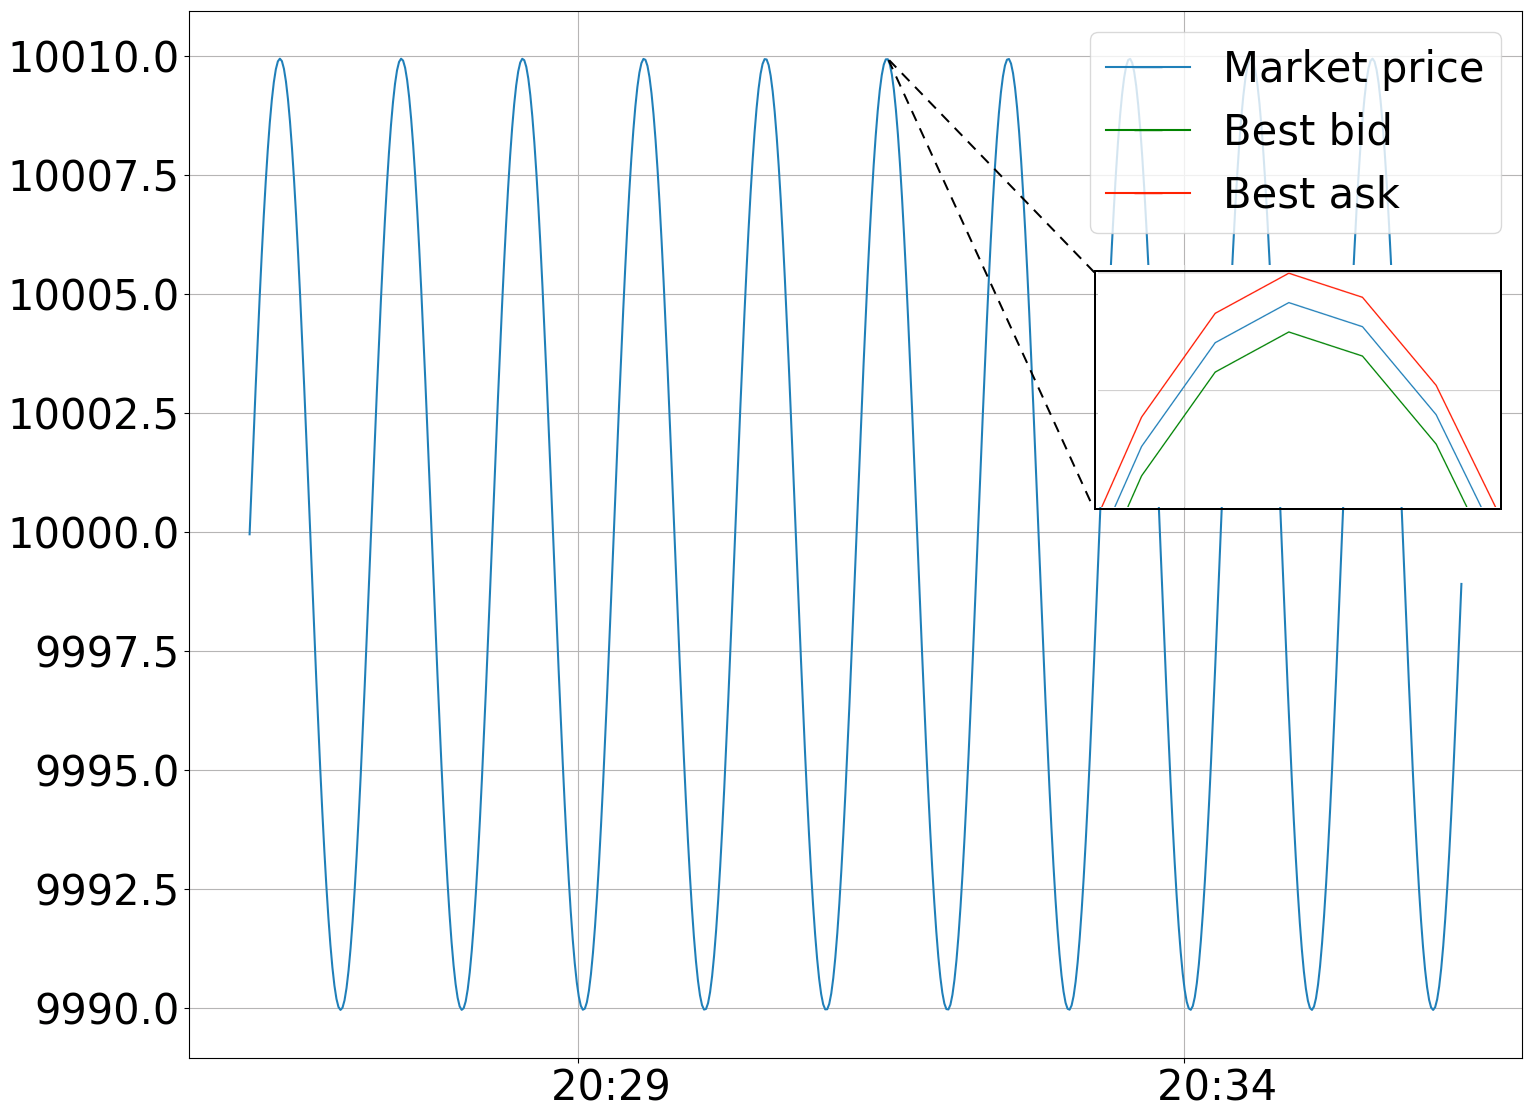
\includegraphics[width=\textwidth]{eval-limit-sine}
        \caption{Order book states configured according to sine function with $f=10$}
        \label{fig:eval-limit-sine}
    \end{subfigure}
    \caption{Artificial order books with duration of 10 minutes}\label{fig:eval-limit-artificial}
\end{figure}

The first example, as shown in Figure \ref{fig:eval-limit-down}, is a linear function which defines the market price to start at \$10'000 and end at \$9'940.
The price therefore falls by \$0.1 with every second.
An agent should therefore realize that for buying the actions chosen should be negative ($a<0$) for each step such that a trade transacts at the end of the time horizon to a much lower price.
The invariable reward after 100 seconds by choosing a random state to start the order placement, should therefore be \$10.0.
Contrarily, the agent should realize that the loss, when selling, can be minimized by selecting a very positive action that results in an immediate sale.
The invariable reward should therefore be -\$0.10.

The second example, as shown in Figure \ref{fig:eval-limit-sine}, applies a sine function over the order book states.
The frequency was set to 10 such that within one minute at least one complete sine wave is generated with the amplitudes peaking at \$10'010.0 and \$9'990.0 respectively.
An agent is expected to learn to place limit orders according to the low and high peak for buy and sell orders respectively.
The average reward for this example will not serve as an adequate measure since depending on which state the agent starts (e.g. at which point in the amplitude) the optimal rewards can be different.
Instead, we rely on the volume weighted average price directly and therefore expect the agent to buy close to \$9'990.0 and sell close to \$10'010.0.
\\
\\
Both artificial order book constellations, in form of feature type I, were trained and tested with the DQN agent.
The configuration of the agent was chosen equivalent to the setup described in Section \ref{sec:eval-dqn} and a total of 5000 epochs were proceeded for training and 1000 epochs for testing.
For the first example, that shows a clear downwards trend, the average reward during the backtest of buying assets resulted in \$9.45 and for selling in \$-0.10.
These results indicate that the agent was indeed able to find a near-optimal policy.
For the second example, that shows the multivariate sine wave that represents the order book, the average volume weighted average price for buying was \$9'992.0 and for selling \$10'007.0.
This indicates that the agent was able to improve to an near-optimal policy with regards to the fluctuating but stationary development of the order book.

\section{Conclusion of the evaluation}

With the evaluation procedure introduced and undergone in this chapter it was shown that reinforcement learning techniques are indeed suitable for optimizing limit order placement for cryptocurrency markets.
The findings are shown in Table \ref{tbl:analysis-conclusion}
First, we empirically estimated the potential improvements that can be achieved by placing orders with the the most optimal limit level compared to an immediate sale or purchase using a market order.
It has been shown that when the development of the market price comes in favor of the to limit order placement, namely when the price is falling while buying or when the price is rising while buying, then the reward for the optimal limit order is expected to be significantly higher.
In situations where the market price does not come in favor, then no improvement can be achieved and the optimal limit level is to cross the spread which declares the order to become a market order that fulfills the demand to buy or sell immediately.
Subsequently, the Q-Learning agent was trained and tested without the knowledge of market data but with private variables (inventory and time horizon) only.
The average rewards achieved during a backtest have shown that this agent was not able to take advantage of market price movements that come in favour of the order placement process.
However, the agent was able to reduce the costs when the market price development does not come in favor of either buying or selling assets.
In fact, the Q-Learning agent performed best among all considered agents, when it comes to reducing the occurrence of unavoidable losses.
Subsequently, the DQN agent was evaluated under the independent application of two feature sets.
It has been shown that the application of feature II (a sequence of historical trades) allows for a slightly better estimation of choosing actions for the limit order placement than the application of feature I (a window of historical order book states).
Although the DQN was able to learn a policy that allows to optimize the order placement when market conditions come in favor of buying or selling, the agent performed worse than the expected market order when conditions were not ideal.
In order to understand why no policy could be learned that would allow to constantly result in rewards better than the ones expected by using a market order, the actions taken by the DQN agent were analyzed.
It has been shown that 1) a wide spread between the best bid and ask price and 2) over-fitting on the given market features prevented the agent from choosing actions which would fill an order to a price better than the market price.
Furthermore, artificially created order books were created and features derived therefrom.
It was shown that in such a setting, where short term market fluctuations are absent and liquidity on the buyer and seller side is constantly provided, a deep reinforcement learning agent is able to find a near-optimal placement policy.
\begin{table}[H]
\centering
\caption{Summary of expected and achieved average rewards from empirical evaluations and reinforcement learning applications.}
\label{tbl:analysis-conclusion}
\begin{tabular}{l|l|l|l|l|l|}
\cline{2-6}
\textbf{}& \multicolumn{1}{c|}{\textbf{\begin{tabular}[c]{@{}c@{}}$\mathbb{E}$[Market \\ Order]\end{tabular}}} & \multicolumn{1}{c|}{\textbf{\begin{tabular}[c]{@{}c@{}}$\mathbb{E}$[Limit order]\\ (optimal)\end{tabular}}} & \multicolumn{1}{c|}{\textbf{Q-Learning}} & \multicolumn{1}{c|}{\textbf{\begin{tabular}[c]{@{}c@{}}DQN\\ (Feature I)\end{tabular}}} & \multicolumn{1}{c|}{\textbf{\begin{tabular}[c]{@{}c@{}}DQN\\ (Feature II)\end{tabular}}} \\ \hline
\multicolumn{1}{|l|}{\textbf{Buy (I)}}   & -0.05     & 15.20     & -1.17         & 22.06     & {\ul 31.92}   \\ \hline
\multicolumn{1}{|l|}{\textbf{Sell (I)}}  & -27.70    & -27.70    & {\ul -21.34}  & -39.26    & -25.15        \\ \hline
\multicolumn{1}{|l|}{\textbf{Buy (II)}}  & -1.06     & -1.06     & {\ul -1.04}   & -2.26     & -3.56         \\ \hline
\multicolumn{1}{|l|}{\textbf{Sell (II)}} & -1.72     & 3.38      & -4.74         & -0.84     & {\ul 0.15}    \\ \hline
\end{tabular}
\end{table}
